\documentclass[11pt]{article}
\usepackage[utf8]{inputenc}
 \usepackage[margin=2cm]{geometry}

\usepackage{amssymb,amsmath,amsthm,amsfonts}
\usepackage{amsmath,esint}
\usepackage{amsmath}
\usepackage{tocloft}
\usepackage{mathrsfs}
\usepackage{steinmetz}
\usepackage{cancel}
\usepackage{graphicx}
\usepackage{xcolor}

\usepackage{xparse}
\usepackage{amsmath}

\usepackage{tikz}
\usetikzlibrary{shapes.geometric, arrows}

\usepackage{graphicx}
\graphicspath{ {Bilder/} }

\usepackage{hyperref}
\hypersetup{
	colorlinks,
	citecolor=black,
	filecolor=black,
	linkcolor=black,
	urlcolor=black
}



% Frame setup
\usepackage{mdframed}
\mdfdefinestyle{minstil}{linecolor=black,linewidth=2pt}

\theoremstyle{definition}
\newtheorem{mindef}{Definisjon}[section]
\newenvironment{fmindef}
{\begin{mdframed}[style=minstil]\begin{mindef}}
		{\end{mindef}\end{mdframed}}



\theoremstyle{definition}
\newtheorem{mitteks}{Eksempel}[section]
\newenvironment{fmitteks}
{\begin{mdframed}[style=minstil]\begin{mitteks}}
		{\end{mitteks}\end{mdframed}}

\theoremstyle{definition}
\newtheorem{minset}{Setning}[section]
\newenvironment{fminset}
{\begin{mdframed}[style=minstil]\begin{minset}}
		{\end{minset}\end{mdframed}}

\theoremstyle{definition}
\newtheorem{teo}{Teorem}[section]
\newenvironment{fteo}
{\begin{mdframed}[style=minstil]\begin{teo}}
		{\end{teo}\end{mdframed}}


\theoremstyle{definition}
\newtheorem{regel}{Regel}
\newenvironment{fregel}
{\begin{mdframed}[style=minstil]\begin{regel}}
		{\end{regel}\end{mdframed}}

\theoremstyle{definition}
\newtheorem{formel}{Formel}
\newenvironment{fformel}
{\begin{mdframed}[style=minstil]\begin{formel}}
		{\end{formel}\end{mdframed}}

\renewcommand{\contentsname}{Innhold}


\NewDocumentCommand{\overarrow}{O{=} O{\uparrow} m}{%
	\overset{\makebox[0pt]{\begin{tabular}{@{}c@{}}#3\\[0pt]\ensuremath{#2}\end{tabular}}}{#1}
}
\NewDocumentCommand{\underarrow}{O{=} O{\downarrow} m}{%
	\underset{\makebox[0pt]{\begin{tabular}{@{}c@{}}\ensuremath{#2}\\[0pt]#3\end{tabular}}}{#1}
}

% Define block styles - Flytskjema

\tikzstyle{startstopp} = [rectangle, rounded corners, minimum width=3cm, minimum height=1cm,text centered, draw=black, fill=red!30]

\tikzstyle{prosess} = [rectangle , minimum height=1cm, draw=black, fill=cyan!30, text width=3cm, align=center ,rounded corners]

\tikzstyle{valg} = [diamond, minimum width=3cm,minimum height=1cm, text centered, draw=black, fill=cyan, aspect=2, text width=3cm ]

\tikzstyle{arrow} = [thick,->,>=stealth]


\newcommand{\MyTikzmark}[2]{%
	\tikz[overlay,remember picture,baseline] \node [anchor=base] (#1) {$#2$};%
}

\newcommand{\DrawVLine}[3][]{%
	\begin{tikzpicture}[overlay,remember picture]
	\draw[shorten <=0.3ex, #1] (#2.north) -- (#3.south);
	\end{tikzpicture}
}

\newcommand{\DrawHLine}[3][]{%
	\begin{tikzpicture}[overlay,remember picture]
	\draw[shorten <=0em, #1] (#2.west) -- (#3.east);
	\end{tikzpicture}
}

\author{Bjarte Mehus Sunde}

\begin{document}
	
    \title{MAT106 notater}
    \maketitle
    	
	\newpage
	
	\tableofcontents
	
	\newpage

	\section{Grunnleggende}
	
	\subsection{Potensregler}
	
	\begin{fregel}[Potensregler] \leavevmode
	\begin{enumerate}
		\item \(a^m\cdot a^n  = a^{(m+n)} \)
		\item \(\dfrac{a^m}{a^n}=a^{(m-n)} \)
		\item \(a^m + b^m = (a\cdot b)^m \)
		\item \(\dfrac{a^m}{b^m}=\left( \dfrac{a}{b}\right)^m  \)
		\item \((a^m)^n=a^{m\cdot n} \)
		\item \(a^{(-m)=\dfrac{1}{a^m}} \)
		\item \(a^0=1 \)
		\item \(a^{\frac{m}{n}}=\sqrt[n]{a^m}\)
	\end{enumerate}
	\end{fregel}
	
	
	\subsection{Kvadratsetningen}
	
	\begin{fteo}[\textbf{Kvadratsetningene}] \leavevmode
	\begin{enumerate}	
	    \item kvadratsetning: \( (a+b)^2 = a^2+2ab+b^2 \)
		\item kvadratsetning: \((a-b)^2=a^2-2ab+b^2 \)
		\item Kvadratsetning: \((a+b)(a-b)=a^2-b^2\)  \textit{(også kalt konjugatsetningen)}
	\end{enumerate}	
	\end{fteo}
	
	\newpage
	
	\subsection{ln}
	
	\begin{fregel} \leavevmode
		
	\begin{enumerate}
		\item \(ln\,ab=ln\,a+ln\,b\)
		\item \(ln\frac{a}{b}=ln\,a-ln\,b\)
		\item\(e^{ln\,a^k}=a^k\)
	\end{enumerate}
		
	\end{fregel}
	
	\newpage
	
	\subsection{Delbrøkoppspalting}
	  
	Fremgangsmåte
	\begin{enumerate}
		\item Ved \(\textit{polynomdivisjon}\) forenkler vi funksjonen til summen av et polynom og en rasjonal funksjon der telleren ar \textit{lavere grad} enn nevneren.
		\item Nevneren \textit{faktoriseres}.
		\item Ved \textit{delbrøkoppspalting} omskriver vi den rasjonale funksjonen videre til en sum av delbrøker av delbrøker av følgende to typer:
		\[\dfrac{A}{(x-a)^m}, \hspace{32pt} \dfrac{Bx+C}{(x^2+bx+c)^m} \]
	\end{enumerate}  
	  
	\begin{mitteks}
		Delbrøkoppspalt \(\dfrac{3x+11}{x^2-x-6} \)
		Det første vi må gjøre er å faktorisere nevneren så mye som mulig for å få det på en form vi kan bruke.
		\begin{align*}
		x^2-x-6&=0\\
		x^2-2\cdot \frac{1}{2}x+\left( \frac{1}{2}\right)^2&=6+\left( \frac{1}{2}\right)^2\\
		\left(x-\frac{1}{2}\right)^2&=\frac{25}{4}\\
		x&=\frac{1}{2}\pm \frac{5}{2}\\
		x=3 \hspace{16pt}&\text{eller}\hspace{16pt}x=-2\\
		(x-3)&(x+2) 
		\end{align*}
		Dette gir
		\[\dfrac{3x+11}{(x-3)(x+2)}=\dfrac{A}{x-3}+\dfrac{B}{x+2}\]
		der \(A\) og \(B\) er konstanter vi må bestemme. Vi multipliserer med faktorisert fellesnevner \((x-3)(x+2)\) på begge sider og forkorter:
		
		\begin{align*}
		\dfrac{3x+11}{(x-3)(x+2)}\cdot (x-3)(x+2) &=\dfrac{A}{x-3}\cdot (x-3)(x+2)+\dfrac{B}{x+2} \cdot (x-3)(x+2)\\
		3x+11&=A(x+2)+B(x-3)
		\end{align*}
		
		Det er to ulike måter å løse likningen på. En metode som alltid virker, men ofte er mer arbeid. Den andre metoden er raskere, men vil ikke alltide virke. Vi skal bruke den raske metoden i dette eksempelet.
		
		Det vi skal gjøre er å sette inn verdier for x for å finne A og B, vi bruker verdiene \(x=-2\) og \(x=3\) som vi fant tidligere.
		
		\begin{align*}
			&x=-2\hspace{32pt} 5=A\cdot0 + B\cdot(-5)\,\,\,\rightarrow \,\,\, B=-1\\
			&x=3\hspace{36pt}20=A\cdot5+B\cdot0\,\,\,\rightarrow\,\,\, A=4 
		\end{align*}
		
		\[\dfrac{3x+11}{x^2-x-6}=\dfrac{4}{x-3}-\dfrac{1}{x+2}\]
	\end{mitteks}
	 
	 Finner andre metoden her visst det skulle bli nødvendig å bruke den: http://tutorial.math.lamar.edu/Classes/CalcII/PartialFractions.aspx
	 \newpage
	 
	 \subsubsection{Heaviside cover-up method}
	 En metode for delbrøkoppspalting. Kan ikke brukes hvisnoen av uttrykkene er kvadrert.
	 
	 \begin{mitteks}
	 	\[\frac{s}{(s-1)(s-2)}=\frac{A}{s-1}+\frac{B}{s-2}\]

	 
	 Heaviside cover-up metoden: Se hva \(s\) i nevner på brøken med \(A\) i må være for at den skal bli \(0\). Hold så over hele høyre side og \(s-1\) på venstre side og sett inn for \(s\). Dette er svaret for \(A\). Gjenta for \(B\). Løsning:
	 
	 \(s\) for \(A\) må være 1
	 
	 \[\frac{s}{\cancel{(s-1)}(s-2)}=\cancel{\frac{A}{s-1}+\frac{B}{s-2}}\]
	 
	 \[s=1 \hspace{16pt} \rightarrow \hspace{16pt} A=\frac{1}{1-2}=-1 \]
	 
	 \(s\) for \(B\) må være 2
	 
	 \[\frac{s}{(s-1)\cancel{(s-2)}}=\cancel{\frac{A}{s-1}+\frac{B}{s-2}}\]
	 
	 \[s=2 \hspace{16pt} \rightarrow \hspace{16pt} B=\frac{2}{2-1}=2 \]
	 
	 Så
	 
	 \[\frac{s}{(s-1)(s-2)}=\frac{-1}{s-1}+\frac{2}{s-2}\]
	 
	 \end{mitteks}
	 
	 \begin{mitteks}
	 	
	 	\[\frac{1}{s(s-1)(s-2)}=\frac{A}{s}+\frac{B}{s-1}+\frac{C}{s-2}\]
	 	
	 	\begin{align*}
	 	s=0 \hspace{16pt}&\rightarrow \hspace{16pt} 
	 	A=\frac{1}{-1\cdot -2}=\frac{1}{2}
	 	\\
	 	s=1 \hspace{16pt}&\rightarrow \hspace{16pt}
	 	B=\frac{1}{1\cdot(1-2)}=-1
	 	\\
	 	s=2 \hspace{16pt}&\rightarrow \hspace{16pt}
	 	C=\frac{1}{2\cdot (2-1)}=\frac{1}{2}
	 	\\
	 	\end{align*}
	 	så
	 	\[\frac{1}{s(s-1)(s-2)}=\frac{A}{s}+\frac{B}{s-1}+\frac{C}{s-2}=\dfrac{\frac{1}{2}}{s}-\frac{1}{s-1}+\dfrac{\frac{1}{2}}{s-2}\]
	 \end{mitteks}
	 
	 \newpage
	 \subsection{LHopitals regel}
	 
	 \begin{fregel}
	 	Anta at funksjonene \(f(x)\) of \(g(x)\) er deriverbare, og at \(g^{\prime} (x)\neq 0 \) for alle \(x\) i et område rundt \(x=c\) men \(g^\prime (c)=0\) er tillat. Dersom grenseverdien
	 	\[\lim\limits_{x\rightarrow c}\frac{f(x)}{g(x)} \]
	 	er et \(\frac{0}{0}\) eller et \(\frac{\infty}{\infty}\) uttrykk, vil
	 	\[\lim\limits_{x\rightarrow c} \frac{f(x)}{g(x)}=\lim\limits_{x\rightarrow c} \frac{f^\prime (x)}{g^\prime (x)} \]
	 	
	 	så lenge den siste grenseverdien eksisterer eller er \(\infty \) eller \(-\infty \).
	 \end{fregel}
	 
	 \newpage
	 
	 \subsection{Regneregler for n-fakultet}
	 
	Notasjonen \(n!\)(n-fakultet) betyr produktet av \(1\cdot 2\cdot 3\cdots n \) av heltallene fra 1 til \(n\). 
	\[4!=1\cdot 2\cdot 3\cdot 4 = 24 \]
	\[5!=\underbrace{1\cdot 2\cdot 3\cdot 4}_{4!}\cdot5=5\cdot 4! \]
	\[5!=\underbrace{1\cdot 2\cdot 3}_{3!}\cdot 4 \cdot5=5\cdot 4 \cdot 3! \]
	
	Vi definerer \(0!\) til å være \(1\).
	
	\[0!=1 \]
	
	Utvidelse av paranteser:

	\[n!=n\cdot (n-1)\cdot (n-2)...3\cdot 2\cdot 1 \]
	
	\[(n+1)!=(n+1)\cdot n! \]
	
    \[(n+2)!=(n+2)\cdot (n+1) \cdot n\cdot (n-1)\cdot (n-2)! \]
	
	\begin{mitteks}
		Forenkl \(\dfrac{(n+3)!}{(n+2)!} \)
		
		\begin{align*}
		\dfrac{(n+3)!}{(n+2)!}=\dfrac{(n+3)\cdot \cancel{(n+2)!}}{\cancel{(n+2)!}}=n+3 
		\end{align*}
	\end{mitteks}
	
	\begin{mitteks}
		Forenkl \(\dfrac{7!}{6!}\) \[\dfrac{7!}{6!}=\dfrac{7\cdot \cancel{6!}}{\cancel{6!}}=7 \]
	\end{mitteks}
	
	\newpage
    
    \subsection{Vekst av funksjoner}
    
    \[\text{{ Fakultet}}>\text{Eksponentsial}>\text{Ploynom}>\text{Logaritme}\]
    
    f.eks.
    \[ x!>e^x>x^2>lnx\]
    
    \newpage
    
    \subsection{Binomialformelen}
    
    \begin{fformel}
    	\[(x+y)^n=\sum_{k=0}^{n}\left( \begin{array}{cc}
    	n\\k
    	\end{array} \right)x^{n-k}y^k \]
    \end{fformel}
    
    \begin{mitteks}
    	Ekspander \((n+1)^4 \)
    	
    	Begynner med å finne alle \(\left( \begin{array}{cc}
    		n\\k
    	\end{array} \right)\), der \(n=4\). Bruker nCr knappen på kalkulatoren:
    	
    	\[C(4,0)=1 \hspace{16pt}C(4,1)=4 \hspace{16pt} C(4,2)=6\hspace{16pt} C(4,3)=4\hspace{16pt}C(4,4)=1\]
    		
    	Så setter vi inn i formelen
    	
    	\begin{align*}
    	&\underbrace{1\cdot n^4\cdot 1^0}_{k=0}+\underbrace{4\cdot n^3\cdot1^1}_{k=1}+\underbrace{6\cdot n^2 \cdot 1^2}_{k=2} + \underbrace{4\cdot n^1 \cdot 1^3}_{k=3}+
    	\underbrace{1\cdot n^0\cdot 1^4}_{k=4}\\
    	&=n^4+4n^3+6n^2+4n+1
    	\end{align*}
    \end{mitteks}
    \newpage
		
	\subsection{Absoluttverdi}	
		Løs likningen \(|2x-3|-4=3\)
		
		\begin{align*}
		|2x-3|-4&=3		\\
		|2x-3|&=7		\\
		(2x-3)&=7		\\
		2x&=10			\\
		x&=5
		\end{align*}
		
		\begin{align*}
		|2x-3|-4&=3		\\
		|2x-3|&=7		\\
		-(2x-3)&=7		\\
		-2x+3&=7		\\
		-2x&=4			\\
		x&=-2				
		\end{align*}
		
		\[x=-2 \,\,\, eller \,\,\, x=5\]
    \newpage 
    \section{Komplekse tall}
	
	\subsection{Komplekse tall}
	
	\begin{fmindef}
		La z være et komplekst tall. Realdelen til z skrives Re(z), og imaginærdelen til z skrives Im(z). Hvis \(z=a+bi\), er altså \[Re(z) \hspace{8pt} og \hspace{8pt} Im(z)\]
	\end{fmindef}
	
	Vi må huske reglen \[i^2=-1\]
	
	\subsection{i}
	
	\begin{fregel}[Regneregler for i]
		\begin{align*}
		i^1&=i \\
		i^2&=-1 \\
		i^3&=-i \\
		i^4&=1
		\end{align*}
	\end{fregel}
	
	For å rekne \(i\) med høyere potens enn 4 må vi konvertere den til den nærmeste potensen som kan deles på 4. 
	
	\begin{fmitteks}
		\[i^{99}=i^{96+3}=i^{(4\times 24)+3}=i^3=-i\]
	\end{fmitteks}
	
	\newpage
	
	\subsection{Konjuglasjon}
	
	Når vi skal definere divisjon, trenger vi en operasjon som bytter fortegnet på imaginærdelen til et komplekst tall. Denne operasjonen dukker opp så ofte at den har fått et eget navn og en egen skrivemåte
	
	\begin{fmindef}
		Den \textit{konjugerte} til et komplekst tall \(z=a+bi\) er \[\bar{z}=x-yi\]
	\end{fmindef}
	
	\begin{fmitteks}
			La oss regne ut produktet av et komplekst tall z med det konjugerte tallet \(\bar{z}\).
			
			Setter vi inn \(z=x+yi\), får vi
			\begin{align*}
				z\bar{z}&=(x+yi)(\overline{x+iy}) \\
				&= (x+yi)(x-yi)                   \\
				&= x^2-(yi)^2                     \\
				&= x^2+y^2       
			\end{align*}
			Vi ser at z\(\bar{z}\) alltid blir et reelt tall! Dessuten er z\(\bar{z}\geq 0\) og z\(\bar{z} = 0\) hvis og bare hvis \(z=0\)
	\end{fmitteks}
	
	\newpage
	
	\subsection{Divisjon}
	
	\begin{fmindef}
		Hvis \(z=x+yi\) er et komplekst tall og \(c\neq 0\) er et reelt tall, definerer vi \[\dfrac{x+yi}{c}=\frac{x}{c}+\frac{y}{c}i\]
		Hvis \(z_1=x_1+y_1i\) og \(z_2=x_2+y_2i\), og \(z_2\neq 0\), så definerer vi
		 \[ \frac{z_1}{z_2}=\frac{z_1\overline{z_2}}{z_2\overline{z_2}} \]
		 siden dette blir et komplekst tall delt på et reelt tall forskjellig fra null.
	\end{fmindef}
	
	\begin{fminset}
		For alle komplekse tall z og w gjelder følgende: \\
        \begin{enumerate}
        	\item[a)] \(\overline{z+w}=\overline{z} + \overline{w}\)
        	
        	\item[b)] \(\overline{zw} = \overline{z} \cdot \overline{w} \)
        	
        	\item[c)] \( \overline{\overline{z}}=z  \)
        \end{enumerate}
	\end{fminset}
	
	\newpage
	
	\subsection{Andregradsligninger}
	Alle andregradslikninger kan løses 
	
	\begin{fmindef}
		En andregradsligning \[ax^2+bx+c=0\] der a, b og c er reelle tall, har som kjent løsningene \[x=\dfrac{-b\pm \sqrt{b^2-4ac}}{2a}\]
	\end{fmindef}
	
	
	\begin{fmitteks}
		Løs ligningen \[z^2-2z+5=0\] Andregradsformelen gir 
		\[z=\dfrac{-(-2)\pm \sqrt{(-2)^2-4\cdot 1 \cdot 5}}{2 \cdot 1}=\dfrac{2 \pm \sqrt{-16}}{2} \]
		Nå vet vi at de to kvadratrøttene til \(-16\) er \(\pm \sqrt{-16}=\pm 4 i \). Derfor blir \[z=\dfrac{2\pm 4i}{2}=1\pm 2i \]
	\end{fmitteks}
	
	
\newpage

	Har funnet en metode som er mykje lettare og raskere enn ABC-formelen:
	
	\begin{fmitteks}
		Løs ligningen \[z^2-8z+25=0\]
		Skriver likningen på formen \[a^2-2ab+b^2 = -25\]
		Vi bestemmer at \(a=z\) og \(2ab=8z\). Må finne \(b\) og sette in for \(b^2\), det eneste leddet som mangler.
		
		Vi har at \(2ab=8z\), setter inn \(a=z\) og får \(2zb=8z\). Dette gir videre \(b=\dfrac{8}{2}=4\). 
		\[2ab=8z=2\cdot \underbrace{z}_a \cdot \underbrace{4}_b\] 
		Det eneste du trenger å gjøre for å finne b er å dele tallet som ganges med \(z\) med \(2\). \(b^2\) blir da \[b^2=4^2\]
		Setter \(b^2\) inn på begge sider av ligningen og får
		\[z^2-2\cdot z\cdot 4+4^2=4^2-25\]
		Bruker 2. kvadratsetning, skriver om og rekner ut
		\begin{align*}
		(z-4)^2&=-9        \\
		z-4&=\pm \sqrt{-9} \\
		z-4&=\pm 3i        \\
		z&=4\pm 3i
		\end{align*}
	\end{fmitteks}
	
	Eksempel med rett føring
	
	\begin{fmitteks}
		\begin{align*}
		z^2+10z+30&=0 						 \\
		z^2+2\cdot 5\cdot z + 5^2 &= 5^2 -30 \\
		(z+5)^2&=-5                          \\
		z&=\underline{\underline{-5\pm i\sqrt{5}}}
		\end{align*}
	\end{fmitteks}
	
	\newpage
	
	\section{Geometrisk tolkning av komplekse tall}
	
	\begin{fmindef}
		Et komplekst tall \(z=yi\) med realdel \(0\) kaller vi et \textit{imaginært tall}
		
		Imaginærdelen til \(a+yi\) er det reelle tallet \(y\), og ikke det imaginære tallet \(yi\)
	\end{fmindef}
	
	\subsection{Vektoroperasjoner}
	
	\begin{fminset}
		l \(z\) og \(w\) være to komplekse tall og \(c\) et reelt tall. Betrakter vi \(z\) og \(w\) også som vektorer, gjelder følgende:
		\begin{enumerate}
			\item[a)] Summen av \(z+w\) som komplekse tall er lik vektorsummen \(z+w\) som vektor.
			\item[b)] Differansen \(z-w\) som to komplekse tall er lik vektordifferansen \(z-w\) som vektor.
			\item[c)] Produktet \(cz\) som tall er lik skalarproduktet \(cz\) som vektor.
		\end{enumerate}
	\end{fminset}
	
	\newpage
	
	\subsection{Polarkoordinater}
	
	\begin{fmindef}[Polarkoordinater]
		\[r^2=x^2+y^2 \hspace{16pt} x=r\, cos\theta \hspace{16pt} y=r\, sin\theta \hspace{16pt} tan\theta =\dfrac{y}{x} \]
	\end{fmindef}
	
	\begin{figure}[!ht]
		\centering
			\begin{tikzpicture}
			\begin{scope}[thick,font=\scriptsize]
			% Axes:
			% Are simply drawn using line with the `->` option to make them arrows:
			% The main labels of the axes can be places using `node`s:
			\draw [->] (-0.5,0) -- (8,0);
			\draw [->] (0,-0.5) -- (0,8);
			
			% Axes labels:
			% Are drawn using small lines and labeled with `node`s. The placement can be set using options
			\iftrue% Single
			% If you only want a single label per axis side:
			\draw (7,-3pt) -- (7,3pt);   \node [below] at (7,0) {$x$};
			\draw (-3pt,7) -- (3pt,7);   \node [left] at (0,7) {$y$};
			
			\else% Multiple
			% If you want labels at every unit step:
			\foreach \n in {-4,...,-1,1,2,...,4}{%
				\draw (\n,-3pt) -- (\n,3pt)   node [above] {$\n$};
				\draw (-3pt,\n) -- (3pt,\n)   node [right] {$\n i$};
			}
			\fi
			\end{scope}
			
			\draw[red, dashed, very thick] (0,7) -- (7,7) -- (7,0);
			\draw[cyan, very thick] (0,0) -- (7,7) node [black, left] at (3.5,3.5) {\(r\)};
			\draw[cyan, very thick] (7,7) circle [radius=0.1] node [black] at (7.3,7.3) {\(z\)};
			\draw [red,very thick,->] (2,0) arc (0:45:2cm);
			
			% Place the equation into the circle:
			\node [below right,gray] at (2,1.2) {\(\theta \)};
			\end{tikzpicture}
		\caption{Polarkoordinater \(r\) og \(\theta \)}
	\end{figure}
	
	Disse formlene  gjelder også når \(x\) eller \(y\) er negative. Vi kan nå skrive \(z=x+yi\) på følgende form \[z=r\, cos\theta + (r\, sin\theta )i = r(cos\theta + i\, sin\theta ) \]
	
	\newpage
	\begin{fmindef}
		Vi sier at \[z=x+yi\] er skrevet på kartesisk form, og at \[z=r(cos\theta + i\, sin\theta )  \]
		er skrevet på polarform eller trigonometrisk form. Istede for denne formen kan vi og skrive \[z=re^{\theta i}\]
		Denne skrivemåten kalles noen ganger eksponentiell form eller rett og slett polarform.
	\end{fmindef}
	
	\begin{fmindef}
		Hvis \(z\) er et komplekst tall, så skriver vi \(|z|\) for lengden til \(z\). Dersom \(z=a+bi\), er \[r=|z|=\sqrt{x^2+y^2} \]
	\end{fmindef}
	
	\subsection{Multiplikasjon}
	
	\begin{fteo}
		La \(z_1\) være et komplekst tall med lengde \(r_1\) og vinkel \(\theta_1 \). La \(z_2\) være et komplekst tall med lengde \(r_2\) og vinkel \(\theta_2 \). Da har produktet \(z_1z_2\) lengde \(r_1r_2\) og vinkel \(\theta_1 + \theta_2 \)
		
		\[z_1\cdot z_2=r_1 r_2e^{i(\theta_1 + \theta_2)} \]
	\end{fteo}
	
	\subsection{Divisjon}
	
	\begin{fteo}
				La \(z_1\) være et komplekst tall med lengde \(r_1\) og vinkel \(\theta_1 \). La \(z_2\) være et komplekst tall med lengde \(r_2\) og vinkel \(\theta_2 \). Da har kvotienten \(\dfrac{z_1}{z_2}\) lengde \(\dfrac{r_1}{r_2}\) og \(\theta_1 - \theta_2 \)
				
				\[\dfrac{z_1}{z_2}=\dfrac{r_1}{r_2}e^{i(\theta_1 -\theta_2)}\]
	\end{fteo}
	
	\newpage
	
	\subsection{Den komplekse eksponentialfunksjonen}

	\begin{fmindef}
			For et komplekst tall \(x+iy\) setter vi \[e^{x+iy}=e^x(cos\, y + i\, sin\, y) \]
	\end{fmindef}
	
	\begin{formel}[eulers formel]
\begin{equation}
	e^{i\theta}=cos\theta + i\, sin\theta 
\end{equation}
	\end{formel}
	
	\begin{fminset}
		For alle komplekse tall \(z_1\) og \(z_2\) gjelder \[e^{z_1+z_2}=e^{z_1}e^{z_2}\]
	\end{fminset}
	
	\subsection{Potenser av komplekse tall}
	
	\begin{fteo}
		La \(z=re^{\theta i}\) være et komplekst tall og \(n\) et helt tall. Da er \[z^n = r^n e^{n\theta i}\] Altså har n-te potens \(z^n\) lengde \(r^n\) og vinkel \(n\theta \).
	\end{fteo}
	
	\begin{formel}[Moivers formel]
		\begin{equation}
		(cos\theta + i\, sin\theta )^n =  cos(n\theta) + i\, sin(n\theta)
		\end{equation}		
	\end{formel}
	
	\newpage
	
	\subsubsection{Oppgaver med løsningsforslag}
		La \(z=x+yi\) der \(x=Re(z)\) og \(y=Im(z)\) . Husk også at \(|z|=\sqrt{x^2+y^2}\)
	
		Skissér løsningsmmengden i det komplekse planet.
	
	1)
	
	\[Im(z+i)=3\]
	
	Løsning:
	
	
	\begin{align*}
	Im(z+i)&=3		\\
	Im(x+yi+i)&=3   \\
	Im(x+i(y+1))&=3 \\
	y+1&=3          \\
	y&=2
	\end{align*}
	
	\begin{center}
		\begin{tikzpicture}
	\begin{scope}[thick,font=\scriptsize]
	% Axes:
	% Are simply drawn using line with the `->` option to make them arrows:
	% The main labels of the axes can be places using `node`s:
	\draw [->] (-5,0) -- (5,0) node [above left]  {$\Re\{z\}$};
	\draw [->] (0,-5) -- (0,5) node [below right] {$\Im\{z\}$};
	
	% Axes labels:
	% Are drawn using small lines and labeled with `node`s. The placement can be set using options
	\iffalse% Single
	% If you only want a single label per axis side:
	\draw (1,-3pt) -- (1,3pt)   node [above] {$1$};
	\draw (-1,-3pt) -- (-1,3pt) node [above] {$-1$};
	\draw (-3pt,1) -- (3pt,1)   node [right] {$i$};
	\draw (-3pt,-1) -- (3pt,-1) node [right] {$-i$};
	\else% Multiple
	% If you want labels at every unit step:
	\foreach \n in {-4,...,-1,1,2,...,4}{%
		\draw (\n,-3pt) -- (\n,3pt)   node [above] {$\n$};
		\draw (-3pt,\n) -- (3pt,\n)   node [right] {$\n i$};
	}
	\fi
	\end{scope}
	% The circle is drawn with `(x,y) circle (radius)`
	% You can draw the outer border and fill the inner area differently.
	% Here I use gray, semitransparent filling to not cover the axes below the circle
    \draw[thick, color=red] (-5,2) -- (5,2) ;
	% Place the equation into the circle:
	\node [above right,gray] at (1,2) {\(Im(z+i)=3\)};
	\end{tikzpicture}
	\end{center}
	
	\newpage
	
	2) \[|z-2|=1 \]
	
	Løsning:
	
	\begin{align*}
	|z-2|&=1			\\
	|x+iy-2|&=1			\\
	|x-2+iy|&=1			\\
	\sqrt{(x-2)^2+y^2}&=1\\
	(x-2)^2+y^2&=1^2
	\end{align*}
	
	Dette er en sirkel med origo i \((2,0)\) og radius \(1\) \vspace{16pt}
	
\begin{center}
	\begin{tikzpicture}
	\begin{scope}[thick,font=\scriptsize]
		% Axes:
		% Are simply drawn using line with the `->` option to make them arrows:
		% The main labels of the axes can be places using `node`s:
		\draw [->] (-5,0) -- (5,0) node [above left]  {$\Re\{z\}$};
		\draw [->] (0,-5) -- (0,5) node [below right] {$\Im\{z\}$};
		
		% Axes labels:
		% Are drawn using small lines and labeled with `node`s. The placement can be set using options
		\iffalse% Single
		% If you only want a single label per axis side:
		\draw (1,-3pt) -- (1,3pt)   node [above] {$1$};
		\draw (-1,-3pt) -- (-1,3pt) node [above] {$-1$};
		\draw (-3pt,1) -- (3pt,1)   node [right] {$i$};
		\draw (-3pt,-1) -- (3pt,-1) node [right] {$-i$};
		\else% Multiple
		% If you want labels at every unit step:
		\foreach \n in {-4,...,-1,1,2,...,4}{%
			\draw (\n,-3pt) -- (\n,3pt)   node [above] {$\n$};
			\draw (-3pt,\n) -- (3pt,\n)   node [right] {$\n i$};
		}
		\fi
	\end{scope}
	% The circle is drawn with `(x,y) circle (radius)`
	% You can draw the outer border and fill the inner area differently.
	% Here I use gray, semitransparent filling to not cover the axes below the circle
	\path [draw,thick,color=red] (2,-0) circle (1);
	% Place the equation into the circle:
	\node [below right,gray] at (+2,1.7) {\(|z-2|=1\)};
\end{tikzpicture}
\end{center}
	
	\newpage

3) 	
	\[Re(z)-Im(z)\ge -2\]
	
	\begin{align*}
	Re(z)-Im(z) &\ge -2     \\
	x-y&\ge - 2 			\\ 
	x&\ge y-2
	\end{align*}
	\vspace{16pt}
	
		\begin{center}
			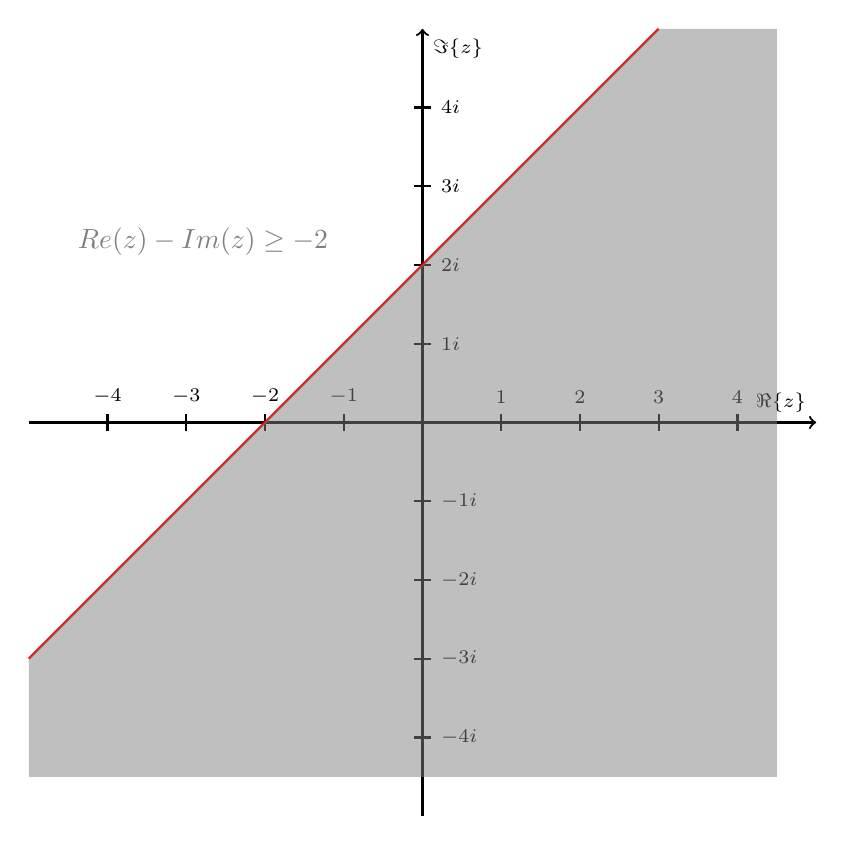
\begin{tikzpicture}
		\begin{scope}[thick,font=\scriptsize]
		% Axes:
		% Are simply drawn using line with the `->` option to make them arrows:
		% The main labels of the axes can be places using `node`s:
		\draw [->] (-5,0) -- (5,0) node [above left]  {$\Re\{z\}$};
		\draw [->] (0,-5) -- (0,5) node [below right] {$\Im\{z\}$};
		
		% Axes labels:
		% Are drawn using small lines and labeled with `node`s. The placement can be set using options
		\iffalse% Single
		% If you only want a single label per axis side:
		\draw (1,-3pt) -- (1,3pt)   node [above] {$1$};
		\draw (-1,-3pt) -- (-1,3pt) node [above] {$-1$};
		\draw (-3pt,1) -- (3pt,1)   node [right] {$i$};
		\draw (-3pt,-1) -- (3pt,-1) node [right] {$-i$};
		\else% Multiple
		% If you want labels at every unit step:
		\foreach \n in {-4,...,-1,1,2,...,4}{%
			\draw (\n,-3pt) -- (\n,3pt)   node [above] {$\n$};
			\draw (-3pt,\n) -- (3pt,\n)   node [right] {$\n i$};
		}
		\fi
		\end{scope}
		% The circle is drawn with `(x,y) circle (radius)`
		% You can draw the outer border and fill the inner area differently.
		% Here I use gray, semitransparent filling to not cover the axes below the circle
      	\draw[thick, color=red] (-5,-3) -- (3,5) ;
        \path [draw=none,fill=gray,semitransparent] (-5,-3) -- (3,5) -- (4.5,5) -- (4.5,-4.5) -- (-5,-4.5);
		% Place the equation into the circle:
		\node [above right,gray] at (-4.5,2) {\(Re(z)-Im(z)\ge -2\)};	
					 
		\end{tikzpicture}
		\end{center}
		
		\newpage
		
		\subsection{Røtter av komplekse tall}
		
		\begin{fmindef}
			Gitt et komplekst tall \(z\). Vi sier at et tall \(w\) er en \(n\)-te rot til \(z\) hvis \[w^n=z\]
		\end{fmindef}
		
\begin{fmindef}
			Metoden for å løyse slike oppgaver
		
		\begin{align*}
		w_0=\sqrt[n]{x+iy}&=\sqrt[n]{re^{i\theta}}=(re^{i\theta})^{\frac{1}{n}}=r^{\frac{1}{n}}e^{i\frac{\theta}{n}}\\
		w_1&=w_0e^{i\frac{2\pi}{n}} \\
		w_2&=w_1e^{i\frac{2\pi}{n}} 
		\end{align*}
\end{fmindef}
			
		\begin{mitteks}
			Finn \(\sqrt[3]{-8i} \):
			
			\[r=\sqrt{x^2+y^2}=\sqrt{0+(8)^2}=\sqrt{64}=8 \]
			
			Siden \(y=-8\) vet vi at vinkelen må vere
			
			\[\theta=\dfrac{3\pi }{2}\]
			
			\[w_0=\sqrt[3]{-8i}=(8e^{i\frac{3\pi}{2}})^\frac{1}{3}=8^{\frac{1}{3}}e^{i\frac{3\pi}{2}\frac{1}{3}}=2e^{i\frac{\pi}{2}}=2(cos(\tfrac{\pi}{2})+i\, sin(\tfrac{\pi}{2}))=\underline{2i}\]
			
			Kan ta en sjekk for å sjå at det stemmer
			
			\[(2i)^3=2i\cdot 2i\cdot 2i=4i^22i=-4\cdot2i=-8i\]
			
			\[\dfrac{2\pi}{n}=\frac{2\pi}{3}\Rightarrow e^{i\frac{2\pi}{3}}\]
			
			\[w_1=w_0e^{i\frac{2\pi}{3}}=2e^{i(\frac{\pi}{2}+\frac{2\pi}{3})}=2e^{i\frac{7\pi}{6}}=2\left( cos(\tfrac{7\pi}{6})+i\, sin(\tfrac{7\pi}{6})\right)=\underline{-\sqrt{3}-i},\,\,\, (-\sqrt{3}-i)^3=-8i \]
			\[w_2=w_1e^{i\frac{2\pi}{3}}=2e^{i(\frac{7\pi}{6}+\frac{2\pi}{3})}=2e^{i\frac{11\pi}{6}}=2\left( cos(\tfrac{11\pi}{6})+i\, sin(\tfrac{11\pi}{6})\right)=\underline{\sqrt{3}-i},\,\,\, (\sqrt{3}-i)^3=-8i \]


\[w_0=2i \hspace{16pt}w_1=-\sqrt{3}-i \hspace{16pt} w_2=\sqrt{3}-i \] 
		\end{mitteks}		
		\newpage
		
		\subsection{Komplekse andregradslikninger}
		
		\begin{fminset}
			For alle komplekse tall a, b og c med \(a\neq 0\) har ligningen \[az^2+bz+c=0\] alltid to komplekse løsninger, gitt ved formelen \[z=\dfrac{-b\pm \sqrt{b^2-4ac}}{2a}\] De to løsningene kan være like og kalles i så fall en dobbeltrot.
		\end{fminset}
		
		\begin{mitteks}
			Løs ligningen \[iz^2+(1-3i)z+2i-1\]
			Dette er en kompleks andregradsligning med koeffisienter \[a=i,\,\,\, b=1-3i, \,\,\, c=-1+2i \]
			
			Starter med å regne ut \(b^2-4ac\)
			\begin{align*}
			b^2-4ac&=(1-3i)^2-4i(-1+2i) \\
			&=1-6i+9i^2+4i-8i^2         \\
			&=-2i
			\end{align*}
			
			Finn løysningen på \(\pm\sqrt{-2i} \) ved å gjøre om til polarform
			\[r=2, \hspace{16pt} \theta=\frac{3}{2}\pi \]		
			\[\pm\sqrt{-2i} =\pm (2e^{i\frac{3}{2}\pi})^{\frac{1}{2}}=\pm \sqrt{2}(cos(\tfrac{3}{4}\pi)+i\, sin(\tfrac{3}{4}\pi))=\pm (-1+i)  \]
			Ligningen er nå \[z=\dfrac{-1+3i \pm (-1+i)}{2i}\]
			Det positive fortegnet gir
			\[z=\dfrac{-1+3i-1+i}{2i}=\dfrac{-1+2i}{i}\cdot \dfrac{-i}{-i}=2+i \]
			Det negative fortegnet gir
			 \[z=\dfrac{-1+3i+1-i}{2i}=\dfrac{2i}{2i}=1\]
			 Ligningen har de to løsningene 
			 \[z=2+i\hspace{16pt}og\hspace{16pt}
			 z=1. \]
		\end{mitteks}
		
		\newpage
		
		\subsubsection{Oppgaver med løsningsforslag}
		
		1) Løs ligningen: \[z^6-7z^3-8=0\]
		Setter \(z^3=u\)
		\[u^2-7u-8=0\]
		Skriver om ligningen så eg kan bruke 2. Kvadratsetning på den
		\begin{align*}
			u^2-2\cdot \dfrac{7}{2}\cdot u + \left( \dfrac{7}{2} \right)^2&=8+ \left( \dfrac{7}{2} \right)^2 \\
			\left(u-\dfrac{7}{2}\right)^2&=\dfrac{81}{4} \\
			u-\dfrac{7}{2}&=\pm \sqrt{\dfrac{81}{4}} \\
			u&=\dfrac{7}{2}\pm \dfrac{9}{2}
		\end{align*}
		\[u=8 \hspace{18pt} eller \hspace{18pt}u=-1\]
		
		Setter inn \(u=z^3\) og løyser først for \(u=8\)
		\[z^3=8, \hspace{18pt} r=8, \hspace{18pt} \theta=2\pi \]
		\begin{align*}
			z_0&=(8e^{i2\pi})^{\frac{1}{3}}=2e^{i\frac{2}{3}\pi}=2(cos\tfrac{2}{3}\pi+i\, sin\tfrac{2}{3}\pi)=-1+i\sqrt{3} \\
			z_1&=z_0e^{i\frac{2\pi}{3}}=2e^{i(\frac{2}{3}\pi+\frac{2}{3}\pi)}=2e^{\frac{4}{3}\pi}=-1-i\sqrt{3} \\
			z_2&=z_1e^{i\frac{2}{3}\pi}=2e^{i2\pi}=2
		\end{align*}
		
		Løyser så for \(u=-1\)
		
		\[z^3=-1, \hspace{18pt}r=1, \hspace{18pt} \theta=\pi \]
		\begin{align*}
			z_3&=\sqrt[3]{-1}=\left( e^{i\pi} \right)^{\frac{1}{3}}=e^{i\frac{\pi}{3}}=\frac{1}{2}+i\frac{\sqrt{3}}{2}\\
			z_4&=z_3e^{i\frac{2}{3}\pi}=e^{i\left( \frac{2}{3}\pi+\frac{1}{3}\pi \right)}=e^{i\pi}=-1\\
			z_5&=z_4e^{i\frac{2}{3}\pi}=e^{i\left( \frac{2}{3}\pi+\pi \right)}=e^{i\frac{5}{3}}=\frac{1}{2}-i\frac{\sqrt{3}}{2}
		\end{align*}
		\newpage
		
		\subsection{Faktorisering}
		
		\begin{fteo}[Alebraens fundamentalteorem]\leavevmode
			
			Ethvert polynom kan faktoriseres ved hjelp av komplekse
			
			 førstegradsfaktorer. Mer nøyaktig, anta at \[P(z)=a_nz^n+a_{n-1}z^{n-1}+...+a_1z+a_0 \]
			er et polynom av grad \(n\geq 1 \) med komplekse koeffisienter \(a_n\) og \(a_n\neq 0 \)
			
			Da finnes \(n\) komplekse tall \(z_1,z_2,...,z_n\) slik at
			\[P(z)=a_n(z-z_1)(z-z_2)(z-z_n)\]
			
		\end{fteo}
		
		\newpage
		
		\subsection{Visere}
		
		Alle komplekse tall kan skrives på formen
		\begin{equation}
			A\,e^{i\theta}=\underbrace{A\,cos\theta}_{Re(Ae^{i\theta})} + \underbrace{i\,A\,sin\theta}_{Im(Ae^{i\theta})}
			\hspace{38pt} \theta \,\,\,[Radianer] 
		\end{equation}
		
		Alle sinusformede bølgefunksjoner kan skrives på formen. 
		
		(Husk 		
		\(sin\theta=cos(\theta-\frac{\pi}{2}) \)) 
		\[v(t)=A\,cos(\overarrow[\omega][\downarrow]{{\tiny vinkelfrekvens}}t+\underarrow[\phi][\uparrow]{{\tiny fasevinkel}})\] 
		
		\[v(t)=Re\left( Ae^{i(\omega t+\phi)} \right)=Re\Big( \underbrace{Ae^{i\phi}}_{viser}e^{i\omega t} \Big)  \] 
		
		\begin{fmindef}
			Viser er den delen av spenningen på kompleks form som inneholder \(A\) og fasevinkel \(\phi \) 
			\[\textbf{V}=Ae^{i\phi}\]
			I elektrofag bruker man gjerne fasen i grader og innfører ny skrivemåte for dette 
			\[Ae^{i\phi}\text{ skrives da } A\phase{\phi^{\circ}} \]
		\end{fmindef}
		
		\begin{fmitteks}
			\[2\phase{45^{\circ}} \text{ er en viser} \]
			\[\text{Amplitude }2, \text{   Fasevinkel }45^{\circ}\]
		\end{fmitteks}
		
		\newpage
		
		Vil ofte summere mange sinusformede funksjoner \(y_i\) med samme frekvens \(\omega \) men ulik amlitude/fase
		
		\[y_i=a_ie^{i\phi_i}e^{ie^{i\omega t}}\]
		\[y_1+y_2+...+y_n=\underbrace{(A_1e^{i\phi_1}+A_2e^{i\phi_2}+A_ne^{e^{i\phi_n}})}_{\text{Sum av viserene}}e^{i\omega t} \]
		
		Trenger da å sumere
		\[ \textbf{Y}_1+\textbf{Y}_2+...+\textbf{Y}_n \,\,\, \text{for å finne dette}\]
		
		\begin{mitteks}
			Legg sammen funksjonene
			\begin{align*}
			y_1&=20cos\left( \omega t - \frac{\pi}{6}\right) \\
			y_2&=40cos\left(\omega t + \frac{\pi}{3}\right)
			\end{align*}
			
			Uten visere:
			
			\begin{align*}
			y_1+y_2&=20\left( cos \omega t \, cos \left(- \frac{\pi}{6}\right)+sin\omega t \,sin\left( \frac{\pi}{6} \right) \right)\\
			&+40\left( cos \omega t \, cos \left( \frac{\pi}{3}\right)-sin\omega t \,sin\left( \frac{\pi}{3} \right) \right)\\
			&=20\left( cos \omega t\cdot\frac{\sqrt{2}}{2}+sin\omega t \cdot \frac{1}{2} \right)\\
			&+40\left( cos \omega t\cdot\frac{1}{2}-sin\omega t \cdot \frac{\sqrt{3}}{2} \right)\\
			&=37.32cos\omega t - 24.64 sin \omega t = Acos(\omega t+\phi) = Acos\omega t \, cos \phi - Asin\omega t \, sin\phi 
			\end{align*}
			\begin{align*}
			&A\,cos\phi=37.32\\
			&A\,sin\phi=24.64\\
			(A\,cos\phi)^2+(A\,sin\phi)^2&=37.32^2+24.64^2=2000\\
			A^2(cos^2\phi+sin^2\phi)&=2000\\
			A^2&=2000\\
			A&=\underline{44.72} \\
			\frac{A\,sin\phi}{A\,cos\phi}=\frac{24.64}{37.32}&\rightarrow tan\phi=0.660 \rightarrow \phi=0.584\\
			y_1+y_2&=\underline{\underline{44.72cos(\omega t+ 0.584)}}
			\end{align*}
		\end{mitteks}
		
		\newpage
		
		Ved visere:
		
		\[\textbf{Y}_1=20\phase{-30^{\circ}}\hspace{32pt}\textbf{Y}_2=40\phase{60^{\circ}} \]
		
		\begin{align*}
		\textbf{Y}_1&=20\left( cos(-30^{\circ})+i\,sin(-30^{\circ}) \right)=10\sqrt{3}-10i\\
		\textbf{Y}_2&=40\left( cos(60^{\circ})+i\,sin(60^{\circ}) \right)=20+20\sqrt{3}i\\
		\textbf{Y}_1+\textbf{Y}_2&=(10\sqrt{3}+20)+(20\sqrt{3}-10)i=37.32+24.64i
		\end{align*}
		
		\[A=\sqrt{37.32^2+24.64^2}=44.72\]
		
		\[tan\phi=\frac{24.64}{37.32}=0.660 \rightarrow \phi=33.43^{\circ}\]
		
		\[\textbf{Y}_1+\textbf{Y}_2=44.72\phase{33.43^{\circ}}\]	


		\newpage
		\section{Følger}
		
		\begin{fmindef}
			En tallfølge er en oppstilling av tall i rekkefølge. 
			\[a_1,a_2,\, ...,a_n,\, ...\]
			Følgen består av relle tall \(a_n\), kalt leddene i følgen. 
		\end{fmindef}
		
		Hvis følgen har et endelig antall ledd er følgen endelig
		
		Hvis følgen har et uendelig antall ledd er følgen uendelig
		
		\begin{fmitteks}
			Følgen \[1,3,9,6,5,4,2,3\]
			er endelig, mens partallene 
			\[2,4,6,8,...,2n,...\]
			danner en uendelig følge.
		\end{fmitteks}
		
		Vi bruker notasjonen \(\left\lbrace a_n \right\rbrace^{\infty}_{n=1}\) for følgen \(a_1,a_2,...,a_n,...\) \vspace{8pt}
		
		Følgen av partall kan da skrives som \(\left\lbrace 2n \right\rbrace^{\infty}_{n=1} \)
		
		\newpage
		
	    \begin{mitteks}[Div. følger]
	    	\begin{list}{\(\bullet\)} \leavevmode
	    		\item Alle oddetallene \(\{2n-1\}^{\infty}_{n=1}\) er følgen \[1,3,5,7,...,2n-1,...\]
	    		\item Brøkene \(\left\lbrace \dfrac{1}{n} \right\rbrace^{\infty}_{n=1} \) er følgen 
	    		\[1,\frac{1}{2},\frac{1}{3},\frac{1}{4},...\]
	    		\item De samme brøkene, men med alternerende (vekslende) fortegn. 
	    		\(\left\lbrace (-1)^{n+1}\dfrac{1}{n} \right\rbrace^{\infty}_{n=1}\), er følgen 
	    		\[1,-\frac{1}{2},\frac{1}{3},-\frac{1}{4},...\]
	    		\item \(\left\lbrace \frac{1}{10^n}\right\rbrace^{\infty}_{n=1}  \) er følgen
	    		\[0.1,0.01,0.001,0.0001,...\]
	    		\item Husk at \(n!\) er produktet av tallene opp til \(n\), så \(\left\lbrace \dfrac{1}{n!} \right\rbrace^{\infty}_{n=1}\) er følgen \[1,\frac{1}{2},\frac{1}{6},\frac{1}{24},...\]
	    		\item \(\left\lbrace \dfrac{(-1)^n}{n(n+1)} \right\rbrace^{\infty}_{n=1}\) er følgen \[-\frac{1}{2},\frac{1}{6},-\frac{1}{12},\frac{1}{20},...\]
	    		\item \(\left\lbrace sin\dfrac{n\pi}{2} \right\rbrace ^{\infty}_{n=1}\) er følgen 
	    		\[1,0,-1,0,...\]
	    		\item \(\left\lbrace 1+(-1)^n \right\rbrace^{\infty}_{n=1}\) er følgen 
	    		\[0,2,0,2,...\]
	    		\item Primtallene er følgen \[2,3,5,7,11,13,...\]
	    		\item Desimalutvikling til \(\pi \), avkortet til \(n\) desimaler, er følgen \[3.1,3.14,3.141,3.1415,...\]
	    	\end{list}
	    \end{mitteks}
	    
	    \newpage
	    
	    \begin{fmitteks} [Følge gitt rekursivt] \leavevmode
	    	
	    	Fibonacci-følgen er gitt slik:
	    	\[F_1=1,\, F_2=1, \,\,\, og \,\,\, F_n=F_{n-1}+F_{n-2} \,\,\, for \,\,\, n\ge 3 \]
	    	Dette gir følgen
	    	\[1,1,2,3,5,8,13,21,34,55,...\]
	    \end{fmitteks}
	    
	    \begin{fmindef}[Begreper som beskriver følger] \leavevmode
	    	
	    	En følge \( \left\lbrace a_n\right\rbrace  ^{\infty}_{n=1}\) kalles
	    	\begin{list}{\(\bullet\)} \leavevmode
	    		\item oppad begrenset dersom det finnes et tall \(M\) slik at \(a_n\leq M \) for alle n 
	    		\item nedad begrenset dersom det finnes et tall \(M\) slik at \(a_n\ge -M\) for alle \(n\)
	    		\item begrenset dersom den er begrenset både nedad og oppad
	    		\item voksende dersom \(a_1\leq a_2 \leq a_3 \leq ... \leq a_{n+1} \leq ...\)
	    		\item strengt voksende dersom \(a_1 < a_2 < a_3 < ... < a_{n+1} < ...\)
	    		\item avtagende dersom \(a_1\geq a_2 \geq a_3 \geq ... \geq a_{n+1} \geq ...\)
	    		\item strengt avtagende dersom \(a_1 > a_2 > a_3 > ... > a_{n+1} > ...\)
	    		\item monoton dersom den er enten voksende elle avtagende
	    		\item positiv dersom \(a_n>0\) for all \(n\)
	    		\item alternerende dersom leddene \(a_1,a_3,...,a_{2n-1}, ...\) har motsatt fortegn av leddene \(a_2,a_4,...,a_{2n},...\)
	    	\end{list}
	    \end{fmindef}
	    
	    
		\newpage
		
		\subsection{Grenseverdi for følger}
		\begin{fmindef}
			\(\left\lbrace a_n \right\rbrace^{\infty}_{n+1} \) er en følge. Følgen konvergerer (mot \(L\)) dersom det finnes et tall \(L\) slik at vi kan få \(a_n\) så nær \(L\) vi ønsker ved å velge \(n\) tilstrekelig stor. Vi skriver da \[\lim\limits_{n\rightarrow \infty}a_n=L \]
			og vi sier at følgen konvergerer mot \(L\), og at \(L\) er følgen grenseverdi. Hvis følgen ikke konvergerer, sier vi at den divergerer.
		\end{fmindef}
		
		\begin{mitteks}
			\[	a_n=\dfrac{1}{n^2} \hspace{36pt}
			\lim\limits_{n\rightarrow \infty}\dfrac{1}{n^2}=0\]
			Følgen konvergerer mot 0.
		\end{mitteks}
		
		\begin{mitteks}
		  	\[	a_n=n^2 \hspace{36pt}
			\lim\limits_{n\rightarrow \infty}n^2=\infty\]	
	         Følgen divergerer mot uendelig.
		\end{mitteks}
		
		\begin{mitteks}
		 	\[	a_n=(-1)^n \hspace{36pt} a_n:1,-1,1,-1,1,-1,1,...\]			
		 	\(\lim\limits_{n\rightarrow \infty}a_n\) 
		 	eksisterer ikke. Følgen divergerer.
		\end{mitteks}

		\newpage

		\subsection{Divergens mot uendelig}
		 
		 \begin{fmindef}
		 	Vi ser at tallfølgen \(\left\lbrace a_n \right\rbrace^{\infty}_{n+1} \) divergerer mot uendelig dersom vi kan tvinge \(a_n\) til å bli så stor vi vil bare ved å kreve at \(n\) er tilstrekkelig stor, og skriver da
		 	\[\lim\limits_{n\rightarrow \infty}a_n=\infty \]
		 	Tilsvarende sier vi at følgen divergerer mot minus uendelig dersom vi kan tvinge \(a_n\) til å bli så negativ vi vil bare ved å kreve at \(n\) er tilstrekelig stor, og skriver da 
		 	\[\lim\limits_{n\rightarrow \infty}a_n=-\infty \]
		 \end{fmindef}
		 
		 \begin{mitteks}
		 	\[a_n=n! \hspace{36pt}\lim\limits_{n\rightarrow \infty}a_n=\infty \]
		 \end{mitteks}
		 
		 \begin{mitteks}
		 	\[a_n=1-e^n\hspace{36pt} \lim\limits_{n\rightarrow \infty}a_n=-\infty \]
		 \end{mitteks}
		 
		 \newpage
		 
		\subsection{Regneregler for følger}
		
		\begin{fteo}
			Hvis grensene \(\lim\limits_{n\rightarrow \infty}a_n=A\) og \(\lim\limits_{n\rightarrow \infty}b_n=B\)
			eksisterer, og \(c\) er en konstant, har vi:
			\begin{enumerate}
				\item \(\lim\limits_{n\rightarrow \infty}ca_n=cA\)
				\item \(\lim\limits_{n\rightarrow \infty}(a_n+b_n)=A+B\)
				\item \(\lim\limits_{n\rightarrow \infty}a_nb_n=AB\)
				\item \(\lim\limits_{n\rightarrow \infty}\dfrac{a_n}{b_n}=\dfrac{A}{B}\), forutsatt at \(B\neq 0\)
				\item \(\lim\limits_{n\rightarrow \infty}f(a_n)=f(A)\), forutsatt at funksjonen \(f(x)\) er kontinuerlig i \(x=A\) 
			\end{enumerate}  
		\end{fteo} 
		
		\begin{fteo}
			La \(f(x)\) være en funksjon med \(f(n)=a_n\) for alle naturlige tall \(n\). Hvis 
			
			\( \lim\limits_{n\rightarrow \infty } f(x) = L, \hspace{16pt} \)  så er   \(\hspace{16pt} \lim\limits_{n\rightarrow \infty}a_n=L \)
		\end{fteo}
		
		\begin{fteo}[Skviseteoremet for følger] \leavevmode
			
			Hvis \(a_n\leq b_n\leq c_n\) for alle \(n\). og 
			\[\lim\limits_{n\rightarrow \infty}a_n=L=\lim\limits_{n\rightarrow \infty}c_n \]
			er også \(\lim\limits_{n\rightarrow \infty}b_n=L\) 
		\end{fteo}
		
		\begin{mitteks}
			Vi skal vise at \[\lim\limits_{n\rightarrow\infty}\dfrac{(-1)^ncos\, n}{n^2}=0\]
			Dette følger greit av skviseteoremet fordi 
			\[-\dfrac{1}{n^2}\leq \dfrac{(-1)^ncos\, n}{n^2}\leq \dfrac{1}{n^2}\]
			og fordi \[\lim\limits_{n\rightarrow\infty}\dfrac{1}{n^2}=\lim\limits_{n\rightarrow\infty}\left( -\dfrac{1}{n^2}\right) =0\]
		\end{mitteks}
		
		\newpage
		
		\begin{fteo}[Konvergens av begrensede monotone følger]\leavevmode
			
			Enhver voksende følge som er oppad begrenset, konvergerer, og enhver avtagende følge som er nedead begrenset, konvergerer
		\end{fteo}
		
		\begin{mitteks}
\begin{flushleft}
				\[a_n=1+\dfrac{1}{n}\]
			Følgen er avtagende \(a_{n+1}<a_n\)		
				
			Følgen er nedad begrenset \(a_n>1\)
			
			\(\rightarrow\) Følgen konvergerer (mot 1)
\end{flushleft}
		\end{mitteks}
		
		\begin{mitteks}
			\[\lim\limits_{n\rightarrow \infty}\left(1+\dfrac{1}{n}\right)^{n}=e\]
			\[\lim\limits_{n\rightarrow \infty}\left(1-\dfrac{1}{n}\right)^{n}=
			\frac{1}{e}\]
			\[\lim\limits_{n\rightarrow \infty}\left(1+\dfrac{k}{n}\right)^{n}=e^k\]
		\end{mitteks}
		
		\newpage
		
		\section{Definisjon av rekke}
		
		\begin{fmindef}
			En rekke er en sum av uendelig mange ledd:
			\[\sum_{n=1}^{\infty }=a_1+a_2+...+a_n+... \]
		\end{fmindef}
		
		\begin{mitteks}
			\[\text{Tallfølge: } a_n=\dfrac{1}{2^n}\hspace{32pt} \dfrac{1}{2},\dfrac{2}{4},\dfrac{1}{8},\dfrac{1}{16},...\]
			\[\text{Rekke: }\sum_{n=1}^{\infty} \dfrac{1}{2^n} \hspace{32pt}\dfrac{1}{2}+\dfrac{1}{4}+\dfrac{1}{8}+\dfrac{1}{16}+... \]
		\end{mitteks}
		
		\subsection{Summen av en rekke}
		\begin{fmindef}
			Den \(N\)-te \textit{delsummen} av en rekke er summen av de \(N\) første leddene:
			\[S_n=a_1+a_2+...+a_N=\sum_{n=1}^{N}a_n\]
		\end{fmindef}
		
		\begin{fmindef}
			Dersom tallfølgen \(\left\lbrace S_n\right\rbrace \) er konvergent sier vi at rekken \(\sum_{n=1}^{\infty}\) er konvergent. 
			
			Hvis ikke sier vi at rekken divergerer.
		\end{fmindef}
		\newpage
		
		\subsection{Geometriske rekker}
		
		\begin{fmindef}
			Rekken \(\sum_{n=1}^{\infty}a_n\) kalles en \textit{geometrisk rekke} dersom hvert ledd etter det første er et fast multiplum av det foregående ledd, dvs. \(a_{n+1}=a_n\cdot r\). Tallet \(r\) kalles \textit{kvotienten}. Det generelle leddet kan skrives \(a_n=ar^{n-1}\), der \(a=a_1\) er det første leddet. Dette betyr at en geometrisk rekke er på formen 
			\[a+a\cdot r + a\cdot r^2 + a\cdot r^3 + ...=\sum_{n=1}^{\infty}a\cdot r^{n-1} \]		
		\end{fmindef}
		
		\begin{fmindef}
			Hvis \(|r|<1\) vil den geometriske rekken \(\sum_{n=1}^{\infty}a\cdot r^{n-1} \) konvergere. summen er 
			\[\sum_{n=1}^{\infty}a\cdot r^{n-1}=\dfrac{a}{1-r} \]
			Rekken divergere hvis \(|r|\geq 1\). For \(r\neq \)1 har vi følgende  uttrykk for delsummene:
			\[S_N=\sum_{n=1}^{N}a \cdot r^{n-1}=\dfrac{a(1-r^N
				)}{(1-r)} \]
		\end{fmindef}
		
		\begin{fregel}
			\[r=\dfrac{a_{n+1}}{a_n}\]
			\[a_n=r^{n-1}\]
			\[a \text{ er det første leddet!}\]
		\end{fregel}
		
		
		\begin{mitteks} 
			\[\sum_{n=1}^{\infty}\dfrac{1}{2^n}=\sum_{n=1}^{\infty}1 \cdot \left( \dfrac{1}{2} \right)^n=\sum_{n=1}^{\infty}\underbrace{1\cdot \frac{1}{2}}_{a_1}  \bigg( \overarrow[\dfrac{1}{2}][\downarrow]{r}  \bigg)^{n-1}= \dfrac{\frac{1}{2}}{1-\frac{1}{2}}=\underline{\underline{1} } \]
		\end{mitteks}
		
		\newpage
		
	    \subsubsection{Oppgaver med løsningsforslag}
	    	1)
	    	
	    	Avgjør om rekken konvergerer, hvis den gjør det, finn summen.
	    	\[16+8+4+2+1+...\]
	    \[a_1=16\]
	    \[r=\frac{a_n}{a_{n-1}}=\frac{a_2}{a_1}=\frac{8}{16}=\frac{1}{2}\]Sjekk og at r er lik for alle leddene. Sjekk så om rekken konvergerer:
	    \[|r|=\frac{1}{2}\hspace{32pt} |r|<1\rightarrow\text{ Den konvergerer!}\]
	    Finner så summen til rekken:
	    \[\sum_{n=1}^{\infty}a_1\cdot r^{n-1}=\dfrac{a_1}{1-r}=\dfrac{16}{1-\frac{1}{2}}=32\]
	    
	    2) 
	    
	    I en geometrisk rekke er det andre leddet lik 6 og det tredje leddet lik 4. Avgjør om rekken konvergerer, og finn i så fall summen.
	    
	    \[a_2=6 \,\,\, a_3=4 \]
	    
	    \[r=\frac{a_2}{a_1}=\frac{4}{6}=\frac{2}{3}\]
	    
		 \[a_{n-1}=\frac{a_n}{r}\rightarrow a_1=\frac{a_2}{r}=\frac{6}{\frac{2}{3}}=9 \]
		    
		 Sjekker om rekken konvergerer
		 
		 \[|r|=\frac{2}{3}\hspace{32pt} |r|<1\rightarrow\text{ Den konvergerer!}\]
		 
		 Finner så summen til rekken:
		 \[\sum_{n=1}^{\infty}a_1\cdot r^{n-1}=\dfrac{a_1}{1-r}=\dfrac{9}{1-\frac{2}{3}}=27\]
		 
	    \newpage
	    
	    3)
	    
	    I en geometrisk rekke er det tredje leddet lik 576 og det sjette leddet lik 243. Avgjør om rekken konvergerer, og finn i så fall summen.
	    
	    \[a_3=576 \hspace{32pt} a_6=243\]
		 
		Setter opp to ligninger med to ukjente:
	    
		\[a_1\cdot r^2=576  \,\,\text{ og }\,\, a_1\cdot r^5=243 \]		
		Løyser første for a
		\[a_1=\frac{576}{r^2}\]
		Setter den inn i den andre
	    \begin{align*}
	    a_1\cdot r^5 &= 243\\
	    \frac{576}{r^2}\cdot r^5&=243\\
	    r&=\sqrt[3]{\frac{243}{576}}=\frac{3}{4}
	    \end{align*}
	    
	    
	    Sjekker om rekken konvergerer
	    
	    \[|r|=\frac{3}{4}\hspace{32pt} |r|<1\rightarrow\text{ Den konvergerer!}\]
	    
		Finner a:
		\[a_2=\frac{a_3}{r}=\frac{576}{\frac{3}{4}}=768\]
		\[a_1=\frac{a_2}{r}=\frac{768}{\frac{3}{4}}=1024\]
		
		Finner til slutt summen av rekken:
		\[\sum_{n=1}^{\infty}a\cdot r^{n-1}=\dfrac{a}{1-r}=\dfrac{1024}{1-\frac{3}{4}}=4096\]
		\newpage
		
		4)
		
        I en konvergent geometrisk rekke med sum lik \(4\) er andre ledd lik \(-3\). Bestem det første leddet i denne rekken.
		
		\[1.\,\,\, \dfrac{a_1}{1-r}=4 \hspace{32pt} 2. \,\,\, r=\frac{a_2}{a_1}\hspace{32pt} a_2=-3\]
		
		Skal først finne r. Snur på ligningen 1
		\begin{align*}
		\dfrac{a_1}{1-r}&=4\\
		a_1&=4(1-r)
		\end{align*}
		
		setter inn i ligning 2
		
		\begin{align*}
		r&=\dfrac{a_2}{a_1} \\
		r&=\dfrac{-3}{4(1-r)} \\
		4r-r^2&=-3\\
		r^2-r&=\frac{3}{4}\\
		r^2-2\cdot \frac{1}{2}r+\left( \frac{1}{2} \right)^2&=\frac{3}{4}+\left( \frac{1}{2} \right)^2\\
		left(r-\frac{1}{2}right)^2&=1\\
		r&=\frac{1}{2} \pm 1  
 		\end{align*}
		\[r=-\frac{1}{2} \hspace{16pt} \text{eller} \hspace{16pt}r=\frac{3}{2}\]
		For at rekken skal konvergere må vi velge \(r=-\frac{1}{2}\), setter så inn i ligning 2 og løyser den:
		\begin{align*}
	    r&=\frac{a_2}{a_1}\\
	    a_1&=\frac{a_2}{r}\\
	    a_1&=\frac{-3}{-\frac{1}{2}}=\underline{\underline{6}}
		\end{align*}
		
		\newpage
		5)

		\[\sum_{n=0}^{\infty}(-1)^n\dfrac{5}{4^n} \]
				
		\[a=a_0=5 \hspace{16pt} a_1=-\dfrac{5}{4}\]
		\[r=\frac{a_1}{a_0}=\frac{-\frac{5}{4}}{5}=-\frac{1}{4}\]
		summen er \[\dfrac{5}{1-(-\frac{1}{4})}=4\]
		
		6)
		
		\[\sum_{n=0}^{\infty}e^{-2n}\]
		
		Bruker divergenstesten for å sjå om rekka konvergerer:
		\[\lim\limits_{n\rightarrow \infty}e^{-2n}=0 \rightarrow Konvergerer\]
		
		Skriver opp litt av rekka for å sjå etter mønster
		
		\[e^0+e^{-2}+e^{-4}+e^{-8}+...\]
		
		Ser at dette må være ei geometrisk rekke
		
		\[a=a_1=e^0=1\]
		\[r=\dfrac{e^{-4}}{e^{-2}}=e^{-4-(-2)}=e^{-2}=\dfrac{1}{e^2}\]
				
		Summen blir
		
		\[\dfrac{1}{1-\frac{1}{e^2}}=\dfrac{e^2}{e^2-1} \]		
		\newpage
		
		\subsection{Regneregler for rekker}
		\begin{fteo}[Ledvis addisjon og multiplikasjon]
			Hvis \(\sum_{n=1}^{\infty}a_n=A\) og \(\sum_{n=1}^{\infty}b_n=B\) og \(c\) er et reelt tall. Da er
			\begin{enumerate}
				\item \[\sum_{n=1}^{\infty}(a_n+b_n)=A+B\]
				\item \[\sum_{n=1}^{\infty}ca_n=cA \text{, der c er n konstant}\]
			\end{enumerate}
		\end{fteo}
		
		\begin{fteo}
			Hvis \(a_n\leq b_n\) for alle \(n\)
			\begin{enumerate}
				\item Hvis begge rekkene konvergerer, er \[\sum_{n=1}^{\infty}a_n=A\leq B=\sum_{n=1}^{\infty}b_n\]
				\item Om \(a_n > 0\) for alle \(n\), og \(\displaystyle{\sum_{n=1}^{\infty}b_n=B}\) konvergerer, er også \(\displaystyle{\sum_{n=1}^{\infty}a_n}\) konvergent
				\item Om \(a_n>0\) for alle \(n\), og \(\displaystyle{\sum_{n=1}^{\infty}a_n}\) divergerer mot uendelig, vil også \(\displaystyle{\sum_{n=1}^{\infty}b_n} \) divergere mot uendelig
			\end{enumerate}
		\end{fteo} 
		
		\newpage
		
		\subsection{Oppgaver med løsningsforslag}

		1)
		
		Finn summen til \(\displaystyle{\sum_{n=1}^{\infty}\dfrac{1}{n^2+5n+6}}\)
		
		Må bruke delbrøkoppspalting for å få eit uttrykk som er letter å jobbe med
		
		\begin{align*}
		n^2+5n+6=0\\
		(n+\frac{5}{2})^2=\frac{1}{4}\\
		n=-2 \hspace{16pt} n=-3
		\end{align*}
		\begin{align*}
		\dfrac{1}{(n+2)(n+3)}&=\frac{A}{n+2}+\frac{B}{n+3}\\
		1&=A(n+3)+B(n+2)\\
		n=-2 &\rightarrow A=1\\
		n=-3 &\rightarrow B=-1
		\end{align*}
		
		\[\sum_{n=1}^{k}\dfrac{1}{n^2+5n+6}=\sum_{n=1}^{k}\left(\frac{1}{n+2}-\dfrac{1}{n+3}\right)\]
		
		\begin{align*}
		S_k&=\left( \frac{1}{3}-\cancel{\frac{1}{4}} \right)+\left( \cancel{\frac{1}{4}}-\cancel{\frac{1}{5}} \right)+\left( \cancel{\frac{1}{5}}-\cancel{\frac{1}{6}} \right)+...+\left( \cancel{\frac{1}{k}}-\frac{1}{k+1} \right)\\
		S_k&= \frac{1}{3}-\frac{1}{k+1}
		\end{align*}
		Når \(k\rightarrow \infty\) vil \(S_k\rightarrow \frac{1}{3}\), så
		\[\displaystyle{\sum_{n=1}^{\infty}\dfrac{1}{n^2+5n+6}}=\underline{\underline{\frac{1}{3}}}\]
		
		
		
		\newpage
		
		\section{Konvergenstesting og summering av rekker}
		Ikke alle rekker \(\displaystyle{\sum_{n=1}^{\infty}a_n}\) er lette å summere. Det finnes allikevel måter å teste om en rekke er konvergent eller divergent uten å måtte beregne summen av rekken.
		\subsection{Divergenstesten}
		\begin{fteo}
			Hvis \(\displaystyle{\sum_{n=1}^{\infty}a_n}\) er en uendelig rekke og \[\lim\limits_{n \rightarrow \infty}a_n\neq 0, \] 
			divergerer rekken. Den divergerer også når grenseverdien ikke eksisterer
		\end{fteo}
		
		\begin{mitteks}
			\[\displaystyle{\sum_{n=1}^{\infty}2^n}\] divergerer, \(a_n=2^n\) \[\lim\limits_{n \rightarrow \infty
				}a_n=\infty \] 
				Grenseverdie eksisterer ikke
		\end{mitteks}
		
		\begin{mitteks}
			\[\displaystyle{\sum_{n=1}^{\infty}\dfrac{n}{n+1}}\] divergerer fordi \[\lim\limits_{n \rightarrow \infty}\left(\dfrac{n}{n+1}\right)=1\neq 0 \]
		\end{mitteks}
		
		\newpage
		
		\begin{mitteks}
			\[\sum_{n=1}^{\infty}\dfrac{1}{n}\] er grensen av leddene lik null ved utregningen
			\[\lim\limits_{n \rightarrow \infty}\dfrac{1}{n}=0 \]
			Divergenstesten gir ingen konklusjon. Derfor kan vi foreløpig ikke avgjøre om rekken konvergerer eller ikke. At leddene går mot 0 er en nødvendig betingelse for konvergens, men ikke tilstrekkelig. Vi skal snart se at denne rekken faktisk divergerer.
		\end{mitteks}
		
		\newpage
		
		\subsection{Leibniz-testen}
		Vi skal nå se på en test for rekker der leddene vekselvis er poisitve og negative. Disse rekkene er så vanlige at vi gir dem et navn:
		\begin{fmindef}
			En rekke kallesn \textit{alternerende} dersom to påfølgende ledd alltid har motsatt fortegn. Alternerende rekker kan skrives på formen \[\displaystyle{\sum_{n=1}^{\infty}(-1)^{n+1}a_n}\]
			med alle \(a_n>0\) eller alle \(a_n<0\)
		\end{fmindef}
		
		
		\begin{fteo}[Leibniz-testen] 
			Anta at \(\displaystyle{\sum_{n=1}^{\infty}(-1)^{n+1}}a_n\) er en alternerende rekke. Hvis
			\begin{list}{\(\bullet\)} \leavevmode
				\item Alle \(a_n\) er positive.
				\item størrelsen \(|a_n|\) på leddene er avtagende.
				 
				 \(|a_n|>|a_2|>...>|a_n|>|a_{n+1}|>...,\) \[a_{n+1}\leq a_n \]
				\item leddene går mot null, \(\lim\limits_{n \rightarrow \infty}a_n=0\),
			\end{list}
			er rekken konvergent. Hvis en rekke konvergerer ved denne testen, vil feilen \(E_N\) ved å avbryte summeringen etter \(N\) ledd oppfylle ulikheten \[|E_N|>|a_{N+1}|\]
		\end{fteo}
		
		\newpage
		
		\subsubsection{Oppgaver med løsningforslag}
		
		
		\begin{enumerate}
			\item Konvergerer rekken \(\sum_{n=1}^{\infty}(-1)^{n+1}\dfrac{1}{\sqrt{n}} \)
		 
		 \[a_n=\dfrac{1}{\sqrt{n}} > 0 \text{ for alle } n\geq 1 \]
		 
		 \[ n+1 \geq n \Rightarrow \sqrt{n+1} \geq \sqrt{n} \Rightarrow \frac{1}{\sqrt{n+1}} \leq\frac{1}{\sqrt{n}} \Rightarrow a_{n+1} \leq a_n \]
		 
		 \[\lim\limits_{n\rightarrow \infty}a_n = \lim\limits_{n\rightarrow \infty} \frac{1}{\sqrt{n}}=0\]
		 
		 Rekken konvergerer!
		
		
		\item Konvergerer rekken \(\sum_{n=2}^{\infty}(-1)^{n}\dfrac{4}{(ln\,n)^2}\)
		
		\[a_n = \dfrac{4}{(ln\,n)^2}>0 \text{ for alle } n\geq 2 \]
		
		\begin{align*}
		ln(n+1)\geq ln\,n &\Rightarrow (ln(n+1))^2 \geq (ln\,n)^2 \\ &\Rightarrow \dfrac{1}{(ln(n+1))^2} \leq \dfrac{1}{(ln\,n)^2} \Rightarrow \dfrac{4}{(ln(n+1))^2} \leq \dfrac{4}{(ln\,n)^2} \Rightarrow a_{n+1}\leq a_n 
		\end{align*}
		
		\[\lim\limits_{n\rightarrow \infty}a_n=\lim\limits_{n\rightarrow \infty}\dfrac{4}{(ln\,n)^2}=0 \]
		
		Rekken konvergerer!
		\end{enumerate}
		
		\newpage
		
		\subsection{P-rekke}
		
		\begin{fteo}
			Rekken \[\sum \dfrac{1}{n^p}\]
			konvergerer for \(p>1\) og divergerer for \(p\leq 1\)
		\end{fteo}
		
		\newpage

		 
		 \subsection{Integraltesten}
		 Det kan være vanskelig å overbevise seg om at rekker der leddene går mot null, likevel kan divergere. Dette eksempelet viser helt konkret at det skjer med rekken \(\displaystyle{\sum_{n=1}^{\infty}\frac{1}{n}}\). La oss se på følgen av delsummer. 
		 \[S_n=\sum_{n=1}^{N}\frac{1}{n}\]
		 I samme koordinatsystem som grafen til \(f(x)=\tfrac{1}{x}\), tegner vi bokser med høyden \(a_n=\tfrac{1}{n}\) og linjestykket \([n,n+1] \) som grunnflate. Vi ser at arealet av boksene er større enn arealet under grafen.
		 \[S_n>\int_{1}^{N+1}f(x)dx=[lnx]_{1}^{N+1}=ln(N+1) \]
        
         \begin{figure}[!ht]
	        \centering
		 	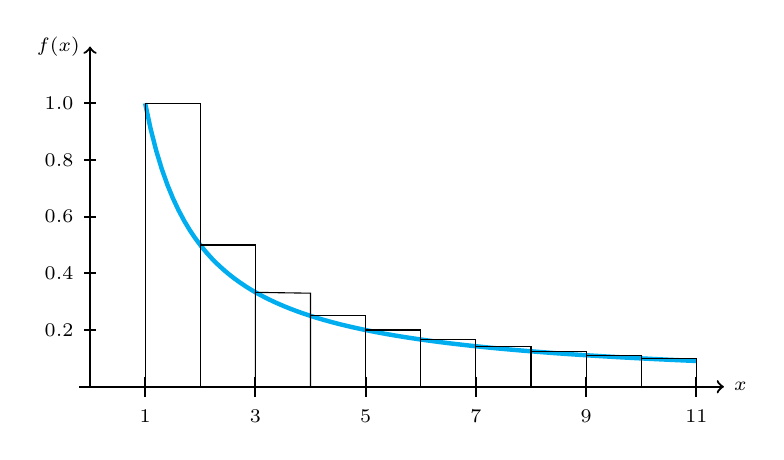
\begin{tikzpicture}[xscale=0.7,yscale=3.6]    				\begin{scope}[thick,font=\scriptsize]
		 	% Axes:
		    % Are simply drawn using line with the `->` option to make them arrows:
		 	% The main labels of the axes can be places using `node`s:
		 	\draw [->] (-0.2,0) -- (11.5,0) node [right] {\(x\)};
		 	\draw [->]  (0,0) -- (0,1.2) node [left] {\(f(x)\)};
		 	    				
			% Axes labels:
			% Are drawn using small lines and labeled with `node`s. The placement can be set using options
			\iffalse% Single
			% If you only want a single label per axis side:
		 	    				
		 	    				
		 	\else% Multiple
		 	% If you want labels at every unit step:
		 	\foreach \n in {1,3,...,11}{%
		 		\draw (\n,-1pt) -- (\n,1pt)   node at (\n,-3pt) {\(\n\)};
		 	}
		 	
		 	\foreach \n in {0.2,0.4,0.6,0.8,1.0}{%
		 		\draw (-3pt,\n) -- (3pt,\n) node at (-16pt,\n) {\(\n\)};
		 	}
		 
		 	
		 	\fi
		 	\end{scope}
		 	
            \draw[cyan, ultra thick, domain=1:11, samples=100] plot (\x, {1/\x});
		 	 	
	    	\draw (1,0) -- (1,1)     -- (2,1)      -- (2,0);
	        \draw (2,0) -- (2,0.5)   -- (3,0.5)    -- (3,0);
	        \draw (3,0) -- (3,0.333) -- (4,0.33)   -- (4,0);
	        \draw (4,0) -- (4,0.25)  -- (5,0.25)   -- (5,0);
	        \draw (5,0) -- (5,0.2)   -- (6,0.2)    -- (6,0);
	        \draw (6,0) -- (6,0.166) -- (7,0.166)  -- (7,0);
	        \draw (7,0) -- (7,0.142) -- (8,0.142)  -- (8,0);
	        \draw (8,0) -- (8,0.125) -- (9,0.125)  -- (9,0);
	        \draw (9,0) -- (9,0.111) -- (10,0.111) -- (10,0);
	        \draw (10,0) -- (10,0.1) -- (11,0.1)   -- (11,0);
			\end{tikzpicture}
			\caption{ \(1+\frac{1}{2}+...+\frac{1}{10}>\int_{1}^{11}\frac{1}{x}dx \)}
		 \end{figure}
		 	    		
		 Når vi lar \(N\rightarrow \infty\), ser vi at \[\sum_{n=1}^{\infty}\frac{1}{n}=\lim_{N \rightarrow \infty} \geq \lim_{N \rightarrow \infty} ln(N+1)=\infty\]
		 så rekken divergerer.		 
		 
		 \begin{fteo}
		 	La \(\displaystyle{\sum_{n=1}^{\infty}a_n}\) være en positiv rekke. Finn en funksjon \(f:[1,\infty)\rightarrow \Re \), med \(f(n)=a_n\). Anta at \(f(x)\) er avtagende i det minste for \(x\geq N \). Da konvergerer rekken \(\displaystyle{\sum_{n=1}^{\infty}a_n}\) hvis og bare hvis integralet \(\int_{N}^{\infty}dx\) konvergerer. Hvis rekken konvergerer ved denne testen, vil feilen vi gjør ved å avbryte summeringen etter \(N\) ledd, oppfylle følgende ulikhet:
		 	\[0\leq E_N \leq   \int\limits_{N}^{\infty}f(x)dx \]
		 \end{fteo}
		 
		 \begin{fmitteks}
		 	Divergerer elle konvergerer 
		 	\[\sum_{n=1}^{\infty}\frac{1}{n+4}\]
		 	Løser den med integraltesten
		 	\begin{align*}
		    \int_{1}^{\infty}\dfrac{1}{x+4}\,dx = 
		 	\lim\limits_{b\rightarrow \infty} \int_{1}^{b}\dfrac{1}{x+4}\,dx &=  \lim\limits_{b\rightarrow \infty} \left[ ln|x+4| \right]_{1}^{b}  \\
		    \lim\limits_{b\rightarrow \infty}(ln|b+4|-ln5)=\infty \rightarrow \int_{1}^{\infty}\dfrac{1}{x+4}\,dx \text{ divergerer } &\rightarrow \sum_{n=1}^{\infty}\frac{1}{n+4} \text{ divergerer } 	    
		 	\end{align*}
		 \end{fmitteks}
		 \newpage
		 
		 \subsection{Sammenligningstesten}
		 
		 \begin{fteo}
		 	La \(\sum a_n \) være en positiv rekke som skal testes for konvergens.
		 	\begin{enumerate}
		 		\item Dersom du finner en positiv konvergent rekke \(\sum b_n \) med \(a_n \leq b_n \) konvergerer også rekken \(\sum a_n \)
		 		\item Dersom vi finner en positiv divergent rekke \(\sum b_n \) med \(a_n \geq b_n \), divergerer også rekken \(\sum a_n \)
		 	\end{enumerate}		 \end{fteo}
		 	
		 	\begin{fminset}
		 		\begin{enumerate} \leavevmode
		 		\item Når du skal teste for \textbf{konvergens} skal du velge en \(b_n\) som er \textbf{større} enn \(a_n\)
		 		
		 		\item Når du skal teste for \textbf{divergens} skal du velge en \(b_n\) som er \textbf{lavere} enn \(a_n\)
		 		\end{enumerate}
		 	\end{fminset}
		 
		 \subsubsection{Oppgaver med løsningsforslag}
		 Bruk sammenligningstesten for å finne ut om rekka divergerer elle konvergerer
		 
		 1) \( \displaystyle{\sum_{n=1}^{\infty}} \dfrac{1}{n^2 +30} \)
		 
		 Sammenligner med \(\displaystyle{\sum_{n=1}^{\infty} \dfrac{1}{n^2} } \), som er en konvergent p-rekke, \(p=2>1\). 
		 
		 For \(n\geq 1 \) har vi:
		 
		 \[n^2 + 30 \geq n^2 \Rightarrow \dfrac{1}{n^2+30} \leq \dfrac{1}{n^2} \]
		 
		 Utifrå sammenligningstesetn konvergerer rekken
		 
		 2) \(\displaystyle{\sum_{n=2}^{\infty}} \dfrac{n+2}{n^2-n}\)
		 
		 Sammenligner med \(\displaystyle{\sum_{n=2}^{\infty}\dfrac{1}{n}} \), som er en divergent p-rekke, \(p=1\leq1\)
		 
		 \[n^2-n \leq n^2 \Rightarrow \dfrac{n}{n^2-1} \geq \dfrac{n}{n^2}=\dfrac{1}{n} \Rightarrow \dfrac{n+2}{n^2-n} \geq \dfrac{n}{n^2-1} \geq \frac{1}{n} \]
		 
		 Rekken diveregrer
		 
		 3) \(\displaystyle{\sum_{n=1}^{\infty}} \dfrac{cos^2n}{n^{\frac{3}{2}}} \)
		 
		  Sammenligner med \(\displaystyle{\sum_{n=1}^{\infty}\frac{1}{n^{\frac{3}{2}}}} \) som er en konvergent p-rekke, \(p=\frac{3}{2}>1\) 
		  
		  \[0\leq cos^2n \leq 1 \Rightarrow \dfrac{cos^2n}{n^{\frac{n}{3}}}\leq \dfrac{1}{n^{\frac{3}{2}}} \]
		  
		  Rekken konvergerer
		 \newpage
		 
		 \subsection{Grensesammenligningstesten}
		 
		 \begin{fteo}
		 	La \(\displaystyle{\sum_{n=1}^{\infty}a_n}\) og \(\displaystyle{\sum_{n=1}^{\infty}b_n}\) være positive rekker.
		 	\begin{enumerate}
		 		\item Anta at \(\displaystyle{\sum_{n=1}^{\infty}b_n}\) konvergerer og at \[0\leq \lim\limits_{n\rightarrow \infty}\dfrac{a_n}{b_n}<\infty,\] Da konvergerer også \(\displaystyle{\sum_{n=1}^{\infty}a_n}\)
		 		\item Anta at \(\displaystyle{\sum_{n=1}^{\infty}b_n}\) divergerer og at \[0<\lim\limits_{n\rightarrow \infty}\dfrac{a_n}{b_n}\leq \infty,\]Da diveregerer også \(\displaystyle{\sum_{n=1}^{\infty}a_n}\)
		 	\end{enumerate}
		 \end{fteo}
		 
		 For å finne \(b_n\) for p-rekker, brukes denne metoden:
		 
		 Finn \(b_n\) til \(\displaystyle{\sum_{n=1}^{\infty}\dfrac{n+1}{n^2\sqrt{n}}}\)
		 
		 For å finne \(b_n\) tar vi den dei leddene i teller og nevner med høgest potens for \(n\) og  forenkler. Vi ser her at \(\dfrac{n}{n^2\sqrt{n}} = \dfrac{n}{n^2\cdot n^{\frac{1}{2}}} = \dfrac{n}{n^{2+\frac{1}{2}}}=\dfrac{n}{ n^{\frac{5}{2}}}\)
		 
		 Vi tar no å trekker fra potensen til \(n\) i teller, både for \(n\) i teller og nevner. \(\dfrac{n^{1-1}}{n^{\frac{5}{2}-1}}=\dfrac{1}{n^{\frac{3}{2}}}\). Denne skal vi bruke som \(b_n\)
		 \[b_n=\dfrac{1}{n^{\frac{3}{2}}} \]
		 
		 
		 \newpage
		 
		 \subsection{Forholdstesten}
		 		
		 \begin{fmindef}[Forholdstesten]
		 	La \(\displaystyle{\sum_{n=1}^{\infty}a_n}\) være en rekke. Anta at grensen
		 	\[L=\lim_{n \rightarrow \infty}\left| \dfrac{a_{n+1}}{a_n} \right| \]
			eksisterer eller er \(\infty \). Da gjelder:
			\begin{enumerate}	 					\item Dersom \(L<1\), konvergerer    rekken.
		 	\item Dersom \(L>1\), divergerer rekken.
			\item Dersom \(L=1\), gir testen ingen konklusjon, prøv noe annet.
			\end{enumerate}
		 	Hvis rekken konvergerer ved punkt 1, og \(r\) er et tall slik at 
			\[1>r\geq \left| \dfrac{a_{n+1}}{a_n} \right|\hspace{16pt}\text{for alle }n\geq N, \]
		 	Vil feilen ved å avbryte summeringen etter \(N\) ledd oppfylle ulikheten
			\[|E_N|\leq \dfrac{|a_{N+1}|}{1-r} \]
		\end{fmindef}
		 
		 \begin{mitteks}
		 	\[\sum_{n=1}^{\infty}\dfrac{1}{n!}\hspace{36pt}a_n=\dfrac{1}{n!} \]
		 	\[L=\lim_{n \rightarrow \infty}\left| \dfrac{a_{n+1}}{a_n} \right|=\lim_{n \rightarrow \infty}\dfrac{\frac{1}{(n+1)!}}{\frac{1}{n!}}=\lim_{n \rightarrow \infty}\dfrac{n!}{(n+1)!}=\lim_{n \rightarrow \infty}\dfrac{1}{1+n}=0\]	
			Rekken konvergerer!
		 \end{mitteks}
		 		
		 \begin{mitteks}
			\[\sum_{n=1}^{\infty}\dfrac{(-1)^{n+1}}{n}\hspace{32pt}a_n=\dfrac{(-1)^{n+1}}{n} \]
			\[L=\lim_{n \rightarrow \infty}\left| \dfrac{a_{n+1}}{a_n} \right|= \lim_{n \rightarrow \infty}\left| \dfrac{\frac{(-1)^{n+1}}{n+1}}{\frac{(-1)^n}{n}}\right|=\lim_{n \rightarrow \infty}\dfrac{n}{n+1}=1\]
		 	Kan ikke konkludere
		 \end{mitteks}
		 		
		 		\newpage
		 		
		 \begin{mitteks}
		 	\[\sum_{n=1}^{\infty}\dfrac{2^n}{n^2}\hspace{32pt}a_n =\dfrac{2^n}{n^2}\]
		 	\[L=\lim_{n \rightarrow \infty}\left| \dfrac{a_{n+1}}{a_n} \right|=\lim_{n \rightarrow \infty}\dfrac{\frac{2^{n+1}}{(n+1)^2}}{\frac{2^n}{n^2}}=\lim_{n \rightarrow \infty}2\cdot \dfrac{n^2}{(n+1)^2}=2\]
		 	Rekken diveregerer
		 \end{mitteks}
		 		
		 \newpage
		 
		 \subsection{Rottesten}
		 \begin{fteo}
		 	La \(\sum a_n\) være en rekke og se på grenseverdien 
		 	\[L=\lim\limits_{n\rightarrow \infty} \sqrt[n]{|a_n|} \]
		 	
		 	\begin{enumerate}
		 		\item Dersom grenseverdien eksisterer og \(L<1 \), konvergerer rekken \(\sum a_n \) absolutt.
		 		\item Dersom grenseverdien eksisterer (også \(L=\infty \)) og \(L>1 \), divergerer rekken \(\sum a_n \).
		 		\item Dersom grenseverdien ikke eksisterer eller \(L=1 \), gir testen ingen konklusjon.
		 	\end{enumerate}
		 \end{fteo}
		 
		 \newpage
		 
		 \subsection{Spesielle grenseverdier}
		 
		 \begin{enumerate}
		 	\item \(\lim\limits_{x\rightarrow \infty}\left(1+\dfrac{1}{x}\right)^{x}=e\)
		 	
		 	\item \(\lim\limits_{x\rightarrow 0}\dfrac{sinx}{x}=1\)
		 	
		 	\item \(\lim\limits_{x\rightarrow \infty}tan^{-1}\,x=\frac{\pi}{2} \)
		 \end{enumerate}
		\newpage
		
		\subsection{Oppsumering}
		

		
		\begin{table}[!ht]
			\centering
			\caption{Konvergenstester}
			\label{my-label}
					\scalebox{0.4}{
			\begin{tabular}{|l|p{5cm}|c|c|p{7cm}|}
				\hline
				\textbf{Rekke(test)}      & \textbf{Brukes på} & \textbf{Konvergens om} & \textbf{Divergens om} & \textbf{Kommentar} \\ \hline
				
				Geometriske rekker        &  \(\sum_{n=1}^{\infty}a\cdot r^{n-1}\)                  &   \(|r|<1\) eller \(a=0\)                       & \(|r|\geq 1 \)  og \(a \neq 0 \)                     & Hvis \(|r|<1\), er \(\sum_{n=1}^{\infty}ar^{n-1}=\frac{a}{1-r}\)                    \\ \hline
				
				p-rekker                  &  \(\sum_{n=1}^{\infty}\frac{1}{n^p}\)                  &          \(p>1\)              & \(p\leq 1 \)                      &    Nyttig for sammenligningstester                \\ \hline
				
				nte-leddstest             &     Alle rekker \(\sum_{n=1}^{\infty}a_n\)                &  Kan ikke brukes                      &  \(\lim\limits_{n\rightarrow \infty}a_n\neq 0 \)                     &   Kan ikke brukes for å vise konvergens                 \\ \hline
				
				Integraltest              &  \(\sum_{n=1}^{\infty}a_n\), der \(a_=f(n)\) med \(f\) positiv, kontinuerlig, avtagende på \([N,\infty ]\)                  &                \(\int_{N}^{\infty} f(x)\,dx \) konvergerer       &  \(\int_{N}^{\infty} f(x)\,dx \) divergerer                     &   Brukes når du ser at du kan antiderivere \(f\). Integralverdien er ikke summen av rekken.                 \\ \hline
				
				Sammenligningstest        &    \(\sum_{n=1}^{\infty}a_n \) med \(a_n\geq 0 \)                &   \(a_n \leq b_n\) og \(\sum_{n=1}^{\infty}b_n \) konvergerer                    &   \(a_n \geq b_n\) og \(\sum_{n=1}^{\infty}b_n \) divergerer                      &   \(\sum_{n=1}^{\infty}a_n \) er gitt, du velger \(\sum_{n=1}^{\infty}b_n\)                 \\ \hline
				
				Grensesammenligningstest  &  \(\sum_{n=1}^{\infty}a_n  \) med \(a_n >0\)                  &        \(0\leq \lim\limits_{n\rightarrow \infty}\frac{a_n}{b_n} <\infty \), \(b_n>0\)      og \(\sum_{n=1}^{\infty}b_n  \)  konvergerer      &               \(0<\lim\limits_{n\rightarrow \infty}\frac{a_n}{b_n}\leq \infty \), \(b_n>0\) og \(\sum_{n=1}^{\infty}b_n\) divergerer       &  \(\sum_{n=1}^{\infty} a_n\) gitt, du velger \(\sum_{n=1}^{\infty}b_n\). Litt svakere enn \textit{sammenligningstesten }     , men enklere å bruke             \\ \hline
				
				Forholdstest              &   \(\sum_{n=1}^{\infty}a_n  \) med \(a_n >0\)                   &  \(0 \leq \lim\limits_{n\rightarrow \infty}\left| \frac{a_{n+1}}{a_n}\right| <1 \)                      &                \(1 < \lim\limits_{n\rightarrow \infty}\left| \frac{a_{n+1}}{a_n}\right| \leq \infty \)        &  God om \(n!\) eller potenser an \(n\) dukker opp. Ingen konklusjon om \(\lim\limits_{n\rightarrow \infty}\frac{a_{n+1}}{a_n}=1. \)                  \\ \hline
				
				Rottest                   &  \(\sum_{n=1}^{\infty}a_n  \) med \(a_n >0\)                    &                  \(0 \leq  \lim\limits_{n\rightarrow \infty}\sqrt[n]{\left| a_n\right| }<1 \)      &               \(1 <  \lim\limits_{n\rightarrow \infty}\sqrt[n]{\left| a_n\right| }\leq \infty    \)    &            God om potenser ab \(n\) dukker opp. Litt sterkere enn \textit{forholdstesten}, vanskeligere å bruke. Ingen konklusjon om \(\lim\limits_{n\rightarrow \infty}\sqrt[n]{a_n} =1\)       \\ \hline
				
				Alternerende rekkers-test &    Alternerende rekker \(\sum_{n=1}^{\infty}a_n\), dvs. \(|a_n|>|a_{n+1}|\)                &           \({|a_n|}\) avtagende og \(\lim\limits_{n\rightarrow \infty} |a_n|=0\)             &
				Kan ikke brukes                       &     
				Kan ikke brukes for å vise divergens               \\ \hline
			\end{tabular}
		}
		\end{table}
	
	\newpage
		\subsection{Tips for rekkefølge}
		
		
		\begin{enumerate}
			\item Sjekk om rekken er geometrisk, p-rekke eller en (opplagt) teleskoprekke.
			\item Sjekk med nte-leddstest (sparer ofte tid!).
			\item Om alle ledd er positive:
			\begin{enumerate}
				\item Forsøk med \textit{forholdstest}, spesielt hvis \(n!\) eller potenser av \(n\) dukker opp. (Problem: enten er grensen vanskelig å beregne, eller gir testen 1 som svar og ingen konklusjon.)
				\item Forsøk å sjekke (i hodet/på kladd) hva leddene i rekken "ligner på" for store \(n\). Dette gir tips om en rekke \(\sum_{n=1}^{\infty}b_n\) du kan bruke de to sammenligningstestene på. Bruk gjerne \textit{grensesammenligningstesten} først (lettere). Om den ikke fungerer, kan kanskje \textit{sammenligningstesten} gi svar
				\item Bruk \textit{integraltest} om du ser at leddene ligner på en funksjon du kan integrere. Brukes ofte når de andre testene ikke fungerer, f.eks. hvis trigonometriske funksjoner eller logaritmer dukker opp. Ubrukelig om \(n!\) dukker opp.
				\item Forsøk med \textit{rottest}, spesielt hvis potenser av \(n\) dukker opp og \textit{forholdstest} ikke ga svar. Denne kan likevel gi svar (men vi foretrekker å sjekke med \textit{forholdstest} først, fordi den er lettere å bruke.)
			\end{enumerate}
			\item Om ikke alle ledd er positive:
			\begin{enumerate}
				\item Sjekk \textit{absolutt konvergens} med en av testene over.
				\item Om rekken er alternerende, bruk \textit{Alternerende rekkers-test}
				
			\end{enumerate}
			\item Fremdeles intet svar? Da må du nesten jobbe direkte med følgen av delsummer \(\left\lbrace S_n\right\rbrace \) og vise at den konvergerer. Muligens er det en teleskoprekke, slik at \(S_n\) får et enkelt uttrykk, men du har oversett det så langt.
		\end{enumerate}
		
		Lyder problemet "For hvilke \(x\) konvergerer rekken?" Start da med \(forholdstest\). Bruk så andre tester i "grensepunktene" der denne ikke gir svar.
		
		\newpage
\begin{center}
			%Flowchart
		\scalebox{0.9}{
		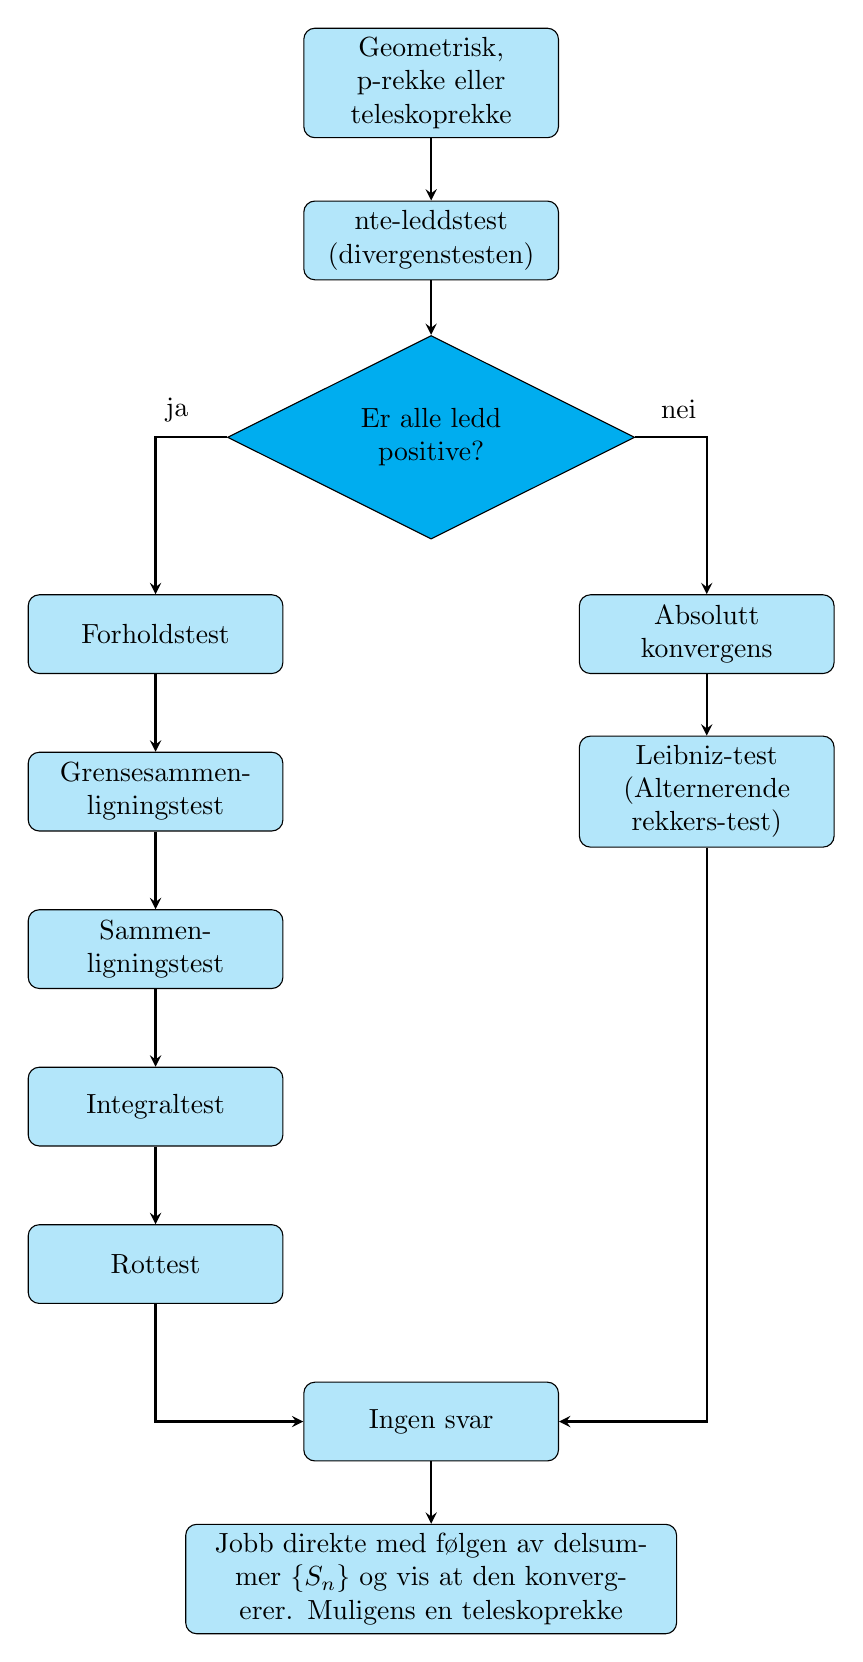
\begin{tikzpicture}[node distance=2cm, auto]
		\centering
		
	    \node (steg1) [prosess] {Geometrisk, p-rekke eller teleskoprekke};
		\node (steg2) [prosess, below of=steg1] {nte-leddstest (divergenstesten)};
		\node (valg1) [valg, below of=steg2, yshift= -0.5cm] {Er alle ledd positive?};
        \node (steg3) [prosess, right of=valg1, yshift=-2.5cm, xshift=1.5cm] {Absolutt konvergens};
        \node (steg4) [prosess, below of=steg3] {Leibniz-test (Alternerende rekkers-test)};
        \node (steg5) [prosess, left of=valg1, yshift=-2.5cm, xshift=-1.5cm] {Forholdstest};
        \node (steg6) [prosess, below of=steg5] {Grensesammen-ligningstest};
        \node (steg7) [prosess, below of=steg6] {Sammen-ligningstest};
        \node (steg8) [prosess, below of=steg7] {Integraltest};
        \node (steg9) [prosess, below of=steg8] {Rottest};
        \node (steg10) [prosess, below of=valg1, yshift=-10.5cm] {Ingen svar};
        \node (steg11) [prosess, below of=steg10, text width=6cm] {Jobb direkte med følgen av delsummer \(\left\lbrace S_n\right\rbrace \) og vis at den konvergerer. Muligens en teleskoprekke};
        
        \draw [arrow] (steg1) -- (steg2);
        \draw [arrow] (steg2) --  (valg1);
        \draw [arrow] (valg1) -| node[anchor=east,yshift=10pt]{nei}(steg3);
        \draw [arrow] (steg3) -- (steg4);
        \draw [arrow] (steg4) |- (steg10);
        \draw [arrow] (valg1) -| node[anchor=west,yshift=10pt]{ja} (steg5);
        \draw [arrow] (steg5) -- (steg6);
        \draw [arrow] (steg6) -- (steg7);
        \draw [arrow] (steg7) -- (steg8);
        \draw [arrow] (steg8) -- (steg9);
        \draw [arrow] (steg9) |- (steg10);
        \draw [arrow] (steg10) -- (steg11);
		\end{tikzpicture}
	}
\end{center}
		\newpage
		
		\section{Potensrekker}
		
		\begin{fmindef}[Potensrekke]
			En \textit{potensrekke} omkring \(x=a\) er en rekke på formen 
			\[\sum_{n=0}^{\infty}c_n(x-a)^n=c_0+c_1(x-a)+c_2(x-a)^2+c_3(x-a)^3+...,\]
			
			der \(x\) er en variabel, mens \(a\) og \(c_n\) er (reelle) konstanter. Vi kaller \(a\) og \(c_n\) for henholdsvis \textit{sentrum} og \textit{koeffisientene} til potensrekken. 
			
			En potensrekke omkring \(x=0\) har formen
			
			\[\sum_{n=0}^{\infty}c_nx^n=c_0+c_1x+c_2x^2+c_3x^3+...\]
		\end{fmindef}
		
		\begin{fteo}
			La \[\sum_{n=0}^{\infty}c_n(x-a)^n \]
			være en potensrekke. Da har vi tre muligheter
			\begin{enumerate}
				\item Potensrekken konvergerer for alle \(x\in \mathbb{R}. \)
				\item Potensrekken konvergerer bare for \(x=a\) (og er lik \(c_0\) siden \((x-a)^n=0\) når \(x=a\)).
				\item Potensrekken konvergerer for alle \(x\) i et endelig intervall \(I\) (og \(x=a\) er midtpunktet til dette intervallet).
			\end{enumerate}
		\end{fteo}
		
		
		\newpage
		
		\begin{fminset} 
			Teste en potensrekke for konvergens 
			
			\begin{enumerate}
				\item Bruk \textit{forholdstesten} eller \textit{rottesten} for å finne intervallet der rekken konvergerer absolutt. Ordinæt et åpent intervall
				\[|x-a|<R\hspace{32pt}\text{eller}\hspace{32pt}a-R<x<a+R\]
				\item Hvis intervallet av absolutt konvergens er endelig, test for konvergens eller divergens ved hvert endepunkt. Bruk sammenligningststen, Integraltesten, eller Leibniz-testen.
				\item Hvis intervallet for absolutt konvergens er \(a-R<x<a+R\), divergerer rekken for \(|x-a|>R\) (den konvergerer ikke en gang betinget) fordi nte ledd ikke nærmer seg null for de verdiene av \(x\).
			\end{enumerate}
			
		\end{fminset}
		
		\newpage
		
		\subsubsection{Oppgaver med løsningsforslag}
		
		Finn konvergeringsintervallet til rekkene
		
		\begin{enumerate}
			\item \(\displaystyle{\sum_{n=1}^{\infty}\dfrac{(3x-2)^n}{n}}\)
			
			Bruker forholdstest
			
			\begin{align*}
			\lim\limits_{n\rightarrow \infty}\left| \dfrac{(3x-2)^{\cancel{n}+1}}{n+1}\cdot \dfrac{n}{\cancel{(3x-2)^n}} \right| = \lim\limits_{n\rightarrow \infty}\left|  \dfrac{(3x-2)\cancel{n}}{\cancel{n}(1+\frac{1}{n})}\right|=\left|  3x-2 \right| <1
			\end{align*}
			
			\begin{align*}
			(3x - 2) &< 1		\\
			3x&<3			\\
			x&<1			
			\end{align*}
			\begin{align*}
			-(3x-2)&<1\\
			-3x+2&<1\\
			-3x&<1\\
			x&>\frac{1}{3}
			\end{align*}
			\[\underline{\underline{\frac{1}{3}<x<1}} \]
			\newpage
			\item \(\displaystyle{\sum_{n=1}^{\infty}\dfrac{(x-2)^n}{10^n}}\)
			
			Ser at dette er ei geometrisk rekke med \(r=\dfrac{x-2}{10}\). Slipper derfor å bruke forholdstesten. Skal løse likningen \(\lim\limits_{n\rightarrow \infty}\left| \dfrac{x-2}{10} \right|<1 \) , fordi \(|r|<1\) er betingelsen for at ei geometrisk rekke konvergerer
			
			\begin{align*}
			\left( \dfrac{x-2}{10}\right)  &<1\\
			x-2&<10 \\
			x&<12
			\end{align*}
			\begin{align*}
			-\left( \dfrac{x-2}{10}\right)&<1\\
			-x&<8\\
			x&>-8 
			\end{align*}
			\[\underline{\underline{-8<x<12}}\]
		\end{enumerate}
		

		
		\newpage
		
		\section{Taylor-rekker}
		
		\begin{fmindef}
			La \(f(x)\) være en funksjon som er uendelig mange ganger deriverbar i \(x=a\). 
			
			\textbf{Taylor-rekken} til \(f(x)\) i \(a\) definert ved
			
			
			\[P(x)=\sum_{n=0}^{\infty}\dfrac{f^{(n)}(a)}{n!}(x-a)^n\]
			\[=f(a)+f^{\prime}(a)(x-a)+\dfrac{f^{\prime \prime}(a)}{2!}(x-a)^2+\cdots+\dfrac{f^{(n)}(a)}{n!}(x-a)^n+\cdots.\]
		
			\textbf{Maclurin-rekken	} til \(f(x)\) er
			
			\[P(x)=\sum_{n=0}^{\infty} \dfrac{f^{(n)}(0)}{n!}x^n \]
			
			\[=f(0)+f^{\prime}(0)x+\dfrac{f^{\prime \prime}(0)}{2!}x^2+\cdots+\dfrac{f^{(n)}(0)}{n!}x^n+\cdots.\]
			
			som er \textit{taylor-rekken} når \(x=0\).
		\end{fmindef}
		
		\subsection{Taylor-polynom}
		
		Delsummene til \textit{Taylor-rekker} kalles \textit{Taylor-polynomer}. Polynomer er enkle å regne med, siden de bare involverer addisjon og multiplikasjon. Datamaskinen kan finne tilnærminger til kompliserte funksjoner ved hjelp av \textit{Taylor-polynomer}. 
		
		
		\begin{fmindef}
			Anta at \(f(x)\) er en funksjon som minst \(N\) ganger deriverbar i \(a\). Da definerer vi \textit{Taylor-polynomet} av \(N\)-te orden til \(f(x)\) i \(a\) ved
			\[P_N(x)=\overbrace{\underbrace{\underbrace{f(a)}_{P_0(x)}+f^{\prime}(a)(x-a)}_{P_1(x)}+\dfrac{f^{\prime \prime}(a)}{2!}(x-a)^2}^{P_2(x)}
			+\cdots+\dfrac{f^{(N)}(a)}{N!}(x-a)^N
			\]
			\[=\sum_{n=0}^{N}\dfrac{f^{(n)}(a)}{n!}(x-a)^n \]
		\end{fmindef}
		
		\newpage
		
		\subsection{Kjente maclaurinrekker}
		
		\begin{enumerate}
			\item \[e^x=1+x+\dfrac{x^2}{2!}+\dfrac{x^3}{3!}+\cdots=\sum_{n=0}^{\infty}\dfrac{x^n}{n!}\text{ for alle }x. \]
			\item
			\[cos(x)=1-\dfrac{x^2}{2!}+\dfrac{x^4}{4!}-\dfrac{x^6}{6!}+\cdots =\sum_{n=0}^{\infty}(-1)^n\dfrac{x^{2n}}{(2n)!} \text{ for alle }x. \]
			\item
			\[sin(x)=x-\dfrac{x^3}{3!}+\dfrac{x^5}{5!}-\dfrac{x^7}{7!}+\cdots=\sum_{n=0}^{\infty}(-1)^n\dfrac{x^{2n+1}}{(2n+1)!}\text{ for alle }x. \]
			\item
			\[ln(1+x)=x-\dfrac{x^2}{2}+\dfrac{x^3}{3}-\cdots =\sum_{n=1}^{\infty}(-1)^{n-1} \dfrac{x^n}{n} \text{ for }-1<x\leq 1. \]
			\item \[\dfrac{1}{1-x}=1+x+x^2+x^3+x^4+\cdots=\sum_{n=0}^{\infty}x^n \text{ for }-1<x< 1.\]
		\end{enumerate}
		
		\newpage
		
		\subsection{Nyttige følger}
		\textbf{Oddetall}
		\(\left\lbrace 2n+1 \right\rbrace_{n=1}^{\infty}\)
		\[1,3,5,7,\cdots,2n+1,\cdots\]		
		
		\textbf{Partall} \(\left\lbrace 2n\right\rbrace_{n=0}^{\infty}\)
		\[0,2,4,6,\cdots,2n,\cdots\]
		
		\(\left\lbrace n! \right\rbrace_{n=0}^{\infty}\)
		\[1,1,2,6,24,\cdots \]
		
		\(\left\lbrace 2n! \right\rbrace_{n=0}^{\infty}\)
		\[2,2,4,12,48,\cdots \]
		 
		\(\left\lbrace 3n! \right\rbrace_{n=0}^{\infty}\)
		\[3,3,6,18,72,\cdots \]
		 
    	\(\left\lbrace (-1)^{n} \right\rbrace_{n=0}^{\infty}\)
	    \[1,-1,1,-1,\cdots\]
		  
		\(\left\lbrace (1+x)^{-n-1} \right\rbrace_{n=0}^{\infty}\)
		\[(1+x)^{-1},(1+x)^{-2},(1+x)^{-3},(1+x)^{-4},\cdots\]
		\newpage
		
		
		\subsubsection{Oppgaver med løsningsforslag}
		
		\begin{enumerate}
			\item Finn \textit{Taylor-polynomet} til \(f(x)\) av tredje grad, om x=a. \[f(x)=\frac{1}{x}, \,\,\,\,\, a=2\]
			
			Løsning:
			
			\[f(x)=\frac{1}{x},\hspace{16pt} f^{\prime}(x)=-\frac{1}{x^2} ,\hspace{16pt} f^{\prime \prime} (x)\frac{2}{x^3},\hspace{16pt} f^{\prime \prime \prime}(x)=-\frac{6}{x^4}\]
			
			Setter inn \(a=2\)
			
			\[f(2)=\frac{1}{2},\hspace{16pt} f^{\prime}(2)=-\frac{1}{4} ,\hspace{16pt} f^{\prime \prime} (2)\frac{1}{4},\hspace{16pt} f^{\prime \prime \prime}(2)=-\frac{3}{8}\]
			
			Setter inn i formelen
			\begin{align*}
			P_3(x)&=f(2)+f^{\prime}(2)(x-2)+\dfrac{f^{\prime \prime}(2)}{2!}(x-2)^2+\frac{f^{\prime \prime \prime
				}(2)}{3!}(x-2)^3\\
			&=\frac{1}{2}+\left( -\frac{1}{4}\right) (x-2)+\frac{\frac{1}{4}}{2}(x-2)^2+\frac{-\frac{3}{8}}{6}(x-2)^3\\
			&=\underline{\underline{\frac{1}{2}-\frac{1}{4}(x-2)+\frac{1}{8}(x-2)^2-\frac{1}{16}(x-2)^3}}
			\end{align*}
			
			\item Finn \textit{Maclaurin-rekken} til \(f(x)=e^x\)
			
			Løsning:
			
			\[f(x)=e^x \hspace{16pt}f^{\prime}(x)=e^x \hspace{16pt}f^{\prime \prime}(x)=e^x \hspace{16pt} f^{\prime \prime \prime}(x)=e^x \]
			
			\[f(0)=1 \hspace{16pt}f^{\prime}(0)=1 \hspace{16pt}f^{\prime \prime}(0)=1 \hspace{16pt} f^{\prime \prime \prime}(0)=1\hspace{10pt} \Rightarrow \hspace{10pt}f^n(0)=1 \]
			
			Maclurin-rekken til \(f(x)\) er \(\sum_{n=0}^{\infty} \dfrac{f^{(n)}(0)}{n!}x^n \). Så vi kan sette \(f^n(0)=1 \) rett inn i formelen, og vi får
			
			\[e^x=\sum_{n=0}^{\infty}\dfrac{x^n}{n!}=1+x+\dfrac{x^2}{2!}+\dfrac{x^3}{3!}+\cdots. \]
			
			\newpage
			
			\item Finn \textit{Maclaurin-rekken} til \(f(x)=cos\,x\)
			
			Løsning:
			\[f(x)=cos\,x \hspace{16pt} f^{\prime}(x)=-sin\,x \hspace{16pt} f^{\prime \prime}(x)=-cos\,x \hspace{16pt} f^{\prime \prime \prime}(x)=sin\,x \hspace{16pt} f^{(4)}(x)=cos\,x \]
			\[f(0)=1 \hspace{16pt} f^{\prime}(0)=0 \hspace{16pt} f^{\prime \prime}(0)=-1 \hspace{16pt} f^{\prime \prime \prime}(0)=0 \hspace{16pt} f^{(4)}(0)=1 \]
			
			\[P(x)=\sum_{n=0}^{\infty} \dfrac{f^{(n)}(0)}{n!}x^n=1-\frac{x^2}{2!}+\frac{x^4}{4!}-\cdots=\sum_{n=0}^{\infty} (-1)^n\frac{x^{2n}}{(2n)!} \]
			
			\item Finn \textit{Maclaurin-rekken} til \(f(x)=sin\,x\)
			
			Løsning:
			\[f(x)=sin\,x \hspace{16pt} f^{\prime}(x)=cos\,x \hspace{16pt} f^{\prime \prime}(x)=-sin\,x \hspace{16pt} f^{\prime \prime \prime}(x)=-cos\,x \hspace{16pt} f^{(4)}(x)=sin\,x \]
			\[f(0)=0 \hspace{16pt} f^{\prime}(0)=1 \hspace{16pt} f^{\prime \prime}(0)=0 \hspace{16pt} f^{\prime \prime \prime}(0)=-1 \hspace{16pt} f^{(4)}(0)=0 \]
			
			\[P(x)=\sum_{n=0}^{\infty} \dfrac{f^{(n)}(0)}{n!}x^n=
			x-\dfrac{x^3}{3!}+\dfrac{x^5}{5!}-\cdots=
			\sum_{n=0}^{\infty}(-1)^n\dfrac{x^{2n+1}}{(2n+1)!}  \]
			
			\item Finn \textit{Maclaurin-rekken} til \(f(x)=ln(1+x)\)
			
			Løsning:
			\begin{align*}
			&f(x)=ln(1+x) \hspace{16pt} f^{\prime}(x)=\dfrac{1}{1+x} \hspace{16pt} f^{\prime \prime}(x)=-\dfrac{1}{(1+x)^2} \hspace{16pt} \\ 
			&f^{\prime \prime \prime}(x)=\dfrac{2	}{(1+x)^3} \hspace{16pt} f^{(4)}(x)=-\dfrac{6}{(1+x)^4}
			\hspace{16pt} f^{(5)}=\dfrac{18}{(1+x)^5}
			\end{align*}
			\begin{align*}
			&f(0)=0 \hspace{16pt} f^{\prime}(0)=1 \hspace{16pt} f^{\prime \prime}(x)=-1 \hspace{16pt} \\ 
			&f^{\prime \prime \prime}(x)=2 \hspace{16pt} f^{(4)}(x)=-6
			\hspace{16pt} f^{(5)}=18
			\end{align*}
			
			\begin{align*}
			P(x)&=\sum_{n=0}^{\infty}
			 \dfrac{f^{(n)}(0)}{n!}x^n=
			\underbrace{0}_{n=0}+\underbrace{x}_{n=1}\underbrace{-\dfrac{x^2}{2!}}_{n=2}\underbrace{+\dfrac{2!x^3}{3!}}_{n=3}\underbrace{-\dfrac{3!x^4}{4!}}_{n=4}+\cdots\\
			&x-\dfrac{x^2}{2!}+\dfrac{\cancel{2!}x^3}{3\cdot \cancel{2}}-\dfrac{\cancel{3!}x^4}{4\cdot \cancel{3!}}+\cdots = x-\dfrac{x^2}{2}+\dfrac{x^3}{3}-\dfrac{x^4}{4}+\cdots\\
			&=\sum_{n=0}^{\infty} (-1)^{n-1} \dfrac{x^{n}}{n}
			\end{align*}
			
			\newpage
			
			\item Finn \textit{Maclaurin-rekken} til \(f(x)=e^{-x}\)
			
		    Løsning:
		    
		    Vi vet at \(e^x=\displaystyle{ \sum_{n=0}^{\infty}}\dfrac{x^n}{n!}\) og kan derfor sette \(-x\) for \(x\)
		    
		    \begin{align*}
		    e^{-x}&=\sum_{n=0}^{\infty}\dfrac{(-x)^n}{n!}=1+(-x)+\dfrac{(-x)^2}{2!}+\dfrac{(-x)^3}{3!}+\dfrac{(-x)^4}{4!}+\cdots\\
		    &=1-x+\dfrac{x^2}{2!}-\dfrac{x^3}{3!}+\dfrac{x^4}{4!}-\cdots=\sum_{n=0}^{\infty}(-1)^n\dfrac{x^n}{n!}
		    \end{align*}
		    
		    \item Finn \textit{Maclaurin-rekken} til \(f(x)=sin\left( \frac{x}{2}\right) \)
		    
		    Løsning:
		    
		     Vi vet at \(sin\,x=\displaystyle{\sum_{n=0}^{\infty}(-1)^n\dfrac{x^{2n+1}}{(2n+1)!}} \) og kan derfor sette inn \(\dfrac{x}{2}\) for \(x\)
		     
		     \begin{align*}
		     sin\left( \dfrac{2}{x} \right) &= \sum_{n=0}^{\infty}(-1)^n \dfrac{\left( \frac{x}{2} \right)^{2n+1} }{(2n+1)!}=\sum_{n=0}^{\infty}(-1)^n \dfrac{ \frac{x^{2n+1}}{2^{2n+1}} }{(2n+1)!}\\
		     &=\sum_{n=0}^{\infty}(-1)^n\dfrac{x^{2n+1}}{2^{2n+1}(2n+1)!}=\dfrac{x}{2}-\dfrac{x^3}{2^3\cdot 3!}+\dfrac{x^5}{2^5\cdot 4!}-\cdots
		     \end{align*}
			
		\end{enumerate}
		
		\newpage
		
		\section{Trigonometriske rekker}
			
		\subsection{Egenskaper til cosinus og sinus (jevn og odde)}
		
		
		\subsubsection{Cosinus}
		\label{sec:EgenskaperCos}
		
		Funksjonen \(f(x)=\cos x\) er en \textbf{jevn} funksjon. Det vil si at den er symmetrisk om \textbf{y-aksen}.
		
		Vi har at \[\cos(-x)=\cos(x) \]
		
		og derfor er 
		
		\[\int\limits_{-\pi}^{\pi}\cos \theta \,d\theta = 0  \]
		
		Vi kan se at integralet må være \(0\) hvis vi ser på kurven \(y=\cos x  \) for \(x=-\pi\) til \(x=\pi \)
		
		\begin{figure}[!ht]
			\centering
			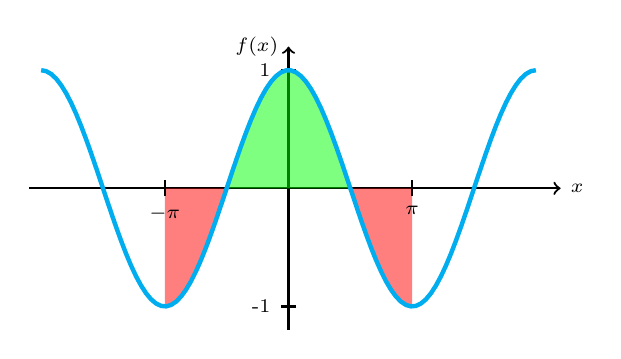
\begin{tikzpicture}[xscale=0.5,yscale=1.5]    				\begin{scope}[thick,font=\scriptsize]
			
			%Background
			
			
			
			% Axes:
			% Are simply drawn using line with the `->` option to make them arrows:
			% The main labels of the axes can be places using `node`s:
			\draw [->] (-3.1415*2.1,0) -- (3.1415*2.2,0) node [right] {\(x\)};
			\draw [->]  (0,-1.2) -- (0,1.2) node [left] {\(f(x)\)};
			
			\fill [red, domain=-3.1415:-1, samples=100, opacity=0.5] (-3.1415,0)  -- plot (\x, {cos(deg(\x))}) -- (-3.1415/2,0);
			
			\fill [red, domain=3.1415:1, samples=100, opacity=0.5] (3.1415,0)  -- plot (\x, {cos(deg(\x))}) -- (3.1415/2,0);
			
			\fill [green, domain=-3.1415/2:3.1415/2, samples=100, opacity=0.5] (-3.1415/2,0)  -- plot (\x, {cos(deg(\x))}) -- (3.1415/2,0);
			
			% Axes labels:
			% Are drawn using small lines and labeled with `node`s. The placement can be set using options
			% Single
			% If you only want a single label per axis side:
			
			\draw (0.2,-1) -- (-0.2,-1) node [left] {-1};
			\draw (0.2,1) -- (-0.2,1) node [left] {1};
			
			\draw (3.1415,0.2/3) -- (3.1415, -0.2/3) node [below] {\(\pi \)};
			\draw (-3.1415,0.2/3) -- (-3.1415, -0.2/3) node [below] {\(-\pi \)};
			
			\draw[cyan, ultra thick, domain= -3.1415*2:3.1415*2, samples=100] plot (\x, {cos(deg(\x))});
			
			\end{scope}
			
			\end{tikzpicture}
			\caption{ Integralet av \(y=\cos x \) for \(-\pi \leq x \leq \pi \)}
		\end{figure}
		
		Den røde "negative" delen av grafen og den grønne "positive" delen av grafen blir kanselerer hverandre ut. Summen blir 0.
		
		\newpage
		
		\subsubsection{Sinus}
		\label{sec:EgenskaperSin}
		Funksjonen \(f(x)=\sin x \) er en \textbf{odde} funksjon. Det vil si at den er symmetrisk om \textbf{origo}. 
		Vi har at \[\sin(-x)=- \sin(x) \]
		
		og derfor 
		
		\[\int\limits_{-\pi}^{\pi} \sin \theta \, d\theta =0 \]
		
		Igjen ser vi hvorfor illustrert i grafen under.
		
		\begin{figure}[!ht]
			\centering
			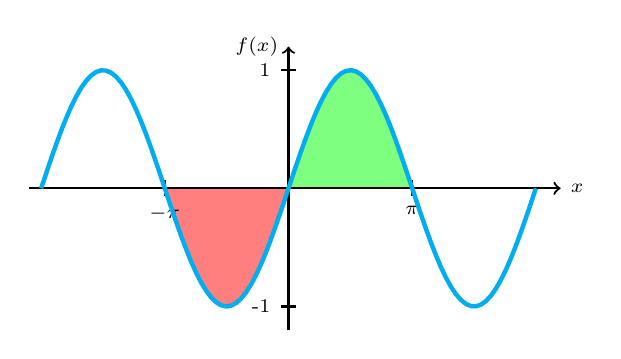
\begin{tikzpicture}[xscale=0.5,yscale=1.5]    				\begin{scope}[thick,font=\scriptsize]
			
			%Background
			
			\fill [red, domain=-3.1415:0, samples=100, opacity=0.5] (-3.1415,0)  -- plot (\x, {sin(deg(\x))}) -- (0,0);
			
			\fill [green, domain= 0:3.1415, samples=100, opacity=0.5] (0,0)  -- plot (\x, {sin(deg(\x))}) -- (3.1415,0);
			
			% Axes:
			% Are simply drawn using line with the `->` option to make them arrows:
			% The main labels of the axes can be places using `node`s:
			\draw [->] (-3.1415*2.1,0) -- (3.1415*2.2,0) node [right] {\(x\)};
			\draw [->]  (0,-1.2) -- (0,1.2) node [left] {\(f(x)\)};
			
			% Axes labels:
			% Are drawn using small lines and labeled with `node`s. The placement can be set using options
			% Single
			% If you only want a single label per axis side:
			
			\draw (0.2,-1) -- (-0.2,-1) node [left] {-1};
			\draw (0.2,1) -- (-0.2,1) node [left] {1};
			
			\draw (3.1415,0.2/3) -- (3.1415, -0.2/3) node [below] {\(\pi \)};
			\draw (-3.1415,0.2/3) -- (-3.1415, -0.2/3) node [below] {\(-\pi \)};
			
			\draw[cyan, ultra thick, domain= -3.1415*2:3.1415*2, samples=100] plot (\x, {sin(deg(\x))});
			
			\end{scope}
			
			\end{tikzpicture}
			\caption{ Integralet av \(y=\sin x \) for \(-\pi \leq x \leq \pi \)}
			
		\end{figure}
		
		Igjen ser vi at den negative røde delen er like stor som den grønne positive delen. Summen blir 0.
		
		\newpage
		
		\subsection{Flere hele \(\pi \) for cosinus og sinus}
		
		\subsubsection{Cosinus}
		
		Vi har funksjonen \(y=\cos x \)
		
		\begin{figure}[!ht]
			\centering
			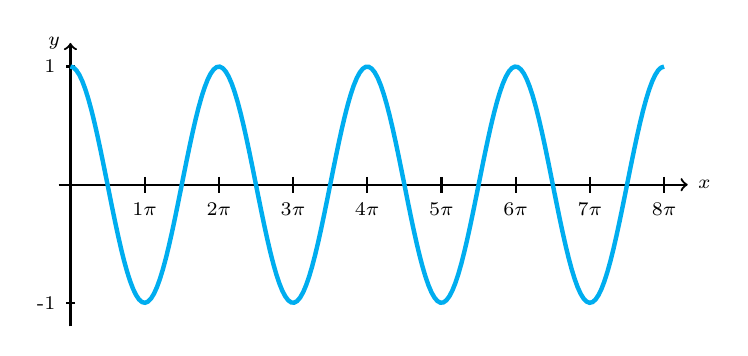
\begin{tikzpicture}[xscale=0.3,yscale=1.5]    				\begin{scope}[thick,font=\scriptsize]
			
			% Axes:
			% Are simply drawn using line with the `->` option to make them arrows:
			% The main labels of the axes can be places using `node`s:
			\draw [->] (-0.5,0) -- (3.1415*8+1,0) node [right] {\(x\)};
			\draw [->]  (0,-1.2) -- (0,1.2) node [left] {\(y\)};
			
			% Axes labels:
			% Are drawn using small lines and labeled with `node`s. The placement can be set using options
			% Single
			% If you only want a single label per axis side:
			
			\draw (0.2,-1) -- (-0.2,-1) node [left] {-1};
			\draw (0.2,1) -- (-0.2,1) node [left] {1};
			
			\foreach \n in {1,...,8}
			{
				\draw (3.1415*\n,0.2/3) -- (3.1415*\n, -0.2/3) node [below] { \n\(\pi \)};
			}
			
			\draw[cyan, ultra thick, domain= 0:3.1415*8, samples=200] plot (\x, {cos(deg(\x))});
			
			\end{scope}
			
			\end{tikzpicture}
			\caption{ Kurven \(y=\cos x\) for \(0 \leq x \leq 8\pi \)}
		\end{figure}
		
		\bgroup
		\def\arraystretch{1.5}
		\begin{tabular}{ll}
			\(\cos(2n\pi)=1 \)& \(\hspace{16pt}\text{for} \,\, n=0,1,2,3,\cdots,(\text{alle heltall}) \) \\ 
			\(\cos\left[ \left( 2n-1\right)\pi  \right]=-1  \)& \(\hspace{16pt}\text{for} \,\, n=0,1,2,3,\cdots,(\text{alle heltall})\) \\
			\(\cos(n\pi)=(-1)^n \)& \(\hspace{16pt}\text{for} \,\, n=0,1,2,3,\cdots,(\text{alle heltall})\) \\ 
		\end{tabular} 
		\egroup
		
		
	    \subsubsection{Sinus}
		
		
		Vi har funksjonen \(y=\sin x \)
		
		\begin{figure}[!ht]
			\centering
			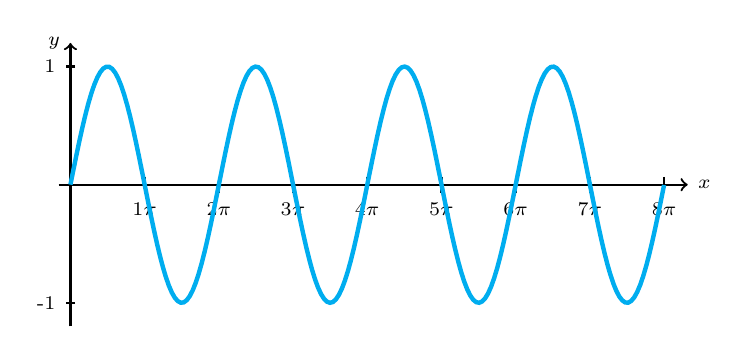
\begin{tikzpicture}[xscale=0.3,yscale=1.5]    				\begin{scope}[thick,font=\scriptsize]
			
			% Axes:
			% Are simply drawn using line with the `->` option to make them arrows:
			% The main labels of the axes can be places using `node`s:
			\draw [->] (-0.5,0) -- (3.1415*8+1,0) node [right] {\(x\)};
			\draw [->]  (0,-1.2) -- (0,1.2) node [left] {\(y\)};
			
			% Axes labels:
			% Are drawn using small lines and labeled with `node`s. The placement can be set using options
			% Single
			% If you only want a single label per axis side:
			
			\draw (0.2,-1) -- (-0.2,-1) node [left] {-1};
			\draw (0.2,1) -- (-0.2,1) node [left] {1};
				
			\foreach \n in {1,...,8}
			{
				\draw (3.1415*\n,0.2/3) -- (3.1415*\n, -0.2/3) node [below] { \n\(\pi \)};
			}
			
			\draw[cyan, ultra thick, domain= 0:3.1415*8, samples=200] plot (\x, {sin(deg(\x))});
			
			\end{scope}
			
			\end{tikzpicture}
			\caption{ Kurven \(y=\sin x\) for \(0 \leq x \leq 8\pi \)}
		\end{figure}
			Fra grafen (eller ved å bruke kalkulator), finner vi ut at: \bigskip
	
	
	        \bgroup
	        \def\arraystretch{1.5}
			\begin{tabular}{ll}
			\(\sin(n\pi)=0\) 	& \(\hspace{16pt}\text{for} \,\, n=0,1,2,3,\cdots,(\text{alle heltall}) \) \\ 
			\(sin\left( \dfrac{(2n-1)\pi}{2}\right)=(-1)^{n+1} \)	& \(\hspace{16pt}\text{for} \,\, n=0,1,2,3,\cdots,(\text{alle heltall})\) \\ 
			\end{tabular} 
			\egroup
			
			
			
		\newpage
		
		\subsection{Noen nyttige integraler}
		
		De neste integralene kan vi finne ved å bruke delvis integrasjon. De blir brukt en del i Fourier-rekke oppgaver. Disse er også lagt ved på formelark.
		
		\begin{enumerate}
			\item \[\int t \cos (nt) \,dt=\dfrac{\cos (nt)}{n^2}+\dfrac{t \sin (nt)}{n}=\dfrac{1}{n^2}(\cos (nt) +nt \sin (nt)) \]
			\item
			\[\int t^2 \cos(nt)\,dt=-2\dfrac{\sin(nt)}{n^3}+2\dfrac{t\cos(nt)}{n^2}+\dfrac{t^2\sin(nt)}{n} \]
			\item 
			\[\int t \sin (nt) \,dt=\dfrac{\sin (nt)}{n^2}-\dfrac{t \cos (nt)}{n}=\dfrac{1}{n^2}(\sin (nt) - nt \cos (nt)) \]
			\item
			\[\int t^2 \sin(nt)\,dt=2\dfrac{\cos(nt)}{n^3}+2\dfrac{t\sin(nt)}{n^2}-\dfrac{t^2\cos(nt)}{n} \]
		\end{enumerate}
		
		
		
		\newpage
		
		\subsection{Periodiske funksjoner}
				
		\begin{fmindef}
			En funksjon \(f(x)\) er \textbf{periodisk} med \textbf{perioden} \(T\) når 
			\[f(x+T)=f(x) \hspace{16pt} \text{for alle verdier av x.} \]
			Prinsipalperioden til \(f(x)\) er den minste \(T>0\) for at dette skal gjelde.
		\end{fmindef}
		
		Eksempel på periodeiske funksjoner
		
		\(f(x)=\sin x \) 
		
		\begin{figure}[!ht]
			\centering
			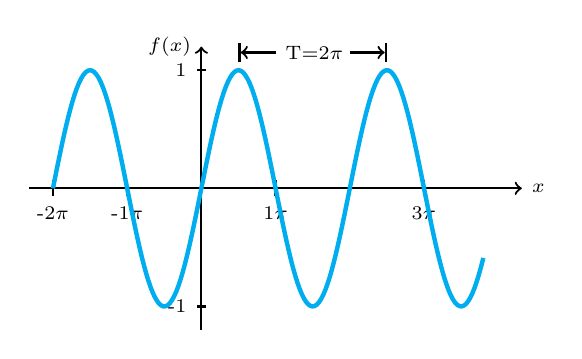
\begin{tikzpicture}[xscale=0.3,yscale=1.5]    				\begin{scope}[thick,font=\scriptsize]
			
			% Axes:
			% Are simply drawn using line with the `->` option to make them arrows:
			% The main labels of the axes can be places using `node`s:
			\draw [->] (-3.1415*2-1,0) -- (3.1415*4+1,0) node [right] {\(x\)};
			\draw [->]  (0,-1.2) -- (0,1.2) node [left] {\(f(x)\)};
			
			% Axes labels:
			% Are drawn using small lines and labeled with `node`s. The placement can be set using options
			% Single
			% If you only want a single label per axis side:
			
			\draw (0.2,-1) -- (-0.2,-1) node [left] {-1};
			\draw (0.2,1) -- (-0.2,1) node [left] {1};
			
			\foreach \n in {-2,-1,1,...,4}
			{
				\draw (3.1415*\n,0.2/3) -- (3.1415*\n, -0.2/3) node [below] { \n\(\pi \)};
			}
			
			\draw[cyan, ultra thick, domain= -2*3.1415:3.1415*3.8, samples=200] plot (\x, {sin(deg(\x))});
			
			
			\draw[|<-] (3.1415/2,1.15) -- (3.1415*2/2,1.15);
			
			\draw[|<-] (3.1415*5/2,1.15) -- (3.1415*4/2,1.15) node [pos =0.9,left] {T=2\(\pi \)};
		
			\end{scope}
			
			\end{tikzpicture}
			\caption{ Kurven \(y=\sin x\) med periode \(=2\pi\)}
		\end{figure}
		
		For \(f(x)=\sin x\), har vi: \(f(x)=f(x+2\pi).\) perioden er \(2\pi \) 
		\bigskip
		
		Firkantbølge, periode=4
		
		\begin{figure}[!ht]
			\centering
			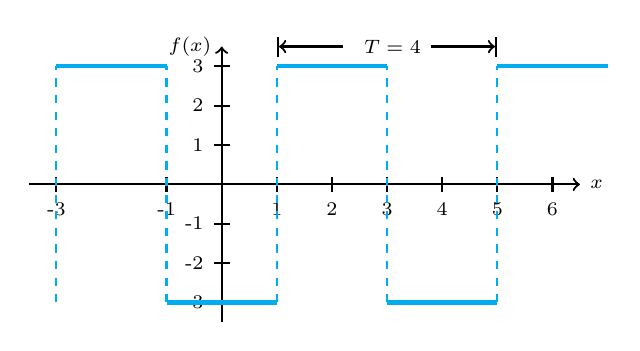
\begin{tikzpicture}[xscale=0.7,yscale=0.5]    				\begin{scope}[thick,font=\scriptsize]
			
			% Axes:
			% Are simply drawn using line with the `->` option to make them arrows:
			% The main labels of the axes can be places using `node`s:
			\draw [->] (-3.5,0) -- (6.5,0) node [right] {\(x\)};
			\draw [->]  (0,-3.5) -- (0,3.5) node [left] {\(f(x)\)};
			
			% Axes labels:
			% Are drawn using small lines and labeled with `node`s. The placement can be set using options
			% Single
			% If you only want a single label per axis side:
						
			\foreach \n in {-3,-2,-1,1,2,3}
			{
				\draw (0.2/1.4,\n) -- (-0.2/1.4, \n) node [left] { \n};
				}
	
			\foreach \n in {-3,-1,1,2,...,6}
			{
					\draw (\n,0.2) -- (\n, -0.2) node [below] { \n};
			}
			
			\draw[cyan, ultra thick, domain=-3:-1] plot (\x,3);
			\draw[cyan, ultra thick, domain=-1:1] plot (\x,-3);
			\draw[cyan, ultra thick, domain=1:3] plot (\x,3);
			\draw[cyan, ultra thick, domain=3:5] plot (\x,-3);
			\draw[cyan, ultra thick, domain=5:7] plot (\x,3);
			
			\draw[cyan, dashed, domain=-3:3,variable=\y] plot (-3,\y);
			\draw[cyan, dashed, domain=-3:3,variable=\y] plot (-1,\y);
			\draw[cyan, dashed, domain=-3:3,variable=\y] plot (1,\y);
			\draw[cyan, dashed, domain=-3:3,variable=\y] plot (3,\y);
			\draw[cyan, dashed, domain=-3:3,variable=\y] plot (5,\y);
				
			\draw[|<-] (1,3.5)--(2.2,3.5);
			\draw [|<-] (5,3.5)--(3.8,3.5)node [left] {\(T=4\)};
			
			\end{scope}
			
			\end{tikzpicture}
			\caption{Periodisk firekant bølge funksjon}
		\end{figure}
		
		For denne funksjonene har vi:
		
		\[ f(x)=-3 \text{ for } -1\leq x \text{ og }3 \text{ for } 1\leq x \leq 3 \]
		\[f(x)=f(x+4) \]
		
		\newpage
		
		\begin{mitteks}
			Lag en skisse av følgende funksjon \[
			f(t)=
			\begin{cases}
			t \hspace{8pt} &\text{for} \hspace{12pt} 0\leq t < \pi \\
			t-\pi \hspace{8pt} &\text{for} \hspace{12pt} \pi \leq t <2\pi 
			\end{cases}
			\]
		\end{mitteks}
		
		\begin{figure}[!ht]
			\centering
			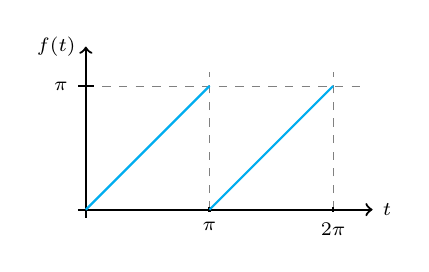
\begin{tikzpicture}[xscale=0.5,yscale=0.5]    				\begin{scope}[thick,font=\scriptsize]
			
			\draw[step=3.1415,gray, very thin, dashed] (0,0) grid (7,3.5);
			% Axes:
			% Are simply drawn using line with the `->` option to make them arrows:
			% The main labels of the axes can be places using `node`s:
			\draw [->] (-0.2,0) -- (3.1415*2+1,0) node [right] {\(t\)};
			\draw [->]  (0,-0.2) -- (0,3.1415+1) node [left] {\(f(t)\)};
			
			% Axes labels:
			% Are drawn using small lines and labeled with `node`s. The placement can be set using options
			% Single
			% If you only want a single label per axis side:
			
			
			\draw (0.2,3.1415) -- (-0.2,3.1415) node [left] {\(\pi \)};
			
			
			
		    \draw (3.1415*1,0.2/3) -- (3.1415*1, -0.2/3) node [below] {\(\pi \)};
		    \draw (3.1415*2,0.2/3) -- (3.1415*2, -0.2/3) node [below] {\(2\pi \)};
			
		
			\draw[cyan , thick, domain=0:3.1415] plot (\x,\x);
			\draw[cyan , thick, domain=0:3.1415] plot (\x+3.1415,\x);
			
			
			
			
			\end{scope}
			
			\end{tikzpicture}
		
		\end{figure}
		\newpage
		
		\subsection{Fourier-rekker}
		
		\begin{fmindef}
			En trigonometrisk rekke med perioden \(T\) er en rekke på formen
			\[a_0+\sum_{n=1}^{\infty} \left( a_n \cos \dfrac{2\pi n x}{T}+b_n\sin \frac{2\pi n x }{T} \right). \]
		\end{fmindef}
		
		\begin{fmindef}
			La \(f\) være en periodisk funksjon med perioden \(T\), og la \(L=\frac{T}{2}\). Da er fourierrekken til \(f\)
			\[a_0+\sum_{n=1}^{\infty}\left(a_n \cos \left( \frac{n\pi x}{L} \right)+b_n \sin \left( \frac{n\pi x}{L} \right)   \right).  \]
		
		Her er 
		
		\[a_0=\dfrac{1}{2L}\int\limits_{-L}^{L} f(x) \, dx, \]
		
		\[a_n=\dfrac{1}{L}\int\limits_{-L}^{L} f(x)\cos \left( \frac{n\pi x}{L} \right) \,dx, \]
		
		\[b_n=\dfrac{1}{L}\int\limits_{-L}^{L}f(x)\sin \left( \dfrac{n\pi x}{L} \right) \, dx.  \]
     	\end{fmindef}
		\newpage
		
		Vi skal tilnærme funksjoner definert på intervallet \([-\pi , \, \pi] \)
		
		\begin{fmindef}
			En \textit{trigonometrisk rekke } med perioden \(2\pi \) er en rekke på formen
			\[a_0+\sum_{n=1}^{\infty}(a_n\cos nx+b_n\sin nx). \]
		\end{fmindef}
		
		\begin{fmindef}
			La \(f(x)\) være en funksjon definert for \(x\in[-\pi,\,\pi]\). Forutsatt at integralet eksisterer, definer, definerer vi \textit{Fourier-koeffisiente-ne} ved
			
			\[a_0=\dfrac{1}{2\pi}\int\limits_{-\pi}^{\pi}  f(x)\,dx \] 
			
			\[a_n=\dfrac{1}{\pi}\int\limits_{-\pi}^{\pi}  f(x)\cos nx \,dx \]
			
			\[b_n=\dfrac{1}{\pi}\int\limits_{-\pi}^{\pi}  f(x)\sin nx \,dx \]
			
			\textit{Fourier-rekken} til \(f(x)\) er defienert som den trigonometriske rekken
			
			\[Ff(x)=a_0 + \sum_{n=1}^{\infty}(a_n\cos nx + b_n \sin nx),\]
			
			der koeffisientene er gitt ved formelene ovenfor.  
		\end{fmindef}
		
		\newpage
		
		\subsection{Fourier-rekker av jevne funksjoner}
		
		For en \textbf{jevn} funksjon \(f(x)\), definert for \(-L\) til \(L\), har vi følgende nyttige snarvei.
		
		Siden \[b_n=\dfrac{1}{L}\int\limits_{-L}^{L}f(x)\sin\left(\dfrac{n\pi x}{L} \right)\, dx   \]
		og \(f(x)\) er jevn, betyr det at integralet vil ha verdi 0. (Som er forklart i \ref{sec:EgenskaperCos}).
		
		Så for en Fourier Rekke for en jevn funksjon, har koeffisienten \(b_n\) verdi null.
		
		\[b_n=0\]
		
		
		Så vi trnger berre å regne ut \(a_0\) og \(a_n\).
		
		En \textbf{jevn} funksjon har bare \textbf{cosinus} ledd i sin Fourier ekspansjon.
		
		\begin{fmindef}
			Fourier-rekke til en \textbf{jevn} funksjon
			
			\[a_0=\dfrac{1}{L}\int\limits_{0}^{L} f(x) \, dx, \]
			
			\[a_n=\dfrac{2}{L}\int\limits_{0}^{L} f(x)\cos \left( \frac{n\pi x}{L} \right) \,dx, \]
			
			\[Ff(x)=a_0+\sum_{n=1}^{\infty}a_n\dfrac{\cos (n\pi x)}{L} \]
		\end{fmindef}
	   	
		
		\newpage


		\subsection{Fourier-rekker av odde funksjoner}
		
		For en \textbf{odde} funksjon \(f(x)\), definert for \(-L\) til \(L\), har vi følgende nyttige snarvei.
		
		Siden \[a_n=\dfrac{1}{L}\int\limits_{-L}^{L}f(x)\cos\left(\dfrac{n\pi x}{L} \right)\, dx   \]
		
		Så \textbf{null koeffiesientene} i dette tilfellet er: \[a_0=0 \,\,\text{ og } \,\, a_n=0\]
		
		Så vi trenger berre å regne ut \[b_n\]
		
		En \textbf{odde} funksjon har bare \textbf{sinus} ledd i sin Fourier ekspansjon.
		
		\begin{fmindef}
			Fourier-rekke til en \textbf{odde} funksjon
			
			\[b_n=\dfrac{2}{L}\int\limits_{0}^{L}f(x)\sin \left( \dfrac{n\pi x}{L} \right) \, dx \]
			
			\[Ff(x)=\sum_{n=1}^{\infty}b_n \sin \left( \dfrac{n\pi x}{L} \right)\, dx.  \]
		\end{fmindef}
		
		
		
		\newpage		
		
		\subsection{Halvperiodiske utvidelser}
		
		Vi tar for oss halvperiodiske utvidelser. Vi tenker oss at intervallet, \(0 \) til \(L\) er en halv periode, og at vi har en funksjon \(f(x)\) definert for \(x\) i dette intervallet. Uten tillegsopplysninger finnes ingen entydig måte å utvide \(f(x)\) til en funksjon med perioden \(T=2L\). Om vi spesifiserer en symmetri - at resultatet skal være enten jevn eller en odde funksjon - blir utvidelsen veldefinert:
		
		
		\subsubsection{Jevn funskjon}
		
		La \(f(x)\) være definert i intervallet \(\langle 0,L \rangle\)
		
		\[Ff(x)=a_0+\sum_{n=1}^{\infty}a_n\dfrac{\cos (n\pi x)}{L} \]
		
		\[a_0=\dfrac{1}{L}\int\limits_{0}^{L} f(x) \, dx, \]
		
		\[a_n=\dfrac{2}{L}\int\limits_{0}^{L} f(x)\cos \left( \frac{n\pi x}{L} \right) \,dx, \]
		
		\[b_n=0\]
		
		\subsubsection{Odde funskjon}
		
		La \(f(x)\) være definert i intervallet \(\langle 0,L \rangle\)
		
		\[Ff(x)=\sum_{n=1}^{\infty}b_n \sin \left( \dfrac{n\pi x}{L} \right)\, dx.  \]
		
		\[b_n=\dfrac{2}{L}\int\limits_{0}^{L}f(x)\sin \left( \dfrac{n\pi x}{L} \right) \, dx \]
		
		\[a_0=0,\,\,\,\,a_n=0\]
		
		\newpage
		
		\subsection{Konvergens for Fourier-rekker}
		
		\begin{fminset}[Fouriers setning]
			
			La \(f(x)\) være en periodisk funksjon med perioden \(T\) som er slik at både \(f(x)\) og dens deriverte \(f^{\prime}(x)\) er stykkevis kontinuerlig. Da konvergerer Fourier-rekken \(Ff(x)\) mot \(f(x)\) i alle de punkter \(x\) der \(f\) er kontinuerlig \[Ff(x)=f(x)\] 
			, og mot
			\[\frac{1}{2}\left[ \lim\limits_{n\rightarrow a^{+}}f(x) + \lim\limits_{n\rightarrow a^{-}}f(x) \right] \]
			forenklet notasjon
			\[\frac{1}{2}\left( f(a^+)+f(a^-) \right) \]
			i punkter der \(f\) er diskontinuerlig.
		\end{fminset}
		\newpage
		
		\subsection{Oppgaver med løsningsforslag}
		
		\begin{enumerate}
			\item La \(f(x) = |x|\) for \(\in [-\pi , \pi] \) med \(f(x+2\pi)\)
			\begin{enumerate}
				\item Tegn en skisse av \(f\) for intervallet \([-3\pi ,3\pi]\)
				\item Regn ut Fourier-rekken til \(f\)
				\item La \[g(x)=\begin{cases}
				1, \hspace{8pt} &\text{for} \hspace{12pt} 0< x < \pi \\
				-1, \hspace{8pt} &\text{for} \hspace{12pt} -\pi < x <0 
				\end{cases}
				\]
				med \(g(x+2\pi )=g(x)\). Ved å 
				differensiere Fourier-rekken i b) finn Fourier-rekken til \(g\)
				
				\item Hva konvergerer Fourier-rekken av \(g\) til i \(x=\pi\)?
				
				\item Bruk Fourier-rekken for \(g\) til å finne en rekke som representerer \(\frac{\pi}{4}\) 	
			\end{enumerate}
			
			Løsning:
			\begin{enumerate}
				\item Skisserer grafen.Ser at dette er en \textbf{jevn} grafe utifra symmetrien.
				\begin{figure}[!ht]
					\centering
					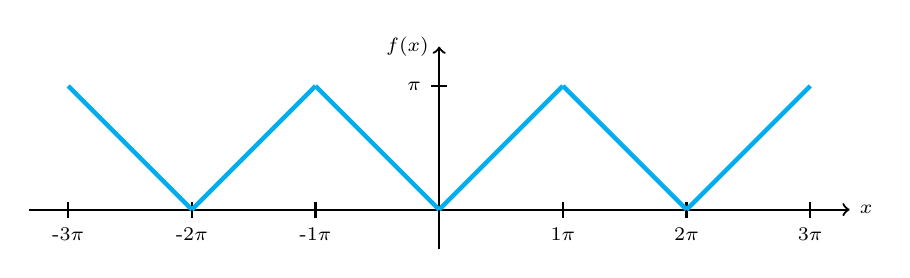
\begin{tikzpicture}[xscale=0.5,yscale=0.5]    				\begin{scope}[thick,font=\scriptsize]
					
					% Axes:
					% Are simply drawn using line with the `->` option to make them arrows:
					% The main labels of the axes can be places using `node`s:
					\draw [->] (-3.1415*3-1,0) -- (3.1415*3+1,0) node [right] {\(x\)};
					\draw [->]  (0,-1) -- (0,3.1415+1) node [left] {\(f(x)\)};
					
					% Axes labels:
					% Are drawn using small lines and labeled with `node`s. The placement can be set using options
					% Single
					% If you only want a single label per axis side:
					

					\draw (0.2,3.1415) -- (-0.2,3.1415) node [left] {\(\pi \)};
					
					\foreach \n in {-3,-2,-1,1,2,3}
					{
						\draw (3.1415*\n,0.2) -- (3.1415*\n, -0.2) node [below] { \n\(\pi \)};
					}
					
					\draw [cyan, ultra thick, domain= 0:3.1415] plot(\x,\x);
					\draw [cyan, ultra thick, domain= 0:3.1415] plot(-\x+2*3.1415,\x);
					\draw [cyan, ultra thick, domain= 0:3.1415] plot(\x+3.1415*2,\x);
					
					\draw [cyan, ultra thick, domain= 0:3.1415] plot(-\x,\x);
					\draw [cyan, ultra thick, domain= 0:3.1415] plot(\x-2*3.1415,\x);
					\draw [cyan, ultra thick, domain= 0:3.1415] plot(-\x-3.1415*2,\x);
					
					\end{scope}
					
					\end{tikzpicture}
					\caption{ \(f\) for intervallet \([-3\pi ,3\pi]\)}
				\end{figure}
			\end{enumerate}
			
			\item Siden \(f\) er \(\textbf{jevn}\): \(b_n=0\) 
			
			\begin{align*}
			a_0&=\frac{1}{L}\int\limits_{0}^{L}f(x)\, dx=\frac{1}{\pi}\int\limits_{0}^{\pi}f(x)\,dx\\&=\frac{1}{\pi}\int\limits_{0}^{\pi}x\,dx=\frac{\pi}{2}		
			\end{align*}
		    \begin{align*}
		    a_n&=\frac{2}{L}\int\limits_{0}^{L}f(x)\cos\frac{n\pi x}{L}\, dx = \frac{2}{\pi}\int\limits_{0}^{\pi}x\cos(nx)dx	\\
		    &= \frac{2}{\pi}\left[ \frac{\cos(nx)}{n^2}+\frac{x\sin(nx)}{n}	\right]_{0}^{\pi}=\frac{2}{n\pi}\left[ \cos(n\pi)-1 \right] \\
		    &=\frac{2}{n\pi}\left[ (-1)^n-1 \right]=\begin{cases}
		    0, \hspace{8pt} &\text{for n jevn}   \\
		    \frac{-4}{n\pi}, \hspace{8pt} &\text{for n odde}  
		    \end{cases}
		    \end{align*}
		    
		    \begin{align*}
		    Ff(x)&=a_0+\sum_{n=1}^{\infty}a_n\cos(nx)=\frac{\pi}{2}+\frac{2}{\pi}\sum_{n=1}^{\infty}\frac{1}{n^2}\left[ (-1)^n-1 \right]\cos(nx)\\
		    &=\frac{\pi}{2}+\frac{2}{\pi}\sum_{\text{n odde}}^{\infty}\frac{-2}{n^2}\cos(nx)=\underline{\underline{\frac{\pi}{2}-\frac{4}{\pi}\sum_{k=1}^{\infty}\frac{1}{(2k-1)^2}\cos((2k-1)x)}}
		    \end{align*}
		    
		    \item Ignorerer \(x=0\) 
		    
		    Ser at \[\frac{d}{dx}(f(x))=\frac{d}{dx}(|x|)=\begin{cases}
		    1, \hspace{16pt} &0<x<\pi\\
		    -1, \hspace{16pt} &-\pi<x<0
		    \end{cases}
		\]
	    og \[\frac{df}{dx}=g.\]
		
		Derfor 
		\begin{align*}
		Fg(x)&=\frac{d}{dx}\left[ Ff(x) \right]=\frac{d}{dx}\left[ \frac{\pi}{2}-\frac{4}{\pi}\sum_{k=1}^{\infty}\dfrac{1}{(2k-1)^2}\cos((2k-1)x) \right]\\
		&=\underline{\underline{\frac{4}{\pi}\sum_{k=1}^{\infty}\frac{1}{(2k-1)}\sin((2k-1)x )}}
		\end{align*}
		\item Tegner en skisse av \(g\)
		
		\begin{figure}[!ht]
			\centering
			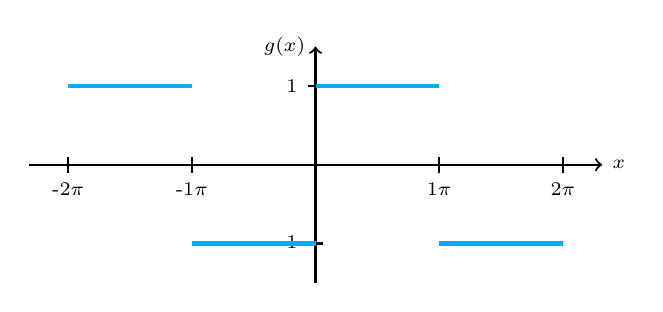
\begin{tikzpicture}[xscale=0.5,yscale=1]    				\begin{scope}[thick,font=\scriptsize]
			
			% Axes:
			% Are simply drawn using line with the `->` option to make them arrows:
			% The main labels of the axes can be places using `node`s:
			\draw [->] (-3.1415*2-1,0) -- (3.1415*2+1,0) node [right] {\(x\)};
			\draw [->]  (0,-1.5) -- (0,1.5) node [left] {\(g(x)\)};
			
			% Axes labels:
			% Are drawn using small lines and labeled with `node`s. The placement can be set using options
			% Single
			% If you only want a single label per axis side:
			
			
			\draw (0.2,1) -- (-0.2,1) node [left] {\(1\)};
			\draw (0.2,-1) -- (-0.2,-1) node [left] {\(-1\)};
			
			\foreach \n in {-2,-1,1,2}
			{
				\draw (3.1415*\n,0.2/2) -- (3.1415*\n, -0.2/2) node [below] { \n\(\pi \)};
			}
			
			\draw [cyan, ultra thick, domain= -2*3.1415:-3.1415] plot(\x,1);
			\draw [cyan, ultra thick, domain= -3.1415:0] plot(\x,-1);
			\draw [cyan, ultra thick, domain= 0:3.1415] plot(\x,1);
			\draw [cyan, ultra thick, domain= 3.1415:2*3.1415] plot(\x,-1);
			
			\end{scope}
			
			\end{tikzpicture}
			\caption{ skisse av \(g\)}
		\end{figure}
		
		nå,
		
		\[Fg(\pi)=\frac{1}{2}\left( g(\pi^+)+g(\pi^-)\right)= \frac{1}{2}(-1+1)=\underline{\underline{0}}. \]
		
		\item
		
		Finn en verdi av \(x\) for å sette inn i Fourier-rekken. Vi velger \(x=\frac{\pi}{2}\), siden vi da får et sinus uttrykk som kan forenkles. \(sin\left( (2k-1)\dfrac{\pi}{2}\right)=(-1)^{k+1} \)  
		
		\begin{align*}
		Fg\left( \frac{\pi}{2}\right) &=\frac{4}{\pi}\sum_{k=1}^{\infty}\frac{1}{(2k-1)}\sin\left( (2k-1)\frac{\pi}{2} \right) \\
		&=\frac{4}{\pi}\sum_{k=1}^{\infty}\frac{1}{(2k-1)}(-1)^{k+1}\\&=g\left( \frac{\pi}{2} \right) \hspace{32pt}\textit{av Fouriers teorem}\\
		&=1\\
		\frac{\pi}{4}&=\underline{\underline{\sum_{k=1}^{\infty}\dfrac{(-1)^{k+1}}{2k-1} =1-\frac{1}{3}+\frac{1}{5}-\frac{1}{7}+\cdots}}
		\end{align*}
		
		\end{enumerate}
		
		\newpage 
		
		\section{Deifferensligninger}
		
		\begin{fmindef}
		En ligning mellom forskjellige generelle ledd i en følge kalles en \textit{differensligning.} \medskip
		
		Dersom en differensligning involverer \(y_n,\,y_{n-1},\,\ldots,\, y_{n-d}, \) altså om den involverer \(d+1\) etterfølgende ledd i følgen, sier vi at ligningen er en differensligning av orden \(d\).\medskip
		
		En differensligning av orden \(d\) er lineær med konstante koeffisienter dersom den er på formen \[a_0y_n+a_1y_{n-1}+\ldots+a_dy_{n-d=f(n)} \]
		
		der høyre side er en funksjon av \(n\) (det vil si at \(f\) gir mening uten å tenke på følgen \(\left\lbrace y_n \right\rbrace \)). \medskip
		
		En lineær differensligning med konstante koeffisienter er i tillegg homogen dersom høyre side \(f\) er lik null. \medskip
		
		En differensligning av orden \(d\) trenger \(d\) startverdier for å bli entydig bestemt, vi må altså vite hva \(y_0,\,y_1,\,\ldots,\, y_{d-1} \) er for å få en tallfølge til svar.
		\end{fmindef}
		
		\subsection{Karakteristisk ligning og homogene differensligninger av andre orden}
		
		\begin{fmindef}
		La \[a_0y_n+a_1y_{n-1}+\ldots +a_dy_{n-d}=0 \]
		være en homogen lineær differensligning. Da kalles ligningen
		\[a_0\lambda^d+a_1\lambda^{d-1}+\ldots+a_{d-1}\lambda+a_d=0 \]
		\textit{den karakteristiske ligningen} til differensligningen.
		\end{fmindef}
		
		\begin{fteo}
		Den geometriske følgen \(y_n=\lambda^n \) er en løsning til en homogen lineær differensliging med konstante koeffisienter hvis og bare hvis \(\lambda \) er en rot i den karakteristiske ligningen.
		\end{fteo}
		
		\begin{fteo}
		Den generelle løsningen til en homogen lineær differensligning av andre orden, med konstante koeffisienter, avhenger av røttene til den karakteristiske ligningen og er gitt slik:
		
		\begin{enumerate}
			\item Dersom det er to ulike reelle røtter \(\lambda_1 \) og \(\lambda_2 \), er den generelle løsningen \[y_n=A\cdot \lambda_{1}^{n}+B\cdot\lambda_{2}^{n}. \]
			\item Dersom det er en dobbel reell rot \(\lambda \), er den generelle løsningen 
			\[y_n = (A+B_n)\cdot \lambda^n. \]
			\item Dersom det er komplekse løsninger \(\lambda = re^{\pm i\theta} \), er den generelle løsningen \[y_n=r^n(A\cos{n\theta}+B\sin{n\theta}). \]
		\end{enumerate}
		\end{fteo}
		
		\newpage
		
		\subsection{Inhomogene differensligninger}
		
		En lineær differensligning på formen \[a_0y_n+a_1y_{n-1}+\ldots + a_dy_{n-d}=f(n) \]
		kalles \textit{inhomogen} forutsatt at \(f(n)\neq 0. \) Å finne den generelle løsningen til slike differensligninger er en utregning i to separate steg:
		
		\begin{itemize}
			\item Vi bruker karakteristisk ligning for å finne den generelle løsningen til den tilhørende homogene differensligningen. Vi bruker notasjonen \(y_n^{(h)} \) for denne følgen.
			\item Vi trenger en partikulær løsning til den inhomogene differensligningen. Den finner vi gjerne ved ubestemte koeffisienters metode. Vi bruker notasjonen \(y_n^{(p)} \) for en slik partikulær løsning. 
		\end{itemize}
		Den generelle løsningen til den inhomogene differensligningen er nå gitt ved \[y_n=y_n^{(h)}+y_n^{(p)}. \]
		Dersom det er oppgitt tilstrekkelig mange startverdier, utfører vi følgende steg til slutt:
		
		\begin{itemize}
			\item Vi bestemmer konstantene i den generelle løsningen ved å stille opp ligningsystemet gitt ved startverdiene.
		\end{itemize}
		
		Å løse den tilsvarende homogene differensligningen har vi allerede lært. Neste steg er å lete etter en partikulær løsning. Vi skal med utgangspunkt i uttrykket \(f(n)\) tippe formen på \(y_n^{(p)}\) og deretter bestemme koeffisienter ved regning. Dette kalles ofte \textit{ubestemte koeffisienters metode}. Siden løsningen til den homogene ligningen kan påvirke hvordan vi tipper formen på partikulær løsning, er det viktig å gjøre stegene i riktig rekkefølge. 
		
		Vi setter opp en tabell som indikerer hvordan formen på partikulær løsning bør tippes:
		
		\def\arraystretch{2.5}%
		\begin{table}[!ht]
			\centering
			\label{my-label}
			\begin{tabular}{c c}
				
				\underline{\(f(n)\) } &  \underline{\(y_n^{(p)}\)}                          \\ \hline
				\(c\)       & \(M\)                         \\ \hline
				\(an+b \)          & \(Mn+N\)                              \\ \hline
				\(an+bn+c \)          & \(Mn^2+Nn+P\)                                 \\ \hline
				\(a_rn^r+\ldots + a_1n+a_0 \)   & \(M_rn^r+\ldots + M_1n+M_0\)                                \\ \hline
				\(ak^n \)   & \(Mk^n\)                                \\ \hline
				\((an+b)k^n \)   & \((Mn+N)k^n \)                                \\ \hline
				\((a_rn^r+\ldots + a_1n+a_0)k^n \)   & \((M_rn^r+\ldots + M_1n+M_0)k^n\)  \\ \hline
				\(a\cos{n\phi} \)          & \(M\cos{n\phi}+N\sin{n\phi} \)          \\ \hline
				\(a\sin{n\phi} \)        &        \(M\cos{n\phi}+N\sin{n\phi} \)          \\ \hline
				\(ak^n\cos{n\phi} \)   & \((M\cos{n\phi}+N\sin{n\phi})k^n \)                     \\ \hline
				\(ak^n\sin{n\phi} \)  & \((M\cos{n\phi}+N\sin{n\phi})k^n \)   \\ \hline
			\end{tabular}
		\end{table}
		
		\def\arraystretch{1}%
		\newpage
		
		Det finnes untakstilfeller:
		
		\textbf{Å øke graden}
		
		Dersom ledd i \(f(n)\) passer inn i løsningen til den homogene \(y_n^{(h)}\), multipliserer vi uttrykkene for \(y_n^{(p)} \) i tabellen ovenfor med \(n\). Gjenta om nødvendig.
		
		\textbf{Superposisjon}
		
	    Hvis \(f(n)\) er summen av flere typer ledd. danner vi formen på \(y_n^{(p)}\), ved å summere de tilsvarende forslagene gitt i tabellen. Husk å endre navn på de ubestemte koeffisientene etter hvert ledd. 
        
         		
		\newpage
		\begin{center}
			%Flowchart
			\scalebox{0.9}{
				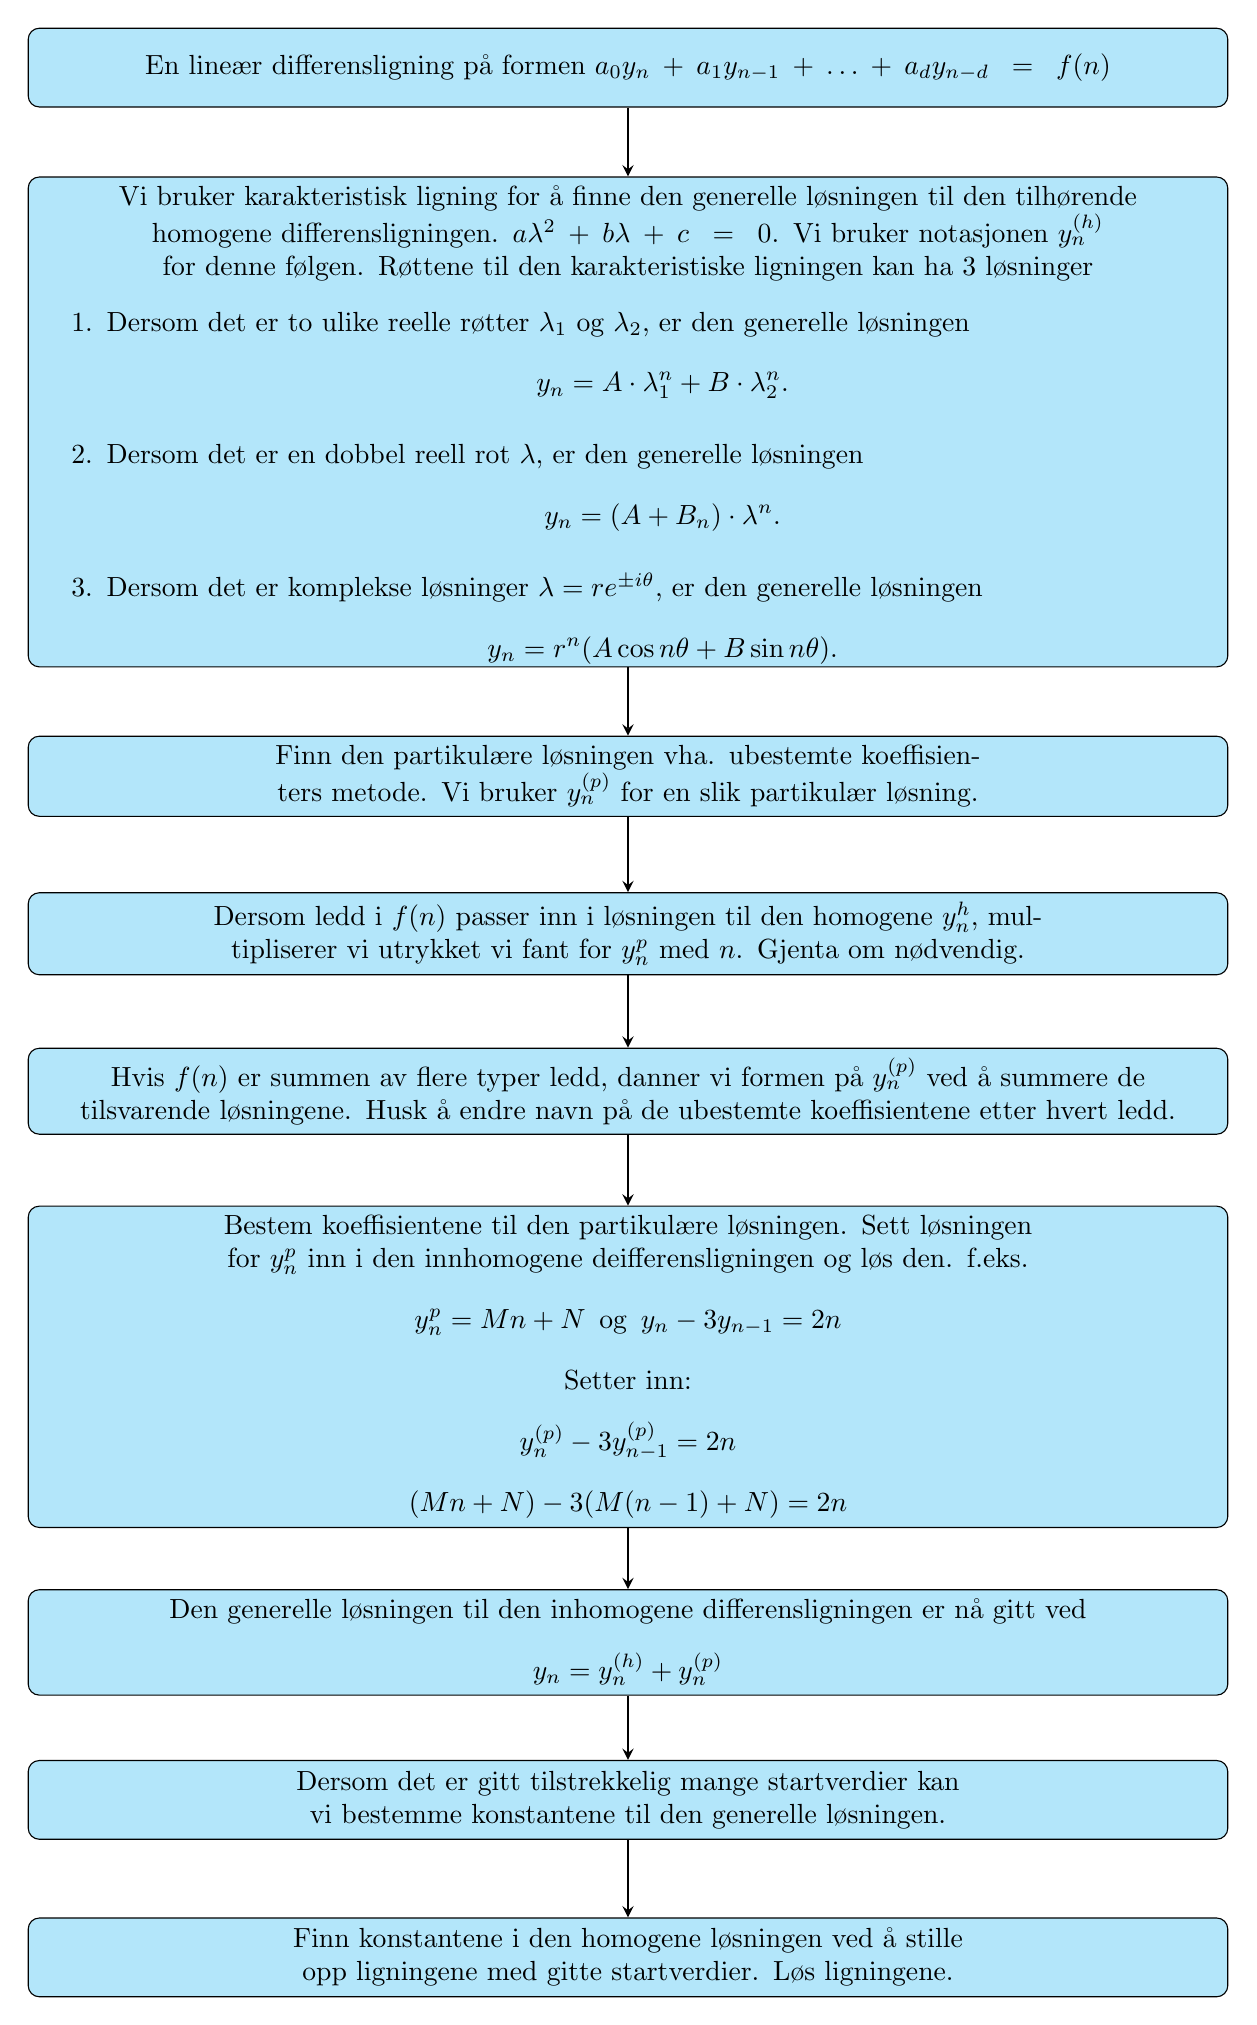
\begin{tikzpicture}[node distance=2cm, auto]
				\centering
				
				\node (steg1) [prosess, text width=15cm] {En lineær differensligning på formen \(a_0y_n+a_1y_{n-1}+\ldots+a_dy_{n-d}=f(n) \)};
				
				\begin{scope}[node distance=4.5cm]
				
				\node (steg2) [prosess, below of=steg1, text width=15cm] {Vi bruker karakteristisk ligning for å finne den generelle løsningen til den tilhørende homogene differensligningen. \(a\lambda^2+b\lambda+c=0 \). Vi bruker notasjonen \(y_n^{(h)}\) for denne følgen. Røttene til den karakteristiske ligningen kan ha 3 løsninger \begin{enumerate}
					\item Dersom det er to ulike reelle røtter \(\lambda_1 \) og \(\lambda_2 \), er den generelle løsningen \[y_n=A\cdot \lambda_{1}^{n}+B\cdot\lambda_{2}^{n}. \]
					\item Dersom det er en dobbel reell rot \(\lambda \), er den generelle løsningen 
					\[y_n = (A+B_n)\cdot \lambda^n. \]
					\item Dersom det er komplekse løsninger \(\lambda = re^{\pm i\theta} \), er den generelle løsningen \[y_n=r^n(A\cos{n\theta}+B\sin{n\theta}). \]
					\end{enumerate}
					};
				\node (steg3) [prosess,below of=steg2, text width=15cm] {Finn den partikulære løsningen vha. ubestemte koeffisienters metode. Vi bruker \(y_n^{(p)}\) for en slik partikulær løsning.};
				\end{scope}
				\node (steg4) [prosess,below of=steg3, text width=15cm] {Dersom ledd i \(f(n)\) passer inn i løsningen til den homogene \(y_n^{h}\), multipliserer vi utrykket vi fant for \(y_n^{p}\) med \(n\). Gjenta om nødvendig.};
				\node (steg5) [prosess,below of=steg4, text width=15cm] {Hvis \(f(n)\) er summen av flere typer ledd, danner vi formen på \(y_n^{(p)}\) ved å summere de tilsvarende løsningene. Husk å endre navn på de ubestemte koeffisientene etter hvert ledd.};
				
				\begin{scope}[node distance=3.5cm]
				\node (steg6) [prosess,below of=steg5, text width=15cm] {Bestem koeffisientene til den partikulære løsningen. Sett løsningen for \(y_n^{p}\) inn i den innhomogene deifferensligningen og løs den. f.eks.
					\[y_n^{p}=Mn+N\,\,\,  \text{og} \,\,\,y_n-3y_{n-1}=2n\]
					Setter inn:
					\[y_n^{(p)}-3y_{n-1}^{(p)}=2n\]
					\[(Mn+N)-3(M(n-1)+N)=2n\]
				};
				
				\node (steg7) [prosess,below of=steg6, text width=15cm] {Den generelle løsningen til den inhomogene differensligningen er nå gitt ved \[y_n=y_n^{(h)}+y_n^{(p)}\] };
				\end{scope}
				\node (steg8) [prosess,below of=steg7, text width=15cm] {Dersom det er gitt tilstrekkelig mange startverdier kan vi bestemme konstantene til den generelle løsningen.};
				\node (steg9) [prosess,below of=steg8, text width=15cm] {Finn konstantene i den homogene løsningen ved å stille opp ligningene med gitte startverdier. Løs ligningene.};
				

				
				\draw [arrow] (steg1) -- (steg2);
				\draw [arrow] (steg2) -- (steg3);
				\draw [arrow] (steg3) -- (steg4);
				\draw [arrow] (steg4) -- (steg5);
				\draw [arrow] (steg5) -- (steg6);
				\draw [arrow] (steg6) -- (steg7);
				\draw [arrow] (steg7) -- (steg8);
				\draw [arrow] (steg8) -- (steg9);
				
				\end{tikzpicture}
			}
		\end{center}
		\newpage
		
		
		\newpage
		
		\section{Lineær algebra}
		
		\subsection{Trappeform}
		
		\begin{fmindef}
			I en rad kaller vi det første elementet som er forskjellig fra null, for det \textit{ledende elementet}. En matrise er på \textit{trappeform} dersom 
			\begin{enumerate}
				\item Hver rad har en 1-er som ledende element eller består bare av nuller.
				\item Eventuelle rader bestående bare av nuller er nederst i matrisen.
				\item Hver blokk av matrsien som har en ledende 1-er i øverste høyre hjørne, består ellers bare av nuller.
			\end{enumerate}
		\end{fmindef}
		
		\subsection{Redusert trappeform}
		
		\begin{fmindef}
			En matrise er på \textit{redusert trappeform} dersom
			
			\begin{enumerate}
				\item Hver rad har en 1-er som ledende element eller består bare av nuller.
				\item Eventuelle rader bestående bare av nuller er nederst i matrisen.
				\item Hver blokk av matrsien som har en ledende 1-er i øverste høyre hjørne, består ellers bare av nuller.
				\item Hver kolonne i matrisen som inneholder en ledende 1-er, består ellers bare av nuller.
			\end{enumerate}
		\end{fmindef}
		
		\newpage
		
		\subsection{Determinanter}
		
		\subsubsection{2x2 matrise}
		
		\begin{fmindef}
			Dterminten til en 2x2 matrise er
			
			\[det \left[ 	\begin{array}{rr} 
			a & b   \\
			c & d
			\end{array} \right]
			= \left| \begin{array}{rr} 
			a & b \\
			c & d
			\end{array} \right|=ad-bc \]
		\end{fmindef}
		
		\subsubsection{3x3 matrise}
		
		\begin{mindef}
			Metode for å finne detrminanter i 3x3 matriser
			
			
			
			\[A=\left[\begin{array}{rrr} 
			a_{11} & a_{12} & a_{13} \\
			a_{21} & a_{22} & a_{23} \\
			a_{31} & a_{32} & a_{33}
			\end{array} \right], \hspace{16pt} \left[\begin{array}{rrr} 
			+ & - & + \\
			- & + & - \\
			+ & - & +
			\end{array} \right] \]
			
			For å finne determinanten må du velge en rekke eller en kolonne du vil bruke. Oftest lurt å ta den med flest nuller.
			
			Eks. Velger øverste rad
			
			\[A=\left[\begin{array}{ccc} 
			\MyTikzmark{leftA}{a_{11}}& a_{12} & \MyTikzmark{rightA}{a_{13}} \\
			a_{21} & a_{22} & a_{23} \\
			a_{31} & a_{32} & a_{33}
			\end{array} \right], \hspace{16pt}\left[\begin{array}{rrr} 
			+ & - & + \\
			- & + & - \\
			+ & - & +
			\end{array} \right]\]
			\(\DrawHLine[cyan, line width=4mm, opacity=0.3]{leftA}{rightA}\)
			
			\[\left[\begin{array}{rrr} 
			+\textcolor{red}{\textbf{a}_{\textbf{11}}} & \textcolor{gray}{a_{12}} & \textcolor{gray}{a_{13}} \\
			\textcolor{gray}{a_{21}} & \textbf{a}_{\textbf{22}} & \textbf{a}_{\textbf{23}} \\
			\textcolor{gray}{a_{31}} & \textbf{a}_{\textbf{32}} & \textbf{a}_{\textbf{33}}
			\end{array} \right],\hspace{16pt}\left[\begin{array}{rrr} 
			\textcolor{gray}{a_{11}} & -\textcolor{red}{\textbf{a}_{\textbf{12}}} & \textcolor{gray}{a_{13}} \\
			\textbf{a}_{\textbf{21}} & \textcolor{gray}{a_22} & \textbf{a}_{\textbf{23}} \\
			\textbf{a}_{\textbf{31}} & \textcolor{gray}{a_{32}} & \textbf{a}_{\textbf{33}}
			\end{array} \right]
			,\hspace{16pt}\left[\begin{array}{rrr} 
			\textcolor{gray}{a_{11}} & \textcolor{gray}{a_{12}} & +\textcolor{red}{\textbf{a}_{\textbf{13}}} \\
			\textbf{a}_{\textbf{21}} & \textbf{a}_{\textbf{22}} & \textcolor{gray}{{a}_{23}} \\
			\textbf{a}_{\textbf{31}} & \textbf{a}_{\textbf{32}} & \textcolor{gray}{a_{33}}
			\end{array} \right]\]
			
			Da er determinanten til \(A\)
			
			\[det\,A=\left|\begin{array}{rrr} 
			a_{11} & a_{12} & a_{13} \\
			a_{21} & a_{22} & a_{23} \\
			a_{31} & a_{32} & a_{33}
			\end{array} \right|=a_{11}\left|\begin{array}{rr} 
			a_{22} & a_{23}  \\
			a_{32} & a_{33} 
			\end{array} \right| - a_{12}\left|\begin{array}{rr} 
			a_{21} & a_{23} \\
			a_{31} & a_{33}
			\end{array} \right|+a_{13}\left|\begin{array}{rr} 
			a_{21} & a_{22} \\
			a_{31} & a_{32}
			\end{array} \right|
			\]
		
				        
        Det går an å velge både rekker og kolonner når du skal finne determinanaten. 
        
        Her er et eksempel der vi velger den midterste kolonnen
        
        \[A=\left[\begin{array}{ccc} 
        a_{11}& \MyTikzmark{A}{a_{12}} & a_{13} \\
        a_{21} & a_{22} & a_{23} \\
        a_{31} & \MyTikzmark{B}{a_{32}} & a_{33}
        \end{array} \right], \hspace{16pt}\left[\begin{array}{rrr} 
        + & - & + \\
        - & + & - \\
        + & - & +
        \end{array} \right]\]
        \(\DrawVLine[cyan, line width=6mm, opacity=0.3]{A}{B}\)
		
		\[\left[\begin{array}{rrr} 
		\textcolor{gray}{a_{11}} & -\textcolor{red}{\textbf{a}_{\textbf{12}}} & \textcolor{gray}{a_{13}} \\
		\textbf{a}_{\textbf{21}} & \textcolor{gray}{a_22} & \textbf{a}_{\textbf{23}} \\
		\textbf{a}_{\textbf{31}} & \textcolor{gray}{a_{32}} & \textbf{a}_{\textbf{33}}
		\end{array} \right]
		,\hspace{16pt}\left[\begin{array}{rrr} 
		\textbf{a}_{\textbf{11}} & \textcolor{gray}{a_{12}} & \textbf{a}_{\textbf{13}} \\
		\textcolor{gray}{a_{21}} & +\textcolor{red}{\textbf{a}_\textbf{22}} & \textcolor{gray}{a_{23}} \\
		\textbf{a}_{\textbf{31}} & \textcolor{gray}{a_{32}} & \textbf{a}_{\textbf{33}}
		\end{array} \right]
		,\hspace{16pt}\left[\begin{array}{rrr} 
		\textbf{a}_{\textbf{11}} & \textcolor{gray}{a_{12}} & \textbf{a}_{\textbf{13}} \\
		\textbf{a}_{\textbf{21}} & \textcolor{gray}{a_{22}} & \textbf{a}_{\textbf{23}} \\
		\textcolor{gray}{a_{31}} & -\textcolor{red}{\textbf{a}_\textbf{{32}}} & \textcolor{gray}{a_{33}}
		\end{array} \right]\]
		
		Da er determinanten til \(A\)
		
		\[det\,A=\left|\begin{array}{rrr} 
		a_{11} & a_{12} & a_{13} \\
		a_{21} & a_{22} & a_{23} \\
		a_{31} & a_{32} & a_{33}
		\end{array} \right|=-a_{12}\left|\begin{array}{rr} 
		a_{21} & a_{23}  \\
		a_{31} & a_{33} 
		\end{array} \right| + a_{22}\left|\begin{array}{rr} 
		a_{11} & a_{13} \\
		a_{31} & a_{33}
		\end{array} \right|-a_{32}\left|\begin{array}{rr} 
		a_{11} & a_{13} \\
		a_{21} & a_{23}
		\end{array} \right|
		\]
		\end{mindef}
		
		\newpage
		
		\subsection{Singulær matrise}
		
		\begin{fmindef}
			Hvis determinaneten til en kvadratisk matrise A er ulik null, har matrisen en invers.
			
			\[det\,A \neq 0 \rightarrow \text{matrisen har en invers} \]
			
			Hvis determinanten til matrisen A er lik null er matrisen singulær. Har ingen invers.
			
			\[det\,A = 0 \rightarrow \text{matrisen er singulær} \]
			
		\end{fmindef}
		
		\newpage
		
		\subsection{Inverse matriser}
		
		\begin{fminset}
			Kofaktor matrisen til en 2x2 matrise
			
			\[A= \left[\begin{array}{rr} 
			a & b \\
			c & d
			\end{array} \right] \]
			
		    For å finne kofakotrene til \(A\) må vi finne minorene til til matrisen. Hvis minorene ligger i et pluss minus felt er de lik kofakotorene.
		    
		    \[C= \left[\begin{array}{rr} 
		    +M_{11} & -M_{12} \\
		    -M_{21} & +M_{22}
		    \end{array} \right] =
		    \left[\begin{array}{rr} 
		    C_{11} & C_{12} \\
		    C_{21} & C_{22}
		    \end{array} \right] \]
		    
		    \[M_{11}=\left[\begin{array}{rr} 
		    \textcolor{gray}{a} & \textcolor{gray}{b} \\
		    \textcolor{gray}{c} & \textbf{d} 
		    \end{array} \right]=d, \hspace{16pt}
		    M_{12}=\left[\begin{array}{rr} 
		    \textcolor{gray}{a} & \textcolor{gray}{b} \\
		    \textbf{c} & \textcolor{gray}{d} 
		    \end{array} \right]=c \]
		    \[M_{21}=\left[\begin{array}{rr} 
		    \textcolor{gray}{a} & \textbf{b} \\
		    \textcolor{gray}{c} & \textcolor{gray}{d} 
		    \end{array} \right]=b, \hspace{16pt}
		    M_{22}=\left[\begin{array}{rr} 
		    \textbf{a} & \textcolor{gray}{b} \\
		    \textcolor{gray}{c} & \textcolor{gray}{d}
		    \end{array} \right]=a \]
			
			Kofaktormatrisen til \(A\) blir derfor
			
			\[C=\left[\begin{array}{rr} 
			+M_{11} & -M_{12} \\
			-M_{21} & +M_{22}
			\end{array} \right]=\left[\begin{array}{rr} 
			d & -c \\
			-b & a
			\end{array} \right]\]
		\end{fminset}
		
		\begin{fmindef}
			Den \textit{adjungerte} matrisen til en kvadratisk matrise \(A\) er den transponerte av kofaktormatrisen.
			\[\text{adj}\,A=C^{T} \]
		\end{fmindef}
		
		\begin{fteo}
			En kvadratisk matrise \(A\) er invertibel hvis og bare hvis \(A\neq 0\). 
			I så fall er den inverse matrisen gitt ved formelen
			
			\[A^{-1}=\frac{1}{\text{det}\, A}\,\text{adj}\,A \].
			
		\end{fteo}		
		
		\subsubsection{Invers til 2x2 matrisen}
	    
	    \[A=\left[\begin{array}{rr} 
	    a & b \\
	    c & d
	    \end{array} \right]\]
		
		\[det\,A=ad-bc, \hspace{16pt} adj\, A= C^T=\left[\begin{array}{rr} 
		d & -c \\
		-b & a
		\end{array} \right]^T=\left[\begin{array}{rr} 
		d & -b \\
		-c & a
		\end{array} \right] \]
		
		\[A^{-1}=\frac{1}{\text{det}\, A}\,\text{adj}\,A=\frac{1}{ab-bc}\left[\begin{array}{rr} 
		d & -b \\
		-c & a
		\end{array} \right] \]
		
		\newpage
		
		\subsubsection{Invers til 3x3 matrisen}
		
		\begin{fminset}
			Kofaktor matrisen til en 3x3 matrise
			
			\[A=\left[\begin{array}{rrr} 
			a_{11} & a_{12} & a_{13} \\
			a_{21} & a_{22} & a_{23} \\
			a_{31} & a_{32} & a_{33}
			\end{array} \right]
			\]
			
			For å finne kofakotrene til \(A\) må vi finne minorene til til matrisen. Hvis minorene ligger i et pluss minus felt er de lik kofakotorene.
			
			\begin{align*}
			C=\left[\begin{array}{rrr} 
			+M_{11} & -M_{12} & +M_{13} \\
			-M_{21} & +M_{22} & -M_{23} \\
			+M_{31} & -M_{32} & +M_{33}
			\end{array} \right]&=
			\left[\begin{array}{ccc} 
			+\Big| \begin{array}{cc}
			a_{22} & a_{23} \\ a_{32} & a_{33}
			\end{array}\Big|  & -\Big| \begin{array}{cc}
			a_{21} & a_{23} \\ a_{31} & a_{33}
			\end{array}\Big| & +\Big| \begin{array}{cc}
			a_{21} & a_{22} \\ a_{31} & a_{32}
			\end{array}\Big| \\
			-\Big| \begin{array}{cc}
			a_{12} & a_{13} \\ a_{32} & a_{33}
			\end{array}\Big| & +\Big| \begin{array}{cc}
			a_{11} & a_{13} \\ a_{31} & a_{33}
			\end{array}\Big| & -\Big| \begin{array}{cc}
			a_{11} & a_{12} \\ a_{31} & a_{32}
			\end{array}\Big| \\
			+\Big| \begin{array}{cc}
			a_{12} & a_{13} \\ a_{22} & a_{23}
			\end{array}\Big| & -\Big| \begin{array}{cc}
			a_{11} & a_{13} \\ a_{21} & a_{23}
			\end{array}\Big| & +\Big| \begin{array}{cc}
			a_{11} & a_{12} \\ a_{21} & a_{22}
			\end{array}\Big|
			\end{array} \right] \\ &=
			\left[\begin{array}{rrr} 
			C_{11} & C_{12} & C_{13} \\
			C_{21} & C_{22} & C_{23}  \\
			C_{31} & C_{32} & C_{33}
			\end{array} \right]
			\end{align*}
			
		\end{fminset}
		
		\begin{fminset} Invers til 3x3 matrisen
			
		\[A=\left[\begin{array}{rrr} 
		a_{11} & a_{12} & a_{13} \\
		a_{21} & a_{22} & a_{23} \\
		a_{31} & a_{32} & a_{33}
		\end{array} \right]
		\]
		
		\[det\,A=\left|\begin{array}{rrr} 
		a_{11} & a_{12} & a_{13} \\
		a_{21} & a_{22} & a_{23} \\
		a_{31} & a_{32} & a_{33}
		\end{array} \right|=a_{11}\left|\begin{array}{rr} 
		a_{22} & a_{23}  \\
		a_{32} & a_{33} 
		\end{array} \right| - a_{12}\left|\begin{array}{rr} 
		a_{21} & a_{23} \\
		a_{31} & a_{33}
		\end{array} \right|+a_{13}\left|\begin{array}{rr} 
		a_{21} & a_{22} \\
		a_{31} & a_{32}
		\end{array} \right|\]
		
		
		\[\text{adj}\,A=C^T= \left[\begin{array}{rrr} 
		C_{11} & C_{12} & C_{13} \\
		C_{21} & C_{22} & C_{23}  \\
		C_{31} & C_{32} & C_{33}
		\end{array} \right]^T=\left[\begin{array}{rrr} 
		C_{11} & C_{21} & C_{31} \\
		C_{12} & C_{22} & C_{32}  \\
		C_{13} & C_{23} & C_{33}
		\end{array} \right] \]
		
	    \[A^{-1}=\frac{1}{\text{det}\, A}\,\text{adj}\,A \]
		\end{fminset}
		
		\newpage
		
		\subsection{Pivot-element}
		
		\begin{fmindef}
			Det første elementet i hver rekke som ikke er lik null i en matrise som er på trappeform er et pivot element. Den kolonnen med pivot-elementet blir kalt en pivot-kolonne.
		\end{fmindef}
		
		\begin{mitteks}
			\[
			\left[\begin{array}{lllll} 
				3^* & 0 & 2 & 7 & 5\\
				0 & 0 & 1^* & 0 & 8\\
				0 & 0 & 0 & 0 & 7^* \\
				0 & 0 & 0 & 0 & 0 \\
				0 & 0 & 0 & 0 & 0 
			\end{array} \right]\]
		\end{mitteks}
		
		\subsection{Rang}
		
		\begin{fmindef}
			Antall pivot-elementer i en matrise som er gjennomgått Gauss-eliminasjon. Rangen til en matrise A skrives: rang A.
			\[\text{rang}(A^T)=\text{rang(A)} \]
		\end{fmindef}
		
		\begin{mitteks}
			
		Finn rangen til matrise A
		
		\[A=\left[\begin{array}{rrr} 
		3 & 1 & 2 \\
		0 & 0 & 1 \\
		1 & 1 & -1
		\end{array} \right]\]	
		
		\begin{align*}
		\underset{\sim}{R_2\leftrightarrow R_3} 
		\left[\begin{array}{rrr} 
		3 & 1 & 2 \\
		1 & 1 & -1 \\
		0 & 0 & 1
		\end{array} \right]\hspace{16pt}\underset{\sim}{R_1\leftrightarrow R_2}\left[\begin{array}{rrr} 
		1 & 1 & -1 \\
		3 & 1 & 2 \\
		0 & 0 & 1
		\end{array} \right] \hspace{16pt}
		\underset{\sim}{R_2=R_2-3R_1}
		\left[\begin{array}{lcr} 
		1^* & 1 & -1 \\
		0 & -2^* & 5 \\
		0 & 0 & 1^*
		\end{array} \right] 
		\end{align*}
		
		\[\underline{\underline{\text{rang A}=3}}\]
		\end{mitteks}
		
		\subsection{Relaterte begreper}
		
		\begin{fteo}
			La \(A\) være en kvadratisk matrise. Følgende påstander er ekvivalente:
			
			\begin{enumerate}
				\item Ligningsystemer \(A\vec{x}=\vec{b} \) med \(A\) som koeffisientmatrise, har nøyaktig en løsning.
				\item Kolonnene i \(A\) er lineært uavhengige vektorer.
				\item Ligningsystemet \(A\vec{x}=\vec{0} \) har nøyaktig en løsning.
				\item Matrisen \(A\) er radekvivalent til identitetsmatrisen \(I\).
				\item Matrisen \(A\) er invertibel.
				\item det \(A\neq 0 \).
			\end{enumerate}
		\end{fteo}
		
		
		\newpage
		
		\subsection{Egenverdier og egenvektorer}
		
		\begin{fmindef}
		La \(A\) være en kvadratisk matrise. En vektor \(\vec{v}\in \mathbb{R}^n\) kalles en egenvektor for \(A\) dersom \(\vec{v}\neq \vec{0} \) og \(A\vec{v}\) er parallell med \(\vec{v} \):
		\[A\vec{v}=\lambda\vec{v} \]
		Tallet \(\lambda \) kalles \textit{egenverdien} for \(A\) tilhørende \(\vec{v} \).
		\end{fmindef}
		
		\begin{fmitteks}
		La \(2\times 2 \)-matrisen \(A\) være gitt som 
		\[A=\left[\begin{array}{rr} 
		3 & 1 \\
		4 & 0
		\end{array} \right]\]
		Om vi betrakter den tilhørende lineære transformasjonen fra planet på seg selv, kan vi se hva som skjer
		med følgende vektorer:
		\[\vec{u}=\left[\begin{array}{rr} 
		0 \\
		1
		\end{array} \right]
		,\hspace{16pt}
		\vec{v}=\left[\begin{array}{rr} 
		1 \\
		1
		\end{array} \right]
		,\hspace{16pt}
		\vec{w}=\left[\begin{array}{rr} 
		1 \\
		0
		\end{array} \right]
		 \]
		Matrisemultiplikasjon gir
		\[A\vec{u}=\left[\begin{array}{rr} 
		1 \\
		0
		\end{array} \right]
		,\hspace{16pt}
		A\vec{v}=\left[\begin{array}{rr} 
		4 \\
		4
		\end{array} \right]
		,\hspace{16pt}
		A\vec{w}=\left[\begin{array}{rr} 
		3 \\
		4
		\end{array} \right].
		\]
		Vi ser at verken \(\vec{u}\) eller \(\vec{w} \) er en egenvektoer, men
		
		\[
		\vec{v}=\left[\begin{array}{rr} 
		1 \\
		1
		\end{array} \right]  \text{ er egenvektor for } A \text{ med egenverdi } \lambda=4.\]
		\end{fmitteks}
		
		\begin{fteo}
			L \(A\) være en \(n\,x\,n \)-matrise. Egenverdien til \(A\) er løsningen på ligningen
			\[det(A-\lambda I)=0\]
			For hver løsning \(\lambda_{i}\) til denne ligningen finnes de tilhørende
			egenvektorene som løsninger til ligningssystemet
			\[(A-\lambda_iI)\cdot \vec{v}=\vec{0} \] 
		\end{fteo}
		
		
		\newpage
		
		\subsection{Nullrommet}
		
		\begin{fmindef}
		Finn en basis for nullrommet til A.
		
		 Basis for nullrommet til en matrise er mengden av alle x-vektorer som løser denne ligningen.
		
		\[A\vec{x}=\vec{0} \]
		
		Vi kan bytte ut A med A på redusert trappeform.
		
		\[\text{rref}(A)\vec{x}=\vec{0} \] 
		
		rref = Reduced Row-Echelon Form = redusert trappeform.
		\end{fmindef}
		
		\begin{mitteks}
		Finn en basis for nullrommet til A
		\[A=\left[\begin{array}{rrrr} 
		1 & -2 & -1 & -1 \\
		1 & -2 & 0 & 1 \\
		-2 & 4 & 1 & 0 
		\end{array} \right]\]
		
		Begynner med å finne matrise A på redusert trappeform. Hopper over utregningen.
		
		\[\text{rref}(A)=\left[\begin{array}{rrrr} 
		1^{*} & -2 & 0 & 1 \\
		0 & 0 & 1^{*} & 2 \\
		0 & 0 & 0 & 0 
		\end{array} \right]\]
		
	    Vi setter opp ligningen: \(\text{rref}(A)\vec{x}=\vec{0}\)
		
		\[\left[\begin{array}{rrrr} 
		1 & -2 & 0 & 0 \\
		0 & 0 & 1 & 2 \\
		0 & 0 & 0 & 0 
		\end{array} \right] \left[\begin{array}{c} 
		x_1  \\
		x_2  \\
		x_3  \\
		x_4
		\end{array} \right]=
		\left[\begin{array}{rr} 
		0  \\
		0  \\
		0
		\end{array} \right] \]
		
		Vi ser at det kun er søyle \(x_1\) og søyle \(x_3\) som har pivot-elementer og er pivot-søyler. Derfor er \(x_2\) og \(x_4\) frie variabler. Vi setter de lik parameterene s og t.
		
		\[x_2=s,\hspace{16pt} x_4=t \]
		
		Ganger ut ligningen og setter inn for \(x_2\) og \(x_4\)
		
		\begin{align*}
		x_1-2x_2+x_4=0\hspace{8pt}&\Rightarrow \hspace{8pt}x_1=2s-t\\
		x_3+2x_4=0\hspace{8pt}&\Rightarrow\hspace{8pt} x_3=-2t
		\end{align*}
		
		Setter opp x-vektoren
		
		\[\left[\begin{array}{c} 
		x_1 \\
		x_2 \\
		x_3 \\
		x_4
		\end{array} \right]=\left[\begin{array}{c} 
		2s-t\\
		s   \\
		-2t \\
		t
		\end{array} \right]=s\left[\begin{array}{c} 
		2 \\
		1 \\
		0 \\
		0
		\end{array}\right]+t\left[\begin{array}{r} 
		-1 \\
		0  \\
		-2 \\
		1		\end{array}  \right] \]
		Vi har nå funnet de to vektorene som utgjør basisen til nullrommet. Nullrommet til vektor A:
		\[N(A)=\left\lbrace\left[\begin{array}{c} 
		2 \\
		1 \\
		0 \\
		0
		\end{array}\right],\left[\begin{array}{r} 
		-1 \\
		0  \\
		-2 \\
		1		\end{array}  \right] \right\rbrace \]
		
		\end{mitteks}
		
		\newpage
		
		\subsection{Diagonalisering}
		
		\begin{fteo}
			La \(A\) være en \(n\times n \)-matrise, og anta at den har \(n\) lineært uavhengige egenvektorer \(\vec{v}_1,\vec{v}_2,\cdots,\vec{v}_n \). La \(P\) være matrisen med de valgte egenvektorene som kolonner:
			\[P=\left(\vec{v}_1|\vec{v}_2|\cdots|\vec{v}_n \right) \]
			Da er \(P\) inverterbar, og
			\[A=PDP^{-1}\]
			der \(D\) er diagonalmatrisen
			\[D=\left[\begin{array}{cccc} 
			\lambda_1 & 0 & \cdots & 0 \\
			0 & \lambda_2 & \cdots & 0 \\
			\vdots & \vdots & \ddots & \vdots \\
			0 & 0 & \cdots & \lambda_n
			\end{array} \right]\]
			Elementene langs diagonalen er egenveridene \(\lambda_i \), som svarer til egenvektorene \(\vec{v}_i \).
		\end{fteo}
		
		\begin{fmindef}
			En \(n\times n \)-matrise \(A\) kalles \textit{diagonaliserbar} dersom den kan skrives på formen \[A=PDP^{-1}\]
			for en diagonal matrise \(D\) og en inverterbar matrise \(P\).
			
			Kan også omskrives 
			
			\[A=PDP^{-1} \Longleftrightarrow AP=PD \Longleftrightarrow D=P^{-1}AP  \]
		\end{fmindef}
		
		\newpage
		
		\begin{fminset}
		Fremgangsmåte for diagonalisering av en matrise \(A\):
		\begin{enumerate}
			\item Finn egenverdiene til matrisen med ligningen \(\text{det}(A-\lambda I)=0\).
			\item Finn egenvektorene til hver egenverdi med ligningen \((A-\lambda_iI)\cdot \vec{v}=\vec{0} \). 
			
			Fremgangsmåte for den første egenverdien \(\lambda_1 \): 
			\begin{enumerate}
				\item Løs \(A-\lambda_1I\) matrisen med gauss-eliminasjon.
				\item Se hvilken søyler som er pivot-søyler i den nye matrisen for å finne den frie variabelen.
				\item Sett opp ligningen fra matrisen og velg en passende verdi for den fire variabelen for å få en fin løsning.
				\item Sett verdiene for variablene du fant inn i \(\vec{v}_1 \). F.eks. 
				
				Du fant \(x=1\) og \(y=3\). Da blir \(\vec{v}_1=\left[\begin{array}{rr} 
				1  \\
				3 
				\end{array} \right] \).
			\end{enumerate}
		\item Sett opp matrisen \(P=\left(\vec{v}_1|\vec{v}_2|\cdots|\vec{v}_n \right)\) og matrisen \(D=\left[\begin{array}{cccc} 
		\lambda_1 & 0 & \cdots & 0 \\
		0 & \lambda_2 & \cdots & 0 \\
		\vdots & \vdots & \ddots & \vdots \\
		0 & 0 & \cdots & \lambda_n
		\end{array} \right]\).
		\item Sett prøve på svaret:
		
		Regn ut \(AP\) og \(PD\). Hvis \(AP=PD\), er diagonaliseringen korrekt.
 		\end{enumerate}
		\end{fminset}
		
		\newpage
		
		\begin{mitteks}[Diagonalisering av en 2x2-matrise] 
		\[\text{Diagonaliser matrisen } A=\left[\begin{array}{rr} 
		2 & 3 \\
		4 & 1
		\end{array} \right]\]
		
		For å få til dette må vi først regne ut egenverdiene til \(A\), så finne egenvektorene og velge to lineært uavhengige egenvektorer, og endelig stille opp matrisen av egenverdier.
		
		\(\linebreak \)
		\textbf{Finner egenverdiene} mha. den karakteristiske ligningen det\((A-\lambda I)=0\)
		
		\[\text{det}(A-\lambda I)=\left|\begin{array}{cc} 
		2-\lambda & 3 \\
		4 & 1-\lambda
		\end{array} \right|=(2-\lambda)(1-\lambda)-3\cdot4=\lambda^2-3\lambda-10=0: \]
		
		\begin{align*}
		\lambda^2-3\lambda-10&=0\\
		\lambda^2-2\cdot\frac{3}{2}\lambda+\left( \frac{3}{2}\right) ^2&=10+\left( \frac{3}{2}\right) ^2\\
		\left(\lambda -\frac{3}{2}\right)^2 &=\frac{49}{4}\Rightarrow \lambda-\frac{3}{2}=\sqrt{\frac{49}{4}}\\
		\lambda&=\frac{3}{2}\pm\frac{7}{2}
		\end{align*}
		\[\underline{\lambda_1=5} \hspace{8pt} og \hspace{8pt} \underline{\lambda_2 =-2} \]
		
		Skal nå finne egenvektorene ved å sette inn egenverdiene i ligningen \((A-\lambda_iI)\cdot \vec{v}=\vec{0}\)
		
		\(\linebreak \)
		\textbf{Finner egenvektoren} til \(\lambda_1 = 5: \)
		
		Vi løser ligningsystemet \((A-5I)\vec{v}_1=0. \)
		
		Utfører Gauss-eliminasjon på \(A-5I\):
		
		\[A-5I=\left[\begin{array}{cc} 
		2-5 & 3 \\
		4 & 1-4
		\end{array} \right]
		=
		\left[\begin{array}{rr} 
		-3 & 3 \\
		4 & -4
		\end{array} \right]
		\sim
		\left[\begin{array}{rr} 
		1^* & -1 \\
		0 & 0
		\end{array} \right]
		\]
		
		Kolonne 1 er en pivot-kolonne, derfor er \(y\) en fri variabel. 
		\begin{align*}
		x-y&=0\hspace{36pt}\text{setter }y=1\\
		x&=1
		\end{align*}		
		\end{mitteks}
		
		Dermed er \(\vec{v}_1=\left[\begin{array}{rr} 
		1 \\
		1 
		\end{array} \right] \) en egenvektor for \(A\) tilhørende egenverdien \(\lambda_1=5. \)
		
		\(\linebreak \)
		\textbf{Finner egenvektoren} til \(\lambda_2=-2: \)
		
		Vi løser lignigsystemet \((A+2I)\vec{v}_2=0 \)
		
		Utfører Gauss-eliminasjon på \(A+2I:\)
		
		\[A+2I=\left[\begin{array}{cc} 
		2+2 & 3 \\
		4 & 1+2
		\end{array} \right]
		=
		\left[\begin{array}{rr} 
		4 & 3 \\
		4 & 3
		\end{array} \right]
		\sim
		\left[\begin{array}{rr} 
		1^* & \frac{3}{4} \\
		0 & 0
		\end{array} \right]
		\]
		
		Kolonne 1 er en pivot-kolonne, derfor er \(y\) en fri variabel.
		\begin{align*}
		x+\frac{3}{4}y&=0\hspace{36pt} \text{setter } y=4\\
		x+3&=0\\
		x&=-3
		\end{align*}
		
		Dermed er \(\vec{v}_2=\left[\begin{array}{rr} 
		-3 \\
		4 
		\end{array} \right] \) en egenvektor for \(A\) tilhørende egenverdien \(\lambda_2=-2 \).
		
		\(\linebreak \)
		\textbf{Diagonaliserer}:
		
		Vi har funnet to egenvektorer tilhørende forskjellige egenverdier. de er dermed lineært uavhengige. Vi har nok egenvektorer til å diagonalisere. Matrisen \(P\) blir med disse valgene
		\[P=(\vec{v}_1|\vec{v}_2)=\left[\begin{array}{rr} 
		1 & -3 \\
		1 & 4
		\end{array} \right] \]
		Diagonalmatrisen av egenverdier blir
		\[D=\left[\begin{array}{cc} 
		\lambda_1 & 0 \\
		0 & \lambda_2
		\end{array} \right]
		=
		\left[\begin{array}{rr} 
		5 & 0 \\
		0 & -2
		\end{array} \right]
		\]
		Nå vet vi at disse matrisene oppfyller \(D=P^{-1}AP\).
		
		\(\linebreak \)
		\textbf{Setter prøve på svaret:}
		
		Vi kan regne ut \(AP\) og \(DP\) ved vanlig matrisemultiplikasjon:
		\begin{align*}
		AP&=\left[\begin{array}{rr} 
		2 & 3 \\
		4 & 1
		\end{array} \right]
		\left[\begin{array}{rr} 
		1 & -3 \\
		1 & 4
		\end{array} \right]
		=
		\left[\begin{array}{rr} 
		5 & 6 \\
		5 & -8
		\end{array} \right]\\
		PD&=\left[\begin{array}{rr} 
		1 & -3 \\
		1 & 4
		\end{array} \right]
		\left[\begin{array}{rr} 
		5 & 0 \\
		0 & -2
		\end{array} \right]
		=
		\left[\begin{array}{rr} 
		5 & 6 \\
		5 & -8
		\end{array} \right]
		\end{align*}
		Vi fikk \(AP=DP\). Derfor er diagonaliseringen korrekt.
		
		\newpage
		
		\subsection{Potenser av matriser}
		
		\begin{fteo}
		Hvis \(A=PDP^{-1}\) er en diagonaliserbar matrise, er potensene gitt ved \[A^k=PD^kP^{-1}\]
		
		\end{fteo}
		
		\begin{fminset}
		Fremgangsmåte for å finne potenser av en matrise \(A\). Finn \(A^k\):
		\begin{enumerate}
			\item Begynn med å diagonalisere matrise \(A\) for å finne matrisene \(P\) og \(D\).
			\item Regn ut \(P^{-1}\).
			\item Løs ligningen \(A^k=PD^kP^{-1}\).
		\end{enumerate}
		\end{fminset}
		
		\begin{mitteks}
			Finn \(A^4\) for matrisen \[A=\left[\begin{array}{rrr} 
			2 & 3 & 0 \\
			4 & 1 & 0 \\
			0 & 0 & 2
			\end{array} \right]\]
			Du får oppgitt
			\[P=\left[\begin{array}{rrr} 
			0 & 1 & -3 \\
			0 & 1 & 4 \\
			1 & 0 & 0
			\end{array} \right] \hspace{8pt} \text{og} \hspace{8pt}
			D=\left[\begin{array}{rrr} 
			2 & 0 & 0 \\
			0 & 5 & 0 \\
			0 & 0 & -2
			\end{array} \right]
			\]
			som gir diagonaliseringen \(A=PD^{-1}\). Dermed er \(A^4=PD^4P^{-1}\)
		\end{mitteks}
		
		For å regne ut dette produktet trenger vi den inverse til \(P\). Hopper over utregningen.
		\renewcommand{\arraystretch}{1.3}
		\[P^{-1}=\left[\begin{array}{rrr} 
		0 & 0 & 1 \\
		\frac{4}{7} & \frac{3}{7} & 0 \\
		-\frac{1}{7} & \frac{1}{7} & 0
		\end{array} \right] \]
		\renewcommand{\arraystretch}{1}
		
		Vi finner \(A^4\):
		\[A^4=PD^4P^{-1}=
		\left[\begin{array}{rrr} 
		0 & 1 & -3 \\
		0 & 1 & 4 \\
		1 & 0 & 0
		\end{array} \right]
		\left[\begin{array}{rrr} 
		2^4 & 0 & 0 \\
		0 & 5^4 & 0 \\
		0 & 0 & (-2)^4
		\end{array} \right]
		\left[\begin{array}{rrr} 
		0 & 0 & 1 \\
		4/7 & 3/7 & 0 \\
		-1/7 & 1/7 & 0
		\end{array} \right]
		=
		\left[\begin{array}{rrr} 
		364 & 261 & 0 \\
		348 & 277 & 0 \\
		0 & 0 & 16
		\end{array} \right]
		\]
		
		\newpage 
		
		\subsection{Symmetriske matriser og ortogonal diagonalisering}
		For symmetriske matriser fungerer diagonalisering spesielt godt. Husk at en matrise er symmetrisk dersom \(A=A^T\). Hovedresultatet er at alle symmetriske matriser kan diagonaliseres, og at matrisen \(P\) kan velges til å være en ortogonal matrise. 
		Husk at kolonnene i ortogonale matriser er enhetsvektorer som står vinkelrett på hverandre. Det er det samme som at \(P^TP=I\) eller med andre ord \(P^T=P^{-1}\).
		
		\begin{fteo}
		La \(A=A^{-1}\) være en symmetrisk \(n\times n\)-matrise. Da gjelder:
		\begin{enumerate}
			\item Alle egenverdiene til \(A\) er reelle tall.
			\item Matrisen \(A\) har \(n\) lineært uavhengige vektorer, \(\vec{v}_1,\,\ldots,\vec{v}_n \).
			\item Egenvektorer med ulik egenverdi står vinkelrett på hverandre.
			\item Valget av egenvektorer kan modifiseres slik at vi får nye egenvektorer \(\vec{u}_1,\,\ldots,\vec{u}_n \),
			der vektor \(\vec{u}_i\) har lengde 1, og hvert par av vektorer står vinkelrett på hverandre.
			\item Med dette valget av egenvektorer vil matrisen \(P=(\vec{u}_1|\ldots|\vec{u}_i)\)
			være ortogonal, altså ha egenskapen\[P^{-1}=P^T.\]
			\item Diagonaliseringen har dermed formen \[A=PDP^T.\]
		\end{enumerate}
		\end{fteo}
		
		\begin{fmindef}
		En \(n \times n\)-matrise \(A\) kalles \textit{ortogonalt diagonaliserbar} dersom den kan skrives på formen \[A=PDP^T\]
		for en diagonal matrise \(D\) og en ortogonal matrise \(P\).
		\end{fmindef}
		
		{\flushleft Teoremet ovenfor sier at symmetriske matriser er ortogonalt diagonaliserbare.}
		
		Fremgangsmåten for å finne en ortogonal diagonalisering er i hovedtrekk den samme som ved ordinær diagonalisering. Forutsetningen er at matrisen \(A\) er symmetrisk. Vi finner egenverdier og egenvektorer til \(A\) som vanlig. Men merk at vi må justere egenvektorene slik at de blir enhetsvektorer og står parvis vinkelrett på hverandre for at matrisen \(P\) skal bli ortogonal. Egenvektorene må altså \textit{normaliseres}. Dersom det er flere egenvektorer med samme egenverdi, må vi i tillegg passe på at de justerte egenvektorene står vinkelrett på hverandre. Fordelen med dette er at \(P\) kan inverteres ved å transponere, altså \(P^{-1}=P^T\).
		
		\newpage
		
		\begin{fminset}
			Fremgangsmåte for finne en ortogonal diagonalisering av den symmetriske matrisen \(A\):
			\begin{enumerate}
				\item Finn egenverdiene til matrisen med ligningen \(\text{det}(A-\lambda I)=0\).
				\item Finn egenvektorene til hver egenverdi med ligningen \((A-\lambda_iI)\cdot \vec{v}=\vec{0} \). Gjør egenvektorene \(\vec{v}_n\) om til enhetsvektorer \(\vec{u}_n \).
				
				Fremgangsmåte for den første egenverdien \(\lambda_1 \): 
				\begin{enumerate}
					\item Løs \(A-\lambda_1I\) matrisen med gauss-eliminasjon.
					\item Se hvilken søyler som er pivot-søyler i den nye matrisen for å finne den frie variabelen.
					\item Sett opp ligningen fra matrisen og velg en passende verdi for den fire variabelen for å få en fin løsning.
					\item Sett verdiene for variablene du fant inn i \(\vec{v}_1 \). F.eks. 
					
					Du fant \(x=1\) og \(y=3\). Da blir \(\vec{v}_1=\left[\begin{array}{rr} 
					1  \\
					3 
					\end{array} \right] \).
					\item Finn enehtesvektoern til \(\vec{v}_1 \): \(\vec{u}_1=\dfrac{\vec{v}_1}{|\vec{v}_1|} \)
				\end{enumerate}
				\item Sett opp matrisene \(P\) og \(D\) som ortognalt diagonaliserer \(A\):
				
				\[P=\left(\vec{u}_1|\vec{u}_2|\cdots|\vec{u}_n \right),\hspace{16pt} D=\left[\begin{array}{cccc} 
				\lambda_1 & 0 & \cdots & 0 \\
				0 & \lambda_2 & \cdots & 0 \\
				\vdots & \vdots & \ddots & \vdots \\
				0 & 0 & \cdots & \lambda_n
				\end{array} \right]\]
				\item Sett prøve på svaret:
				
				La oss sjekke at \(P\) er ortogonal. Vi gjør det ved å regne ut \(P^TP\). Hvis \(P^TP=I\) stemmer det.
				
				La oss sjekke diagonaliseringen ved å regne ut \(PDP^T\). Hvis \(PDP^T=A\) stemmer det.
			\end{enumerate}
		\end{fminset}
		
		\newpage
		
		\subsection{Underrom av \(\mathbb{R}^n \)}
		
		\begin{fmindef}
			Et \textit{underrom} av \(\mathbb{R}^n \) er en mengde av vektorer \(H\subseteq \mathbb{R}^n\) med disse egenskapene:
		\begin{itemize}
			\item Nullvektor \(\vec{0} \) ligger i \(H\).
			\item Hvis \(\vec{u}\) og \(\vec{v} \) begge ligger i \(H\), ligger også summen \(\vec{u}+\vec{v} \) i \(H\).
			\item Hvis \(\vec{u} \) ligger i \(H\) og \(k\) er et tall, ligger også produktet \(k\vec{u} \) i \(H\).
		\end{itemize}
		\end{fmindef}
		
		\begin{fmindef}
		La \(\vec{v}_1,\,\ldots,\vec{v}_k \) være vektorer i \(\mathbb{R}^n \). \textit{Spennet} til vektorene \(\vec{v}_1,\,\ldots,\vec{v}_k \) er det minste underrommet av \(\mathbb{R}^n \) som inneholder alle disse vektorene. Vi skriver \[\text{Spenn}\{ \vec{v}_1,\,\ldots,\vec{v}_k \}. \]
		\end{fmindef}
		
		\begin{fmindef}
		En mengde vektorer \(\{\vec{v}_1,\,\ldots,\vec{v}_k \} \) kalles \textit{lineært uavhengig} dersom ligningen \[x_1\vec{v}_1+x_2\vec{v}_2+\ldots+x_k\vec{v}_k=\vec{0} \]
	    bare har den trivielle løsningen \((x_1,x_2,\,\ldots,x_k )=(0,0,\,\ldots,0) \).
	    
	    \(\linebreak \)
	    En mengde vektorer \(\{\vec{v}_1,\,\ldots,\vec{v}_k \} \) kalles \textit{lineært avhengig} dersom det finnes tall \(a_1,a_2,\,\ldots,a_k \), der ikke alle er lik null, slik at 
	    \[a_1\vec{v}_1+a_2\vec{v_2}+\ldots+a_k\vec{v}_k=\vec{0}. \]
		\end{fmindef}
		
		\begin{fminset}
	    For å løse ligningen \[x_1\vec{v}_1+x_2\vec{v}_2+\ldots+x_k\vec{v}_k=\vec{0} \]
	    kan vi bruke Gauss-eliminasjon på matrisen
	    \[\left(\vec{v}_1|\vec{v}_2|\ldots|\vec{v}_k \right) \]
	    med vektoren \(\vec{v}_i \) som kolonner. Hvis vi da får ledende 1-ere i alle kolonner, finnes bare den trivielle løsningen, og vektorene er lineært uavhengige. Får vi derimot frie variabler, finnes ikke-trivielle løsninger, og vektorene er lineært avhengige.
		\end{fminset}
		
		\begin{fmindef}
		En \textit{basis} for et underrom \(H\) er en mengde lineært uavhengige vektorer \(\left\lbrace \vec{v}_1,\,\ldots,\vec{v}_k \right\rbrace \) som utspenner \(H, dvs.\) \[H=\text{Spenn}\left\lbrace \vec{v}_1,\,\ldots,\vec{v}_k \right\rbrace. \]
		\end{fmindef}
		
		\begin{mitteks}
		La \(H\) være underromet av \(\mathbb{R}^4 \) utspent av 
		\[\left[\begin{array}{rr} 
		1 \\
		7 \\
		-3 \\
		4
		\end{array} \right],\hspace{16pt}
		\left[\begin{array}{rr} 
		-1 \\
		-7 \\
		4 \\
		2
		\end{array} \right]
		\hspace{8pt}\text{og}\hspace{8pt}
		\left[\begin{array}{rr} 
		3 \\
		11 \\
		0 \\
		1
		\end{array} \right]
		\]
		Avgjør om disse vektorene er en basis fo \(H\).
		
		Vi løser ligningsystemet
		
		\[x_1\left[\begin{array}{r} 
		1 \\
		7 \\
		-3 \\
		4
		\end{array} \right]+
		x_2\left[\begin{array}{r} 
		-1 \\
		-7 \\
		4 \\
		2
		\end{array} \right]+
		x_3\left[\begin{array}{r} 
		3 \\
		11 \\
		0 \\
		1
		\end{array} \right]=
		\left[\begin{array}{r} 
		0 \\
		0 \\
		0 \\
		0
		\end{array} \right]
		\]
		for å avgjøre om det finnes ikke-trivielle løsninger. Den utvidede matrisen er
		\[\left[\begin{array}{rrrr} 
		1 & -1 & 3 & 0 \\
		7 & -7 & 11 & 0 \\
		-3 & 4 & 0 & 0 \\
		4 & 2 & 1 & 0
		\end{array} \right]\]
		Vi gjør Gauss-eliminasjon:
		\[\left[\begin{array}{rrrr} 
		1 & -1 & 3 & 0 \\
		7 & -7 & 11 & 0 \\
		-3 & 4 & 0 & 0 \\
		4 & 2 & 1 & 0
		\end{array} \right]\sim \left[\begin{array}{rrrr} 
		1 & 0 & 0 & 0 \\
		0 & 1 & 0 & 0 \\
		0 & 0 & 1 & 0 \\
		0 & 0 & 0 & 0
		\end{array} \right] \]
		Den eneste løsningen til systemet er \((x_1,x_2,x_3)=(0,0,0) \). Dermed er vektorene lineært uavhengige. Vi konkluderer med at 
		\[\left\lbrace \left[\begin{array}{r} 
		1 \\
		7 \\
		-3 \\
		4
		\end{array} \right],\left[\begin{array}{r} 
		-1 \\
		-7 \\
		4 \\
		2
		\end{array} \right],
		\left[\begin{array}{r} 
		3 \\
		11 \\
		0 \\
		1
		\end{array} \right] \right\rbrace \]
		er en basis for underrommet \(H\).
		\end{mitteks}
		
		\newpage
		
		\subsubsection{Kolonnerom}
		
		\begin{fmindef}
			\textit{Kolonnerommet} til en matrise 
			\[A=\left[\begin{array}{cccc} 
			a_{11} & a_{12} & \cdots & a_{1n} \\
			a_{21} & a_{22} & \cdots & a_{2n} \\
			\vdots & \vdots & \ddots & \vdots \\
			a_{m1} & a_{m2} & \cdots & a_{mn}
			\end{array} \right]\]
			er underrommet Kol\((A)\) av \(\mathbb{R}^m \) utspent av kolonnevektorene fra \(A\). Vi har 
			\[\text{Kol}(A)=\text{Spenn}\left\lbrace \left[\begin{array}{c} 
			a_{11} \\
			a_{21} \\
			\vdots \\
			a_{m1}
			\end{array} \right],
			\left[\begin{array}{c} 
			a_{12} \\
			a_{22} \\
			\vdots \\
			a_{m2}
			\end{array} \right],
			\,\ldots,
			\left[\begin{array}{c} 
			a_{1n} \\
			a_{2n} \\
			\vdots \\
			a_{mn}
			\end{array} \right]
			 \right\rbrace.  \]
		\end{fmindef}
		
		\begin{mitteks}
			Finn en basis for kolonnerommet til matrisen \[A=\left[\begin{array}{rrr} 
			1 & 0 & 1 \\
			1 & -2 & -1 \\
			0 & 3 & 3
			\end{array} \right]\]
			Løsning:
			
			Kolonnerommet er 
			\[\text{Kol(A)}=\text{Spenn}\left\lbrace 
			\left[\begin{array}{r} 
			1 \\
			1 \\
			0
			\end{array} \right],
			\left[\begin{array}{r} 
			0 \\
			-2 \\
			3
			\end{array} \right],
			\left[\begin{array}{r} 
			1 \\
			-1 \\
			3
			\end{array} \right]
			 \right\rbrace  \]
			 
			 For å undersøke om en av vektorene er overflødig, ser vi på det homogene ligningsystemet \(A\vec{x}=0 \Rightarrow x_1\vec{v}_1+x_2\vec{v}_2+x_3\vec{v}_3=0 \).
			 
			 Vi gjør Gauss-eliminasjon på \(A\) for å få den i redusert trappeform.
			 
			 \[\left[\begin{array}{rrr} 
			 1 & 0 & 1 \\
			 1 & -2 & -1 \\
			 0 & 3 & 3
			 \end{array} \right]\sim \left[\begin{array}{rrr} 
			 1^* & 0 & 1 \\
			 0 & 1^* & 1 \\
			 0 & 0 & 0
			 \end{array} \right] \]
			 
			 Løsningen på ligningsystemet \(A\vec{x}=\vec{0} \) er
			 \begin{align*}
			 x_1+x_3&=0\\
			 x_2+x_3&=0
			 \end{align*}
			 Siden søyle 3 ikke er en pivot-søyle er \(x_3\) er en fri variabel, det vil si at den kan velges fritt. Vi velger \(x_3=1\) og får:
			 \begin{align*}
			 x_1+1&=0\\
			 x_1&=-1
			 \end{align*}
			 \begin{align*}
			 x_2+1&=0\\
			 x_2&=-1
			 \end{align*}
			 Går vi tilbake til utgansgspunktet for ligningsystemet, nemelig \(x_1\vec{v}_1+x_2\vec{v}_2+x_3\vec{v}_3=0\), og setter inn disse tallene får vi \[-\vec{v}_1-\vec{v}_2+\vec{v}_3=0 \]
			 Løst for \(\vec{v}_3 \) får vi
			 \[\vec{v}_3=\vec{v}_1+\vec{v}_2. \]
			 Dermed er \(\vec{v}_3 \) overflødig. En basis for kolonnerommet til \(A\) er derfor
			 \[\left\lbrace \left[\begin{array}{r} 
			 1 \\
			 1 \\
			 0
			 \end{array} \right],
			 \left[\begin{array}{r} 
			 0 \\
			 -2 \\
			 3
			 \end{array} \right].
			  \right\rbrace  \]
		\end{mitteks}
		
		\begin{fteo}
			Rangen til en matrise \(A\) er lik dimensjonen av kolonnerommet:
			\[\text{rang}(A)=\text{dim}\,\text{Kol}(A) \]
		\end{fteo}
		
		\begin{mitteks}
			Finn basisvektor for kolonnerommet til matrisen
			\[\left[\begin{array}{rrrrr} 
			3 & 1 & -6 & -1 & -2\\
			3 & 1 & 2 & 7   & 6\\
			0 & 0 & 1 & 1   & 1\\
			-9 & -3 & 5 & -10& -7
			\end{array} \right] \]
			
			Vi vet nå at basisvektorene svarer til ledende 1-ere i redusert trappeform.
			
			Derfor utfører vi Gauss-eliminasjon:
			
			\[\left[\begin{array}{rrrrr} 
			3 & 1 & -6 & -1 & -2\\
			3 & 1 & 2 & 7   & 6\\
			0 & 0 & 1 & 1   & 1\\
			-9 & -3 & 5 & -10& -7
			\end{array} \right]\sim
			\left[\begin{array}{ccccc} 
			1^* & 1/3 & 0 & 5/3 & 4/3\\
			0 & 0 & 1^* & 1   & 1\\
			0 & 0 & 0 & 0   & 0\\
			0 & 0 & 0 & 0 & 0
			\end{array} \right] \]
			
			Første og tredje kolonne er pivot-kolonner. Det betyr at første og tredje kolonne i matrisen \(A\) utgjør en basis for kolonnerommet:
			
			\[\text{Kol}(A)=\text{Spenn}\left\lbrace 
			\left[\begin{array}{r} 
			3 \\
			3 \\
			0 \\
			-9
			\end{array} \right],
			\left[\begin{array}{r} 
			-6 \\
			2 \\
			1 \\
			5
			\end{array} \right]
			\right\rbrace  \]
		\end{mitteks}
		
		\newpage
		
		\subsubsection{Radrom}
		
		\begin{fmindef}
			\textit{Radrommet} til en matrise
			\[A=\left[\begin{array}{cccc} 
			a_{11} & a_{12} & \cdots & a_{1n} \\
			a_{21} & a_{22} & \cdots & a_{2n} \\
			\vdots & \vdots & \ddots & \vdots \\
			a_{m1} & a_{m2} & \cdots & a_{mn}
			\end{array} \right]\]
			er underrommet \(\text{Rad}(A) \) av \(\mathbb{R}^m \) utspent av radvektoren fra \(A\). Vi har
			\[\text{Rad}(A)=\text{Spenn}\left\lbrace
			(a_{11},a_{12},\ldots,a_{1n} ),(a_{21},a_{22},\,\ldots,a_{2n}),\,\ldots
			,(a_{m1},a_{m2},\,\ldots,a_{mn})
			 \right\rbrace.  \]
			
			Metoden for å finne en basis for radrommet er: Utfør Gauss-eliminasjon og bruk de radene som ikke bare består av nuller, som basis for radrommet.
		\end{fmindef}
		
		\begin{mitteks}
			Finn en basis for radrommet til matrisen 
			\[\left[\begin{array}{rrrrr} 
			3 & 1 &-6 &-1  &-2 \\
			3 & 1 & 2 & 7  & 6 \\
			0 & 0 & 1 & 1  & 1 \\
		   -9 &-3 & 5 &-10 &-7
			\end{array} \right] \]
			Matrisen på redusert trappeform
			\[\left[\begin{array}{rrrrr} 
			1 & 1/3 & 0 & 5/3 & 4/3 \\
			0 & 0 & 1 & 1 & 1 \\
			0 & 0 & 0 & 0 & 0 \\
			0 & 0 & 0 & 0 & 0
			\end{array} \right]\]
			dermed er
			\[\left\lbrace\left( 1,\,\frac{1}{3},\,0,\,\frac{5}{4},\,\frac{4}{3} \right),\,(0,\,0,\,1,\,1,\,1)  \right\rbrace \]
			en basis for radrommet.
		\end{mitteks}
		
		\begin{fteo}
			Rangen til en matrise \(A\) er lik dimensjonen av radrommet:
			\[\text{rang}(A)=\text{dim}\,\text{Rad}(A) \]
		\end{fteo}
		
		\newpage
		\subsection{Oppgaver med løsningsforslag}


		
	
		\newpage
		
		\section{Laplace-transformasjon}
		
		
		\begin{fmindef}
			Vi definerer Laplace-transformasjonen til f(t) ved 
			\begin{equation}
			\mathscr{L}(f(t))=F(s)=\int_0^{\infty}f(t)e^{-st}dt
			\end{equation}	
			dersom integralet eksisterer
		\end{fmindef}
		
		\begin{fmindef}
			Vi definerer den \textbf{inverse} Laplace-transformasjonen av \(F(s)\) som \(\mathscr{L}^{-1} \) med \[\mathscr{L}^{-1}\left\lbrace F(s) \right\rbrace=f(t)  \]
			slik at \(F(s)\) er Laplace-transformasjonen av \(f(t)\).
		\end{fmindef}
		
		\newpage
		
		\subsection{The step function}
		
		\begin{fmindef}
			A function which has value 0 up to the time \(t=a\) and thereafter has value K, is written
			\[
			Ku(t-a)=
			\begin{cases}
			0 \hspace{8pt} &if \hspace{12pt} t<a \\
			K \hspace{8pt} &if \hspace{12pt} t>a 
			\end{cases}
			\]
		\end{fmindef}
		
			\begin{figure}[!ht]
				\centering
				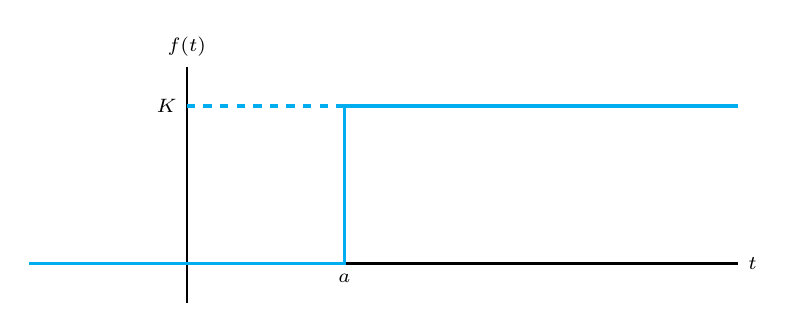
\begin{tikzpicture}
				\begin{scope}[thick,font=\scriptsize]
				% Axes:
				% Are simply drawn using line with the `->` option to make them arrows:
				% The main labels of the axes can be places using `node`s:
				\draw (-2,0) -- (7,0) node [right] {\(t\)};
				\draw  (0,-0.5) -- (0,2.5) node [above] {\(f(t)\)};
				
				% Axes labels:
				% Are drawn using small lines and labeled with `node`s. The placement can be set using options
				\iftrue% Single
				% If you only want a single label per axis side:
				\node [below] at (2,0) {\(a\)};
				\node [left] at (0,2) {\(K\)};
				
				\else% Multiple
				% If you want labels at every unit step:
				\foreach \n in {-4,...,-1,1,2,...,4}{%
					\draw (\n,-3pt) -- (\n,3pt)   node [above] {$\n$};
					\draw (-3pt,\n) -- (3pt,\n)   node [right] {$\n i$};
				}
				\fi
				\end{scope}
				
				\draw[cyan, very thick] (-2,0) -- (2,0) -- (2,2) -- (7,2);
				\draw[cyan, very thick, dashed] (0,2) -- (2,2);

				
				% Place the equation into the circle:
				\end{tikzpicture}
				\caption{A step function occuring at \(t=a\) when \(a>0\)}
			\end{figure}
			
			\begin{mitteks} [Shifted Unit Step Function] 
			\[f(t)=u(t-3)\]
			
			Ligningen betyr at \(f(t)\) har verdi 0 når \(t<3\) og 1 når \(t>3\). Den ser slik ut	
			\end{mitteks}
			
						\begin{figure}[!ht]
							\centering
							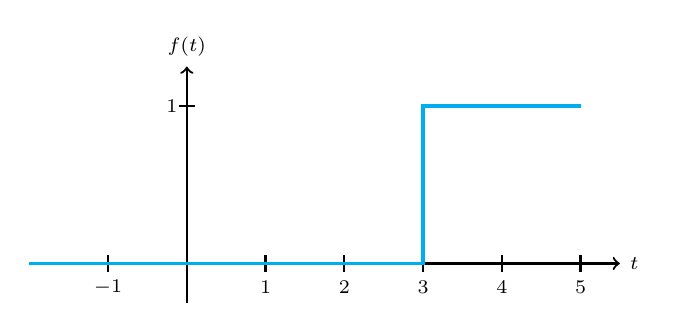
\begin{tikzpicture}
							\begin{scope}[thick,font=\scriptsize]
							% Axes:
							% Are simply drawn using line with the `->` option to make them arrows:
							% The main labels of the axes can be places using `node`s:
							\draw [->] (-1.5,0) -- (5.5,0) node [right] {\(t\)};
							\draw [->]  (0,-.5) -- (0,2.5) node [above] {\(f(t)\)};
							
							% Axes labels:
							% Are drawn using small lines and labeled with `node`s. The placement can be set using options
							\iffalse% Single
							% If you only want a single label per axis side:
							\node [below] at (2,0) {\(a\)};
							\node [left] at (0,2) {\(K\)};
							
							\else% Multiple
							% If you want labels at every unit step:
							\foreach \n in {-1,...,-1,1,2,...,5}{%
								\draw (\n,-3pt) -- (\n,3pt)   node at (\n,-0.3) {\(\n\)};
							}
							\draw (-3pt,2) -- (3pt,2) node [left] {1 \hspace{3pt}};
							\fi
							\end{scope}
							
							\draw[cyan, very thick] (-2,0) -- (3,0) -- (3,2) -- (5,2);
							
							
							
							% Place the equation into the circle:
							\end{tikzpicture}
							\caption{\(f(t)=u(t-3)\)}
						\end{figure}
						
		\newpage
		\subsection{Firkant puls}
		
		\begin{fmindef}
		En vanlig situasjon i en krets er å tilføre spenning til et gitt tidspunkt t=a og ta den vekk senere, t=b. Vi skriver en slik situasjon ved å bruke "step function" slik \[V(t)=K[u(t-a)-u(t-b)]\] Denne spenningen har styrke K, i perioden (b-a).	
		\end{fmindef}
		
		\begin{mitteks}
			Grafen til \(V(t)=0.9[u(t-1.2)-u(t-3.8)]\) er som følger. Perioden er \(3.8-1.2=2.6\)
		\end{mitteks}
		
			\begin{figure}[!ht]
				\centering
				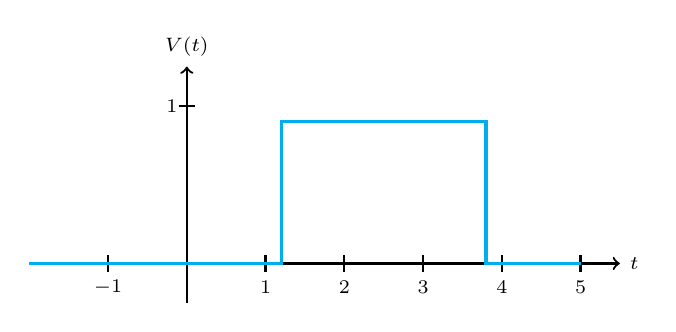
\begin{tikzpicture}
				\begin{scope}[thick,font=\scriptsize]
				% Axes:
				% Are simply drawn using line with the `->` option to make them arrows:
				% The main labels of the axes can be places using `node`s:
				\draw [->] (-1.5,0) -- (5.5,0) node [right] {\(t\)};
				\draw [->]  (0,-.5) -- (0,2.5) node [above] {\(V(t)\)};
				
				% Axes labels:
				% Are drawn using small lines and labeled with `node`s. The placement can be set using options
				\iffalse% Single
				% If you only want a single label per axis side:
	
				
				\else% Multiple
				% If you want labels at every unit step:
				\foreach \n in {-1,...,-1,1,2,...,5}{%
					\draw (\n,-3pt) -- (\n,3pt)   node at (\n,-0.3) {\(\n\)};
				}
				\draw (-3pt,2) -- (3pt,2) node [left] {1 \hspace{3pt}};
				\fi
				\end{scope}
				
				\draw[cyan, very thick] (-2,0) -- (1.2,0) -- (1.2,1.8) -- (3.8,1.8) -- (3.8,0) -- (5,0);
				
				
				
				% Place the equation into the circle:
				\end{tikzpicture}
				\caption{\(V(t)=0.9[u(t-1.2)-u(t-3.8)]\) }
			\end{figure}
			
	    \newpage
	    
	    \begin{mitteks}
	    	Tegn grafen til \[f(t)=3t^2\cdot[u(t)-u(t-2)]+12\cdot [u(t-2)-u(t-4)]+(4t-28)\cdot [u(t-4)-u(t-7)] \]
	    \end{mitteks}
	    
	    			\begin{figure}[!ht]
	    				\centering
	    				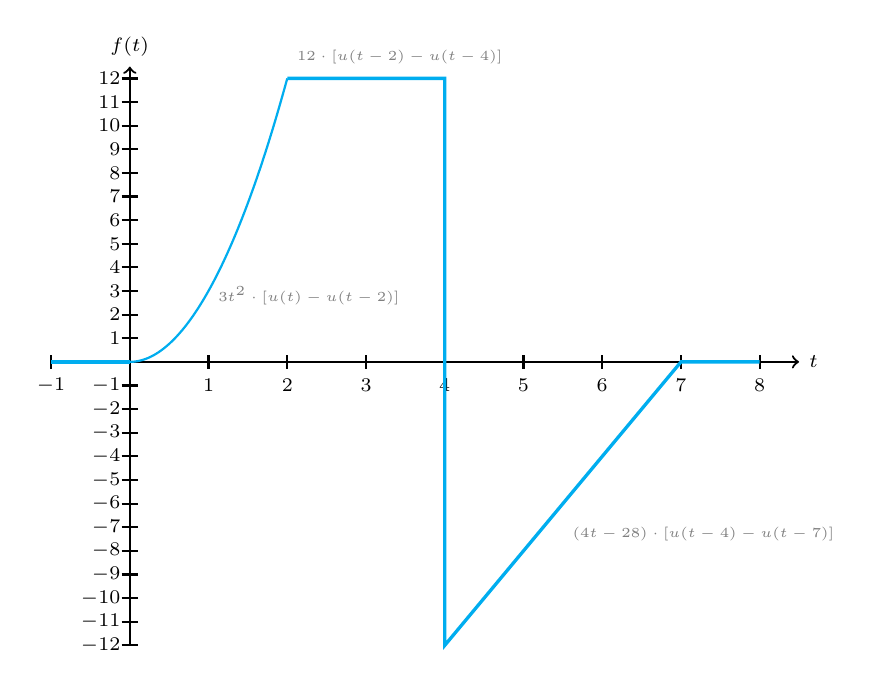
\begin{tikzpicture}[xscale=1,yscale=0.3]
	    				\begin{scope}[thick,font=\scriptsize]
	    				% Axes:
	    				% Are simply drawn using line with the `->` option to make them arrows:
	    				% The main labels of the axes can be places using `node`s:
	    				\draw [->] (-1,0) -- (8.5,0) node [right] {\(t\)};
	    				\draw [->]  (0,-12) -- (0,12.5) node [above] {\(f(t)\)};
	    				
	    				% Axes labels:
	    				% Are drawn using small lines and labeled with `node`s. The placement can be set using options
	    				\iffalse% Single
	    				% If you only want a single label per axis side:
	    				
	    				
	    				\else% Multiple
	    				% If you want labels at every unit step:
	    				\foreach \n in {-1,...,-1,1,2,...,8}{%
	    					\draw (\n,-0.3cm) -- (\n,0.3cm)   node at (\n,-1cm) {\(\n\)};
	    				}
	    				
	         			\foreach \n in {-12,...,-1,1,2,...,12}{%
	    					\draw (-3pt,\n) -- (3pt,\n) node [left] {\(\n\) \hspace{3pt}};
	    		    	}
	    				
	    				\fi
	    				\end{scope}
	    				
	    				\draw[cyan, very thick] (-1,0) -- (0,0);
	    				
	    				\draw[cyan, very thick] (2,12) -- (4,12) -- (4,-12) -- (7,0) -- (8,0);
	    				
	    			    \draw[cyan,thick] (0,0) parabola bend (0,0) (2,12);
	    			    	    			            
	    				\node [above right,gray] at (1,2) {\tiny \(3t^2\cdot[u(t)-u(t-2)]\)};	
	    				\node [above right,gray] at (2,12.2) {\tiny \(12\cdot [u(t-2)-u(t-4)]\)};
	    				\node [above right,gray] at (5.5,-8) {\tiny \((4t-28)\cdot [u(t-4)-u(t-7)]\)};
	    				\end{tikzpicture}
	    				\caption{Grafen til \(f(t)\)}
	    			\end{figure}
		\newpage
		
		\def\arraystretch{2.5}%
		\begin{table}[!ht]
			\centering
			\caption{Basisformler for Laplace-transformasjon}
			\label{my-label}
			\begin{tabular}{p{4cm} p{4cm} l}
				\hline
 				\textbf{Type} & \textbf{f(t)}          & \textbf{F(s)}                        \\ \hline
				impulse       & \(\delta(t)\)          & 1                                    \\ \hline
				step          & u(t)                   & \(\dfrac{1}{s}\)                     \\ \hline
				ramp          & t                      & \(\dfrac{1}{s^2}\)                   \\ \hline
				exponential   & \(e^{-at}\)                 & \(\dfrac{1}{s+a}\)                   \\ \hline
				sine          & \(sin \omega t\)       & \(\dfrac{\omega }{s^2+\omega^2}\)    \\ \hline
				cosine        & \(cos\omega t\)        & \(\dfrac{s}{s^2+\omega^2}\)          \\ \hline
				damped ramp   & \(te^{-at} \)          & \(\dfrac{1}{(s+a)^2}\)               \\ \hline
				damped sine   & \(e^{-at}sin\omega t\) & \(\dfrac{\omega}{(s+a)^2+\omega^2}\) \\ \hline
				damped cosine & \(e^{-at}cos\omega t\) & \(\dfrac{s+a}{(s+a)^2+\omega^2}\)      \\ \hline
			\end{tabular}
		\end{table}
	
	\def\arraystretch{1}%
	\newpage 

\begin{mindef}[Kjente resultater om laplacetransformer] \leavevmode
		\begin{enumerate}
		\item \(\mathscr{L}(1)=\dfrac{1}{s},s>0\)
		\item \(\mathscr{L}(t^n)=\dfrac{n!}{s^{n+1}},s>0\)
		\item \(\mathscr{L}(e^{at})=\dfrac{1}{s-a},s>a\)
		\item \(\mathscr{L}(t^ne^{at})=\dfrac{n!}{(s-a)^{n+1}},s>a\)
		\item \(\mathscr{L}(sin(\alpha t))=\dfrac{\alpha}{s^2+\alpha^2},s>0\)
		\item \(\mathscr{L}(cos(\alpha t))=\dfrac{s}{s^2+\alpha^2},s>0\)
		\item \(\mathscr{L}(e^{\beta t} sin(\alpha t))=\dfrac{\alpha}{(s-\beta)^2+\alpha^2},s>\beta\)
		\item \(\mathscr{L}(e^{\beta t }cos(\alpha t))=\dfrac{s-\beta}{(s-\beta)^2+\alpha^2},s>\beta\)
		\item \(\mathscr{L}(\delta (t))=1,\mathscr{L}(\delta (t-c))=e^{-cs}\)
		\item \(\mathscr{L}(f^\prime)=s\mathscr{L}-f(0)\)
		\item \(\mathscr{L}(f^{\prime \prime})=s^2\mathscr{L}(f)-sf(0)-f^\prime (0)\)
		\item \(\mathscr{L}(f(t-a)u(t-a))=e^{-as}F(s)=e^{-as}\mathscr{L}(f(t)), der\,\, u(t-a)= \begin{cases}
		0,\,\, t<a \\
		1,\,\, t\ge a 
		\end{cases}\) er Heaviside-funksjonen
		\item \(\mathscr{L}(af+bg)=a\mathscr{L}(f)+b\mathscr{L}(g)\)
    	\end{enumerate}
\end{mindef}

\newpage

\section{Funksjoner av flere variabler}

\subsection{Gradient og retningsderivert}

\begin{fmindef}[Gradient]
	La \(f(x,y)\) være en deriverbar funksjon, og \(\vec{i} \),  \(\vec{j} \) standardbasisen for \(\mathbb{R}^2 \). 
	\[\nabla f=\frac{\partial f}{\partial x}\vec{i}+\frac{\partial f}{\partial y}\vec{j}=\left(\frac{\partial f}{\partial x}+\frac{\partial f}{\partial y} \right) \]
	
	\textit{gradienten} til funksjonen. Om vi evaluerer i et punkt \((a,b) \), får vi gradienten i punktet:
	
	\[\nabla f\big|_{(a,b)} =\frac{\partial f}{\partial x}\Big|_{(a,b)} \vec{i}+\frac{\partial f}{\partial y}\Big|_{(a,b)} \vec{j} \]
\end{fmindef}

\begin{fteo}[Geomatrisk tolkning av gradienten]
	
	La \(f(x,y)\) være en funksjon slik at de partielt deriverte er kontinuerlige.
	Da gjelder disse egenskapene for gradienten i et punkt \((a,b)\):
	\begin{itemize}
		\item Gradienten \(\nabla f\big|_{(a,b)} \) er en normalvektor til nivåkurven for \(f\) gjennom punktet \((a,b)\).
		\item Gradienten \(\nabla f\big|_{(a,b)} \) peker i den bratteste retningen på grafen \(z=f(x,y)\).
		\item Lengden av gradienten \(\left| \nabla f\big|_{(a,b)} \right| \) er stigningstallet til grafen i den bratteste retningen.
	\end{itemize}
	
\end{fteo}

\begin{fmindef}
	La \(f(x,y)\) være en funksjon i to variabler som er deriverbar i punktet \((a,b)\), og la \(\vec{u}=[u_1,u_2] \) være en retning gitt ved en enhetsvektor (altså er \(u_1^2+u_2^2=1\)). Den \textit{retningsderiverte} til \(f\) i punktet \((a,b)\) og i retning \(u\) defineres som skalarproduktet \[D_{\vec{u}}f(a,b)=\vec{u}\cdot \nabla \big|_{(a,b)}. \]
	Dette angir altså hvor raskt funksjonsverdien endrer seg i retning bestemt av \(\vec{u} \).
\end{fmindef}

\newpage

\subsubsection{Ekstremalverdier for funksjoner i flere variabler}

\begin{fmindef}[Tangentplan]
	La \(f(x,y) \) være en funksjon som er deriverbar i \( (a,b)\). Da er ligningen for tangentplanet i punktet
	\[z=f(a,b)+f_x(a,b)\cdot (x-a)+f_y(a,b)\cdot (y-b) \]
\end{fmindef}

\begin{fmindef}
	Determinanten til Hesse-matrisen kalles \textit{diskriminanten} og er gitt ved 
	\[\Delta =\det{H}=\left| \begin{array}{rr} 
	f_{xx} & f_{yx} \\
	f_{xy} & f_{yy}
	\end{array} \right|=f_{xx}(a,\,b)\cdot f_{yy}(a,\,b)-\left( f_{xy}(a,\,b)\right)^2  \]
\end{fmindef}

\begin{fteo}[Andrederiverttesten for funksjoner i to variabler]
	La \(f(x,y)\) være en funksjon slik at de partielt deriverte av andre orden er kontinuerlige. Et stasjonært punkt \((a,\,b) \) til \(f\) kan klassifiseres ut fra Hesse-matrisen etter følgende kriterier:
	\begin{enumerate}
		\item Når \(\Delta >0 \) og \(f_{xx}(a,\,b) <0\),  er \((a,\,b) \) et lokalt maksimum.
		\item Når \(\Delta>0 \) og \(f_{xx}(a,\,b)>0 \), er \((a,\,b) \) et lokalt minimum.
		\item Når \(\Delta < 0  \), er \((a,\,b)\) et sadelpunkt.
		\item Når \(\Delta =0 \), gir testen ingen informasjon; alle muligheter er fortsatt åpne.
	\end{enumerate}
\end{fteo}
	
\end{document}